\documentclass[10pt]{beamer}
\usepackage[utf8]{inputenc}
\usepackage[french]{babel}
\usepackage[T1]{fontenc}
\usepackage{beamerthemesplit}
\usepackage{graphics,epsfig, subfigure}
\usepackage{url}
\usepackage{siunitx}
\usepackage{fourier}
\usepackage{tikz}
\usepackage{numprint}

\DeclareSIUnit\year{yr}

\definecolor{jd_blue0}{rgb}{0.51,0.34,1.00}
\definecolor{jdbishop}{rgb}{0.27,0.14,0.29}
\definecolor{jddarkbl}{rgb}{0.18,0.14,0.29}
\definecolor{jd_brown}{rgb}{0.29,0.14,0.14}
\definecolor{jd_green}{HTML}{096F35}
\definecolor{jdorange}{rgb}{1.00,0.55,0.00}
\definecolor{jdredred}{rgb}{0.50,0.00,0.00}
\definecolor{SchoolColor}{rgb}{0.145,0.666,1}
\definecolor{pheniics}{HTML}{1a899c}
\definecolor{pheniics_purple}{HTML}{64003d}
\definecolor{chaptercolor}{gray}{0.8}
\mode<presentation>
{  \usetheme{PaloAlto}

  \setbeamercolor{palette primary}{bg=pheniics,fg=white}
  \setbeamercolor{palette secondary}{bg=pheniics_purple,fg=white}
  \setbeamercolor{palette tertiary}{bg=pheniics_purple,fg=white}
  \setbeamercolor{palette quaternary}{bg=pheniics_purple,fg=white}
  \setbeamercolor{palette sidebar primary}{fg=white}
  \setbeamercolor{palette sidebar secondary}{fg=white}
  \setbeamercolor{palette sidebar tertiary}{fg=pheniics_purple}
  \setbeamercolor{palette sidebar quaternary}{fg=pheniics_purple}
  \setbeamercolor{structure}{fg=pheniics} % itemize, enumerate, etc
  \setbeamercolor{section in toc}{fg=black}

  \useinnertheme{circles}
  \usefonttheme[onlymath]{serif}
  \setbeamercovered{transparent}
  \setbeamertemplate{blocks}[rounded][shadow=true]
  \setbeamertemplate{navigation symbols}{}
  \addtobeamertemplate{footline}{
    \usebeamercolor[fg]{author in sidebar}
    \vskip-1cm\hskip15pt
    \insertframenumber\,/\,\inserttotalframenumber\kern1em\vskip2pt%
  }
}
\setbeamercovered{invisible}
%\setbeamertemplate{background}{\includegraphics[width=1\textwidth]{natfak_baggrund.pdf}}

\graphicspath{{../Chapitre_1/pictures/}{../Chapitre_2/pictures/}{../Chapitre_3/pictures/}{../Chapitre_4/pictures/}{../Chapitre_5/pictures/}{../Front-back_covers/images/}{pictures/}}
 
\logo{
\includegraphics[width=1.5cm]{logo_CEA.png}}
\title[Le projet WA105]{Le projet WA105 : un prototype de Chambre à Projection Temporelle à Argon Liquide Diphasique utilisant des détecteurs LEMs}
\author{Présenté par \\ \textbf{Philippe Cotte} \\ \vspace{0.3cm} Sous la direction de \\ \textbf{E. Mazzucato}\vspace{-0.2cm}}
\institute{CEA Paris-Saclay \\ Université Paris-Saclay\vspace{-0.2cm}}
\date{\vspace{-0.2cm}17 Septembre 2019}

\def\TOO{\SI{4}{\tonne}}
\def\SSS{\SI{300}{\tonne}}
\def\threeL{\SI{3}{\liter}}
\def\dune{DU$\nu$E}
\def\checkmark{\tikz\fill[scale=0.4](0,.35) -- (.25,0) -- (1,.7) -- (.25,.15) -- cycle;}

\newenvironment{specialframe}
{
    \begingroup
    \advance\textwidth2cm % see beamerthemeGoettingen.sty for the number
    \hsize\textwidth
    \columnwidth\textwidth
    \begin{frame}[plain]
}
{
    \end{frame}
    \endgroup
}

\tracksfalse

\begin{document}

    {
        \usebackgroundtemplate{
\includegraphics[width=\paperwidth]{./pictures/1.pdf}}
        \begin{specialframe}
            \vspace{2cm}\hspace*{-1.8cm}\parbox[t]{\textwidth}{\titlepage}
        \end{specialframe}
    }
    \begin{specialframe}{Table des matières}
        \begin{textblock*}{\textwidth}(1cm,0.35\textheight)
            \tableofcontents[hideallsubsections]
        \end{textblock*}
    \end{specialframe}

  \setcounter{framenumber}{0}
    {
    	\usebackgroundtemplate{
\includegraphics[width=\paperwidth]{./pictures/1.pdf}}
        \begin{specialframe}
            \vspace{2cm}\hspace*{-1.8cm}\parbox[t]{\textwidth}{
                \begin{center}
                    \begin{huge}
                            \textcolor{pheniics_purple}{\textbf{Contexte physique et expérimental}}
                    \end{huge}
                    \vspace{1cm}
                    \begin{enumerate}
                        \item Le CERN, les neutrinos et l'expérience DU$\nu$E 
                        \item TPCs à argon liquide Simple phase et Double phase
                        \item Les détecteurs gazeux MPGD (LEMs) de WA105
                    \end{enumerate}
                \end{center}
            }
        \end{specialframe}
    }

  \section[Contexte]{Contexte physique et expérimental}
    
    \begin{frame}{La plateforme neutrino du CERN}{ProtoDU$\nu$E--SP et WA105/ProtoDU$\nu$E--DP}
        \begin{columns}
            \begin{column}{0.5\textwidth}
                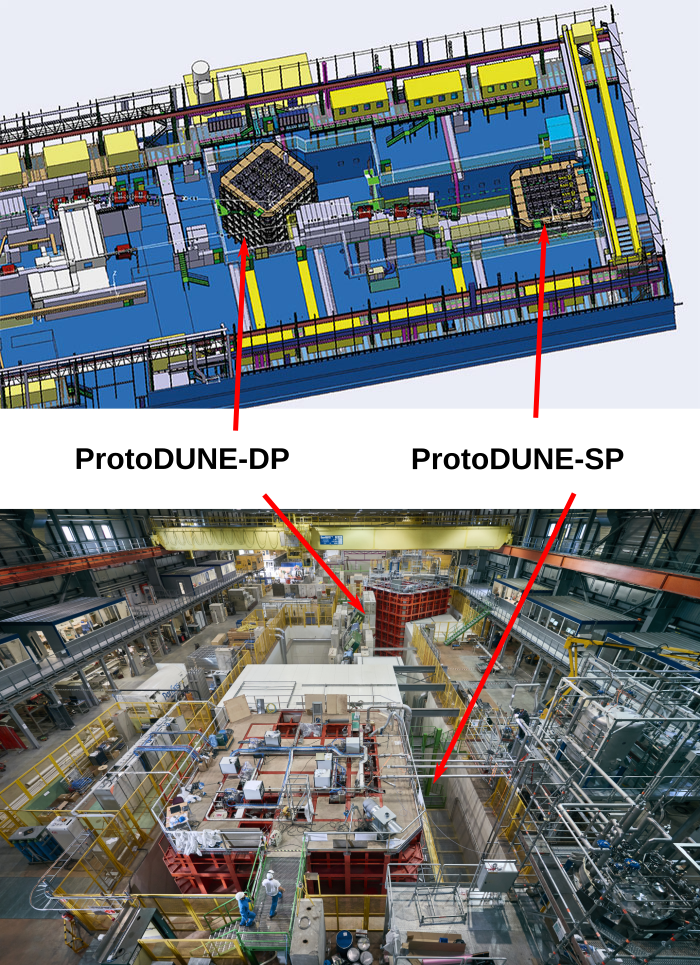
\includegraphics[height=0.9\textheight]{./pictures/neutrino_platform.png}
            \end{column}
            \begin{column}{0.5\textwidth}
                \begin{scriptsize}
                    Stratégie Européenne de physique des particules de 2013 : implication du CERN dans la recherche mondiale en physique des neutrinos : \\ $\Rightarrow$ Extension du hall de test en faisceau du site de Prévessin.\vspace{0.4cm}
                    \begin{itemize}
                        \item Prototypage de \textbf{Chambres à Projection Temporelle à Argon Liquide} : ProtoDU$\nu$-SP et \textcolor{red}{WA105/ProtoDU$\nu$E--DP}
                        \item Technologie choisie pour la future expérience d'oscillation des neutrinos DU$\nu$E
                        \item Tests en faisceaux et/ou en cosmiques
                    \end{itemize}
                \end{scriptsize}
            \end{column}
        \end{columns}
    \end{frame}
        
    \begin{frame}{Oscillations des neutrinos : les grandes inconnues}{Ordre des masses et violation de CP}
        \begin{columns}
            \begin{column}{0.5\textwidth}
                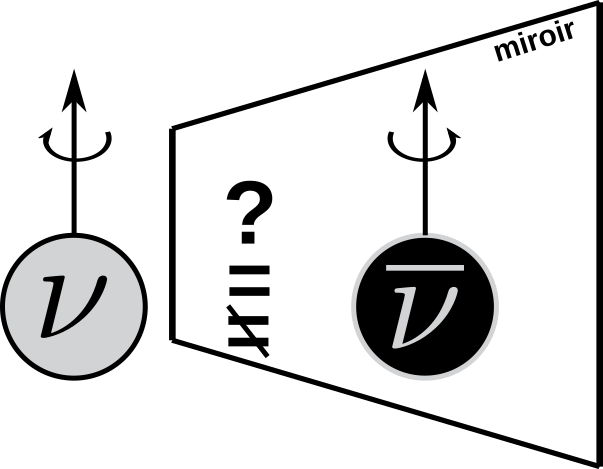
\includegraphics[width=0.8\textwidth]{./pictures/CP_schema.png}\\
                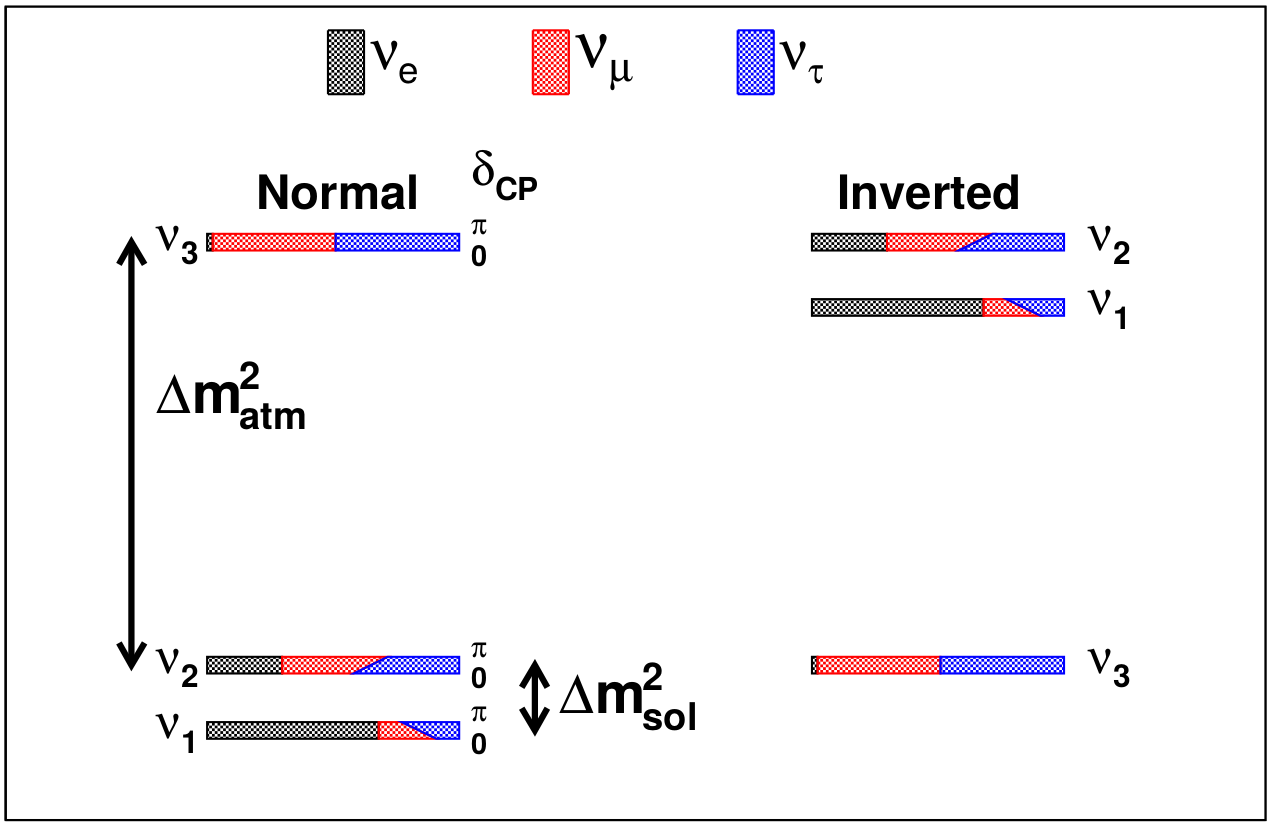
\includegraphics[width=\textwidth]{mass_hierarchy.png}
            \end{column}
            \begin{column}{0.5\textwidth}
                \begin{scriptsize}
                    \begin{itemize}
                        \item La symétrie CP est-elle violée dans le secteur leptonique?  \\ $\Rightarrow$ Pourrait expliquer l'asymétrie matière-antimatière de l'univers
                        \item Quel est l'ordre des masses des neutrinos?  \\ $\Rightarrow$ Contrainte sur certaines théories au delà du modèle standard 
                    \end{itemize}
                    \vspace{0.4cm}
                    \textbf{Connaissances actuelles :}
                \end{scriptsize}
                \begin{itemize}
                    \item \begin{scriptsize}$\delta_{CP} \ne 0$ ou $\pi$ à $2\sigma$ (i.e CP semble violée)\end{scriptsize} \\  \tiny{T2K, Physical Review Letters 121.17 (oct. 2018)}
                    \item \begin{scriptsize}3$\sigma$ en faveur de l'ordre des masses normal\end{scriptsize} \\ \tiny{NO$\nu$A, Physics Letters B 782 (juil. 2018), p. 633–640}
                \end{itemize}
            \end{column}
        \end{columns}
    \end{frame}

    \begin{frame}{DU$\nu$E : Deep Underground Neutrino Experiment}{Une expérience d'oscillation de neutrinos d'accélérateur à longue ligne de base}
        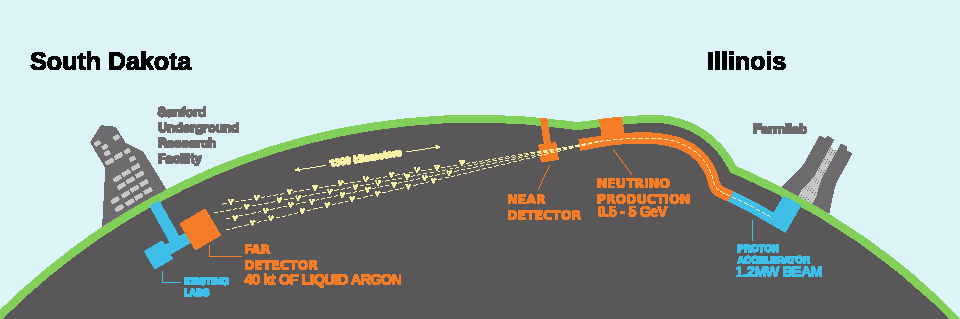
\includegraphics[width=\textwidth]{./pictures/dune.pdf}\\
        \begin{scriptsize}
        \vspace{0.4cm}
        \begin{columns}
            \begin{column}{0.75\textwidth}
                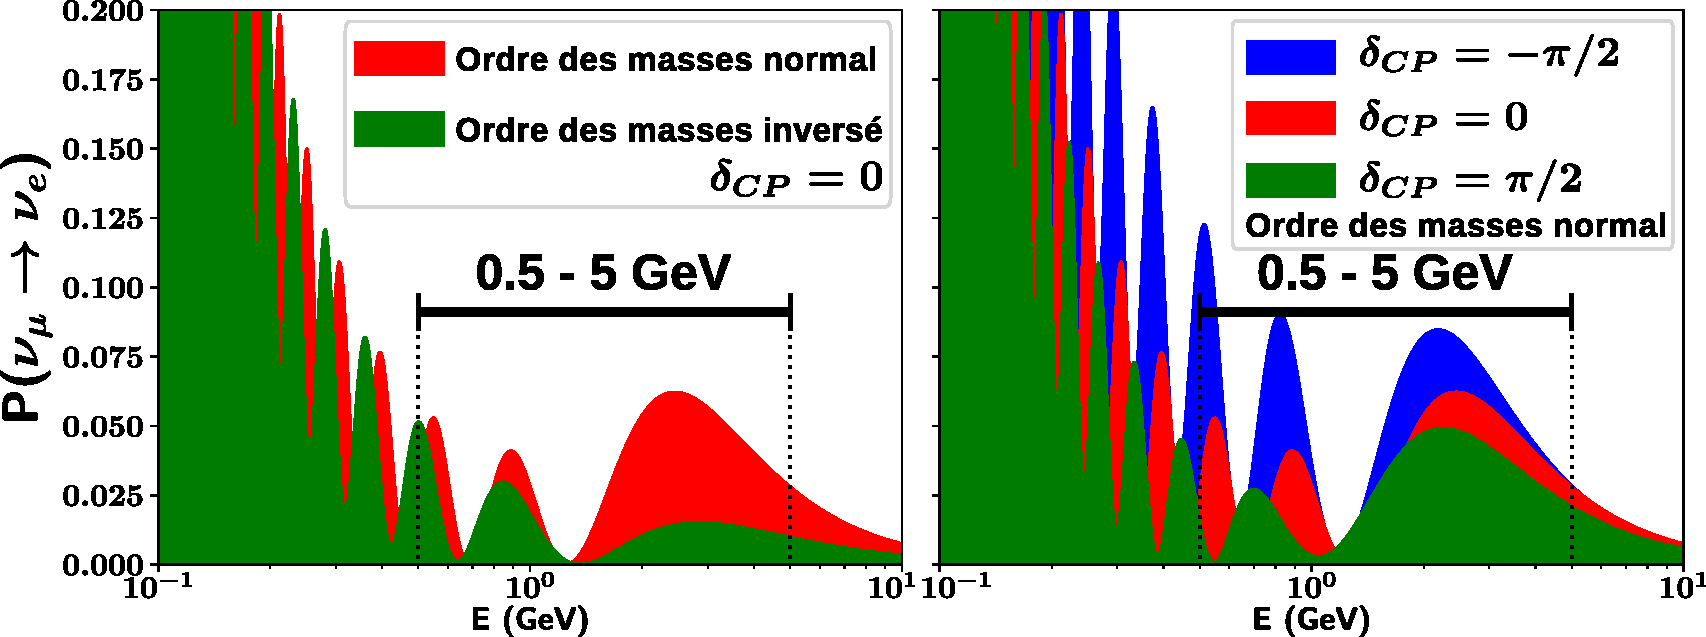
\includegraphics[width=\textwidth]{numu-nue-vs-E-MH-CP.pdf}
            \end{column}
            \hspace{-0.5cm}
            \begin{column}{0.35\textwidth}
                 \begin{itemize}
                     \item Les $\nu_{\mu}$ initiaux ont une probabilité $P(\nu_{\mu}\to\nu_e)$ d'être des $\nu_e$ à l'arrivée
                     \item \textcolor{red}{$P(\nu_{\mu}\to\nu_e)$} vs $E$ dépend de \textcolor{red}{$\delta_{CP}$} et de l'\textcolor{red}{ordre des masses}
                     \item 50\,\% $\nu_{\mu}$ / 50\,\% $\overline{\nu}_{\mu}$ \\ $>$ 15 ans de prise de données à partir de fin 2026
                 \end{itemize}
            \end{column}
        \end{columns}
        \end{scriptsize}
    \end{frame}
    
    \subsection{DU$\nu$E}
    
    \begin{frame}{DU$\nu$E : Deep Underground Neutrino Experiment}{Sensibilités}
        \begin{scriptsize}
            \begin{columns}
                \begin{column}{0.45\textwidth}
                    \centering
%                    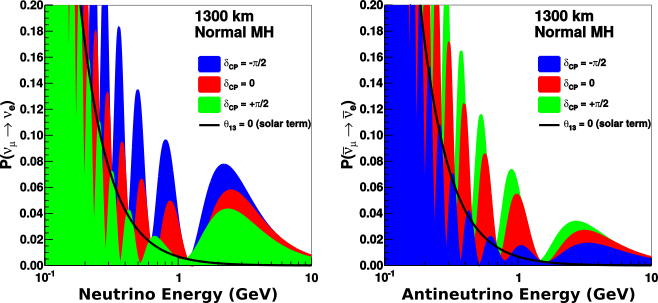
\includegraphics[width=\textwidth]{oscillation_CP.png} \\ \vspace{0.2cm}
                    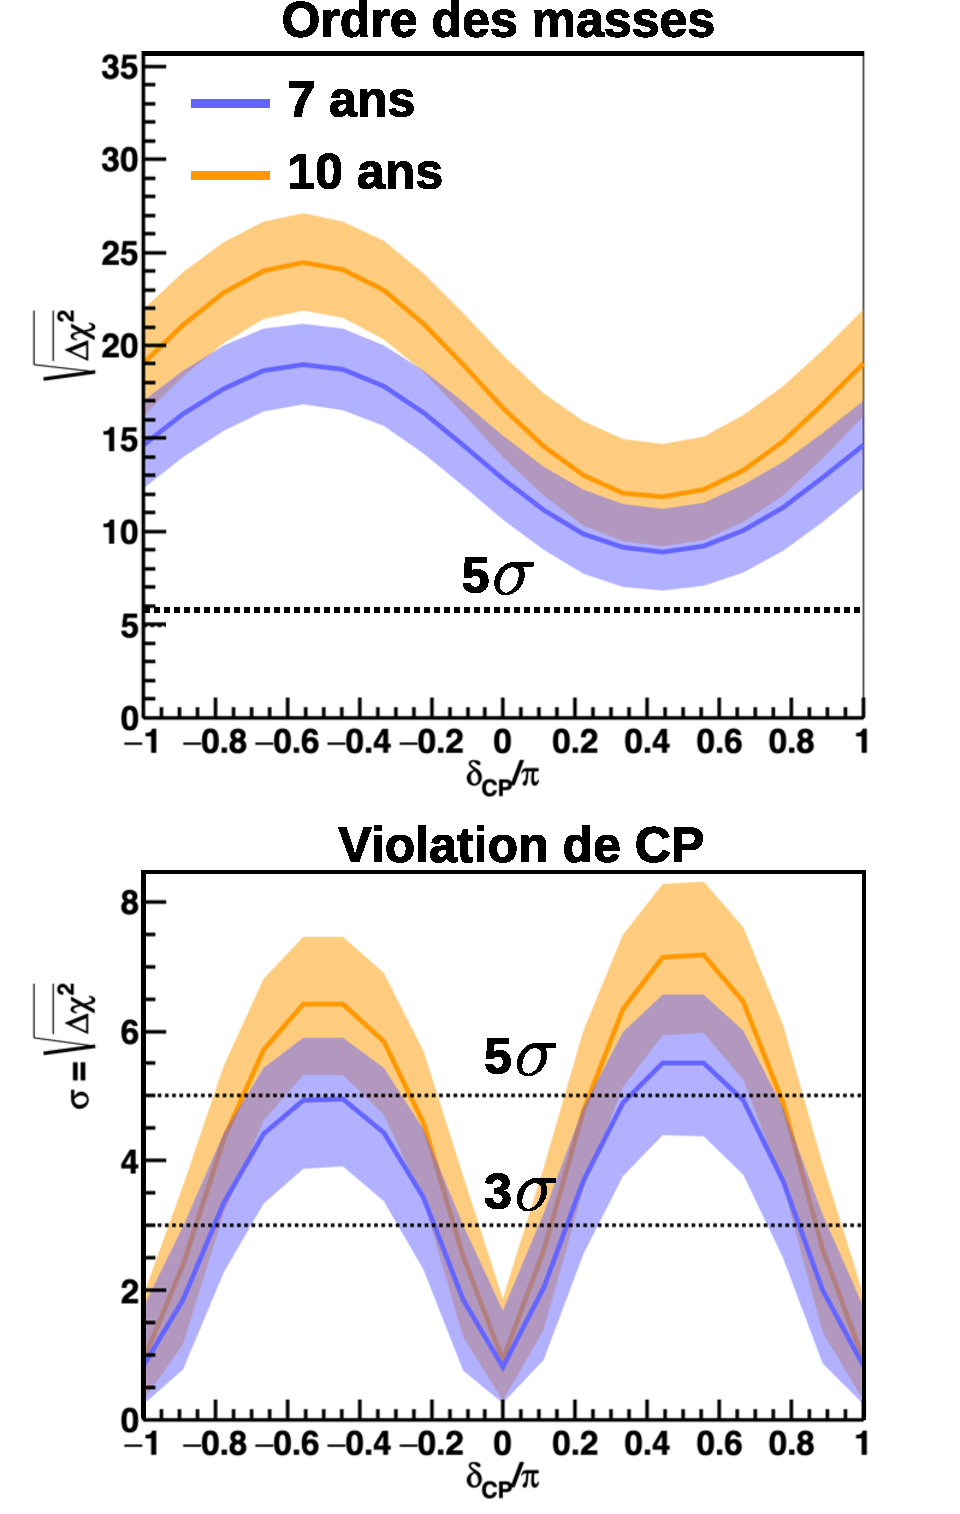
\includegraphics[width=1\textwidth]{sensitivities.pdf}
                \end{column}\hfill
                \begin{column}{0.55\textwidth}
                        \begin{tabular}{|l|l|}
                        \hline
                        \multicolumn{2}{|c|}{\textbf{Ordre des masses}} \\ \hline
                        & \\
                        \textbf{\begin{tabular}[c]{@{}l@{}}1 an
                        %\\ \SI{24}{\kilo\tonne\mega\watt\year}
                        \end{tabular}} & \begin{tabular}[c]{@{}l@{}}$5\sigma$\\  si $\delta_{CP}= -\frac{\pi}{2}$\end{tabular} \\
                        & \\
                        \textbf{\begin{tabular}[c]{@{}l@{}}2 ans
%                        \\ \SI{60}{\kilo\tonne\mega\watt\year}
                        \end{tabular}} & \begin{tabular}[c]{@{}l@{}}$5\sigma$\\ $\forall \delta_{CP}$\end{tabular} \\ \hline
                        \multicolumn{2}{|c|}{\textbf{Violation de CP}} \\ \hline
                        & \\
                        \textbf{\begin{tabular}[c]{@{}l@{}}7 ans\\ \SI{300}{\kilo\tonne\mega\watt\year}\end{tabular}} & \begin{tabular}[c]{@{}l@{}}$5\sigma$\\  si $\delta_{CP}=-\frac{\pi}{2}$\end{tabular} \\
                        & \\
                        \textbf{\begin{tabular}[c]{@{}l@{}}10 ans
%                        \\ \SI{528}{\kilo\tonne\mega\watt\year}
                        \end{tabular}} & \begin{tabular}[c]{@{}l@{}}$5\sigma$ pour 50\,\% \\ des valeurs de $\delta_{CP}$\end{tabular} \\ \hline
                        \multicolumn{2}{|c|}{\textbf{résolution sur} $\mathbf{\boldsymbol{\delta}_{CP}}$} \\ \hline
                        & \\
                        \textbf{\begin{tabular}[c]{@{}l@{}}8 ans
%                        \\ \SI{336}{\kilo\tonne\mega\watt\year}
                        \end{tabular}} & \begin{tabular}[c]{@{}l@{}}$10^{\circ}$ \\ si $\delta_{CP}=0$ ou $\pi$\end{tabular} \\
                        & \\
                        \textbf{\begin{tabular}[c]{@{}l@{}}12 ans
%                        \\ \SI{720}{\kilo\tonne\mega\watt\year}
                        \end{tabular}} & \begin{tabular}[c]{@{}l@{}}$20^{\circ}$ \\ si $\delta_{CP}=-\frac{\pi}{2}$ ou $\pi$\end{tabular} \\ \hline
                        \end{tabular}\\
                        \textbf{15 ans : \SI{1000}{\kilo\tonne\mega\watt\year}}\\
                        \vspace{0.2cm}
                        \textit{TDR de DU$\nu$E 2019}
                \end{column}
            \end{columns}
        \end{scriptsize}
    \end{frame}
    
    \begin{frame}{Prérequis du système de détection}
        \begin{scriptsize}
            \begin{columns}
                \begin{column}{0.5\textwidth}
                    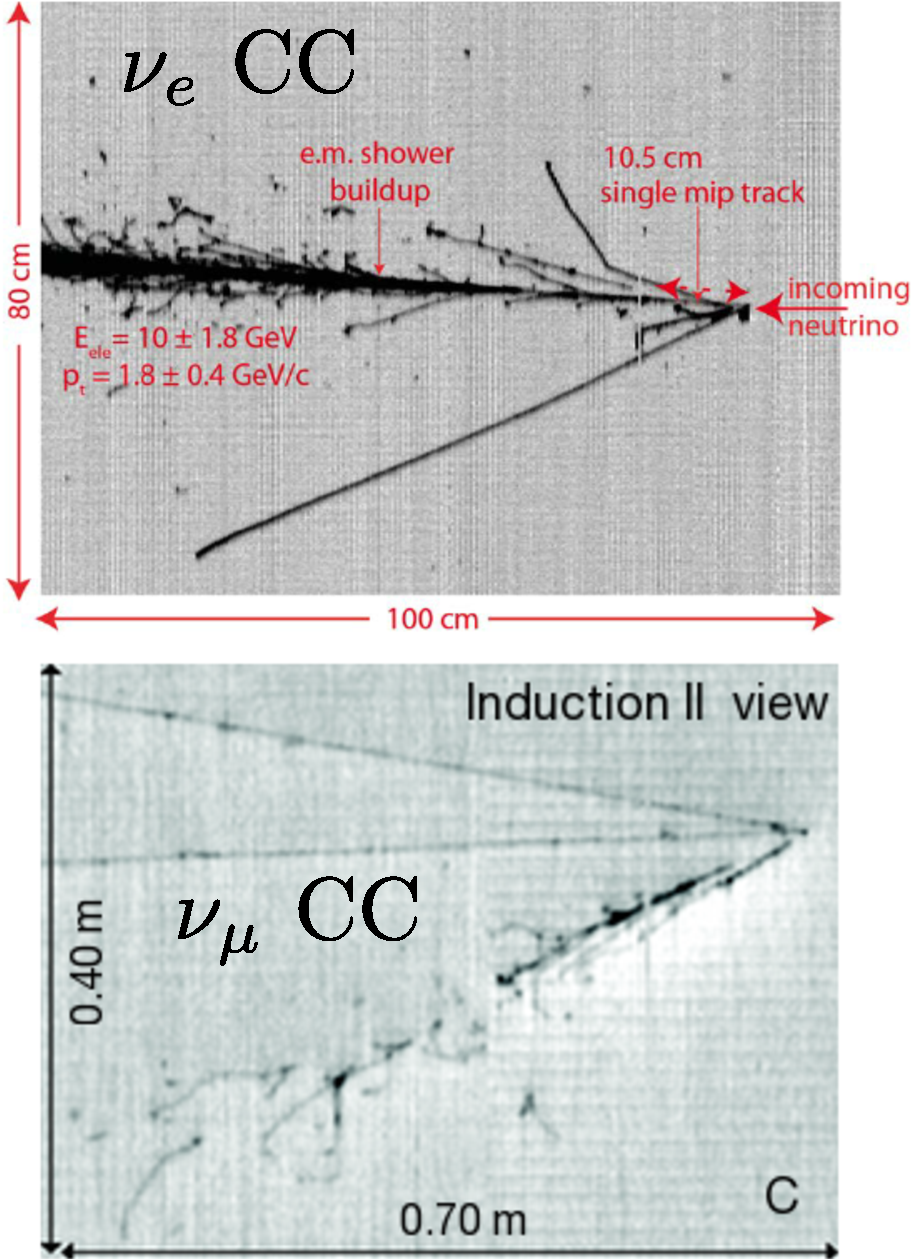
\includegraphics[width=\textwidth]{nu_events.pdf}\\\textit{Événements dans ICARUS T600 (2011)}
                \end{column}
                 \begin{column}{0.5\textwidth}
                    \begin{itemize}
                        \item Détection de neutrinos
                        \item Différencier $\nu_e$ et $\nu_{\mu}$ : \\ - $\neq dE/dx$ \\ - Gap en début de gerbe $\mathcal{O}(\si{\centi\meter})$
                        \item Neutrinos de supernovæ : \\ - très rare \\ - \SI{2}{\tera\byte\per\second} de données
                        \item Désintégration du proton $p\to \overline{\nu} + K^+$: \\ - trace de kaon $\mathcal{O}(\si{\centi\meter})$ \\ - Besoin d'un $t_0$ pour veto les bruits de fond
                    \end{itemize}
                    \begin{itemize}
                        \item[$\Rightarrow$] Multi-kilotonne
                        \item[$\Rightarrow$] Calorimètre
                        \item[$\Rightarrow$] Trajectographe 3D $\mathcal{O}(\si{\milli\meter})$
                        \item[$\Rightarrow$] PID
                        \item[$\Rightarrow$] Opération continue sur plusieurs années
                    \end{itemize}
                \end{column}
            \end{columns}
        \end{scriptsize}
    \end{frame}
                    
    \begin{frame}{L'argon liquide comme milieu de détection}
        \begin{scriptsize}
           	\begin{columns}
           		\begin{column}{0.6\textwidth}
           			\centering
           			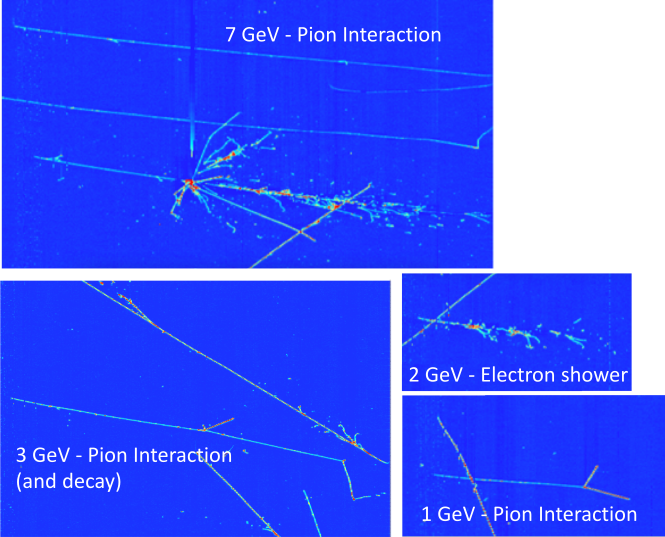
\includegraphics[width=\textwidth]{./pictures/SP_evt.png}\\
           			\flushleft
           			\begin{footnotesize}\textit{Événements dans ProtoDU$\nu$E--SP (08/2018)}\\
           			\textcolor{red}{Bruit $<$ \numprint{1000} $e^{-}$}\end{footnotesize}
           		\end{column}
           		\begin{column}{0.4\textwidth}
           			\begin{footnotesize}
           				\textbf{Pourquoi l'argon liquide?}
           			\end{footnotesize}
           			\begin{itemize}
           				\item Dense (\SI{1.4}{\gram\per\centi\meter^3})
           				\item Peu cher et abondant
           				\item Gaz noble $\rightarrow$ ne piège pas les électrons \textcolor{red}{(\danger impuretés!)}
           				\item Très bon trajectographe et calorimètre entièrement homogène
           				\item Scintille au moment de l'ionisation $\rightarrow$ déclencheur et/ou $t_0$ \\ + transparent pour les photons  d'ionisation
         				\item MIP $\rightarrow\sim\SI{60000}{e^-\per\centi\meter}$
           			\end{itemize}
           			\begin{footnotesize}
       	    			\textbf{$\Rightarrow$ Chambre à bulle électronique}
       	    		\end{footnotesize}
           		\end{column}
           	\end{columns}
        \end{scriptsize}
    \end{frame}

    \begin{frame}{Les 4 modules du détecteur lointain}{Deux SP, 1 DP, 1 à déterminer}
        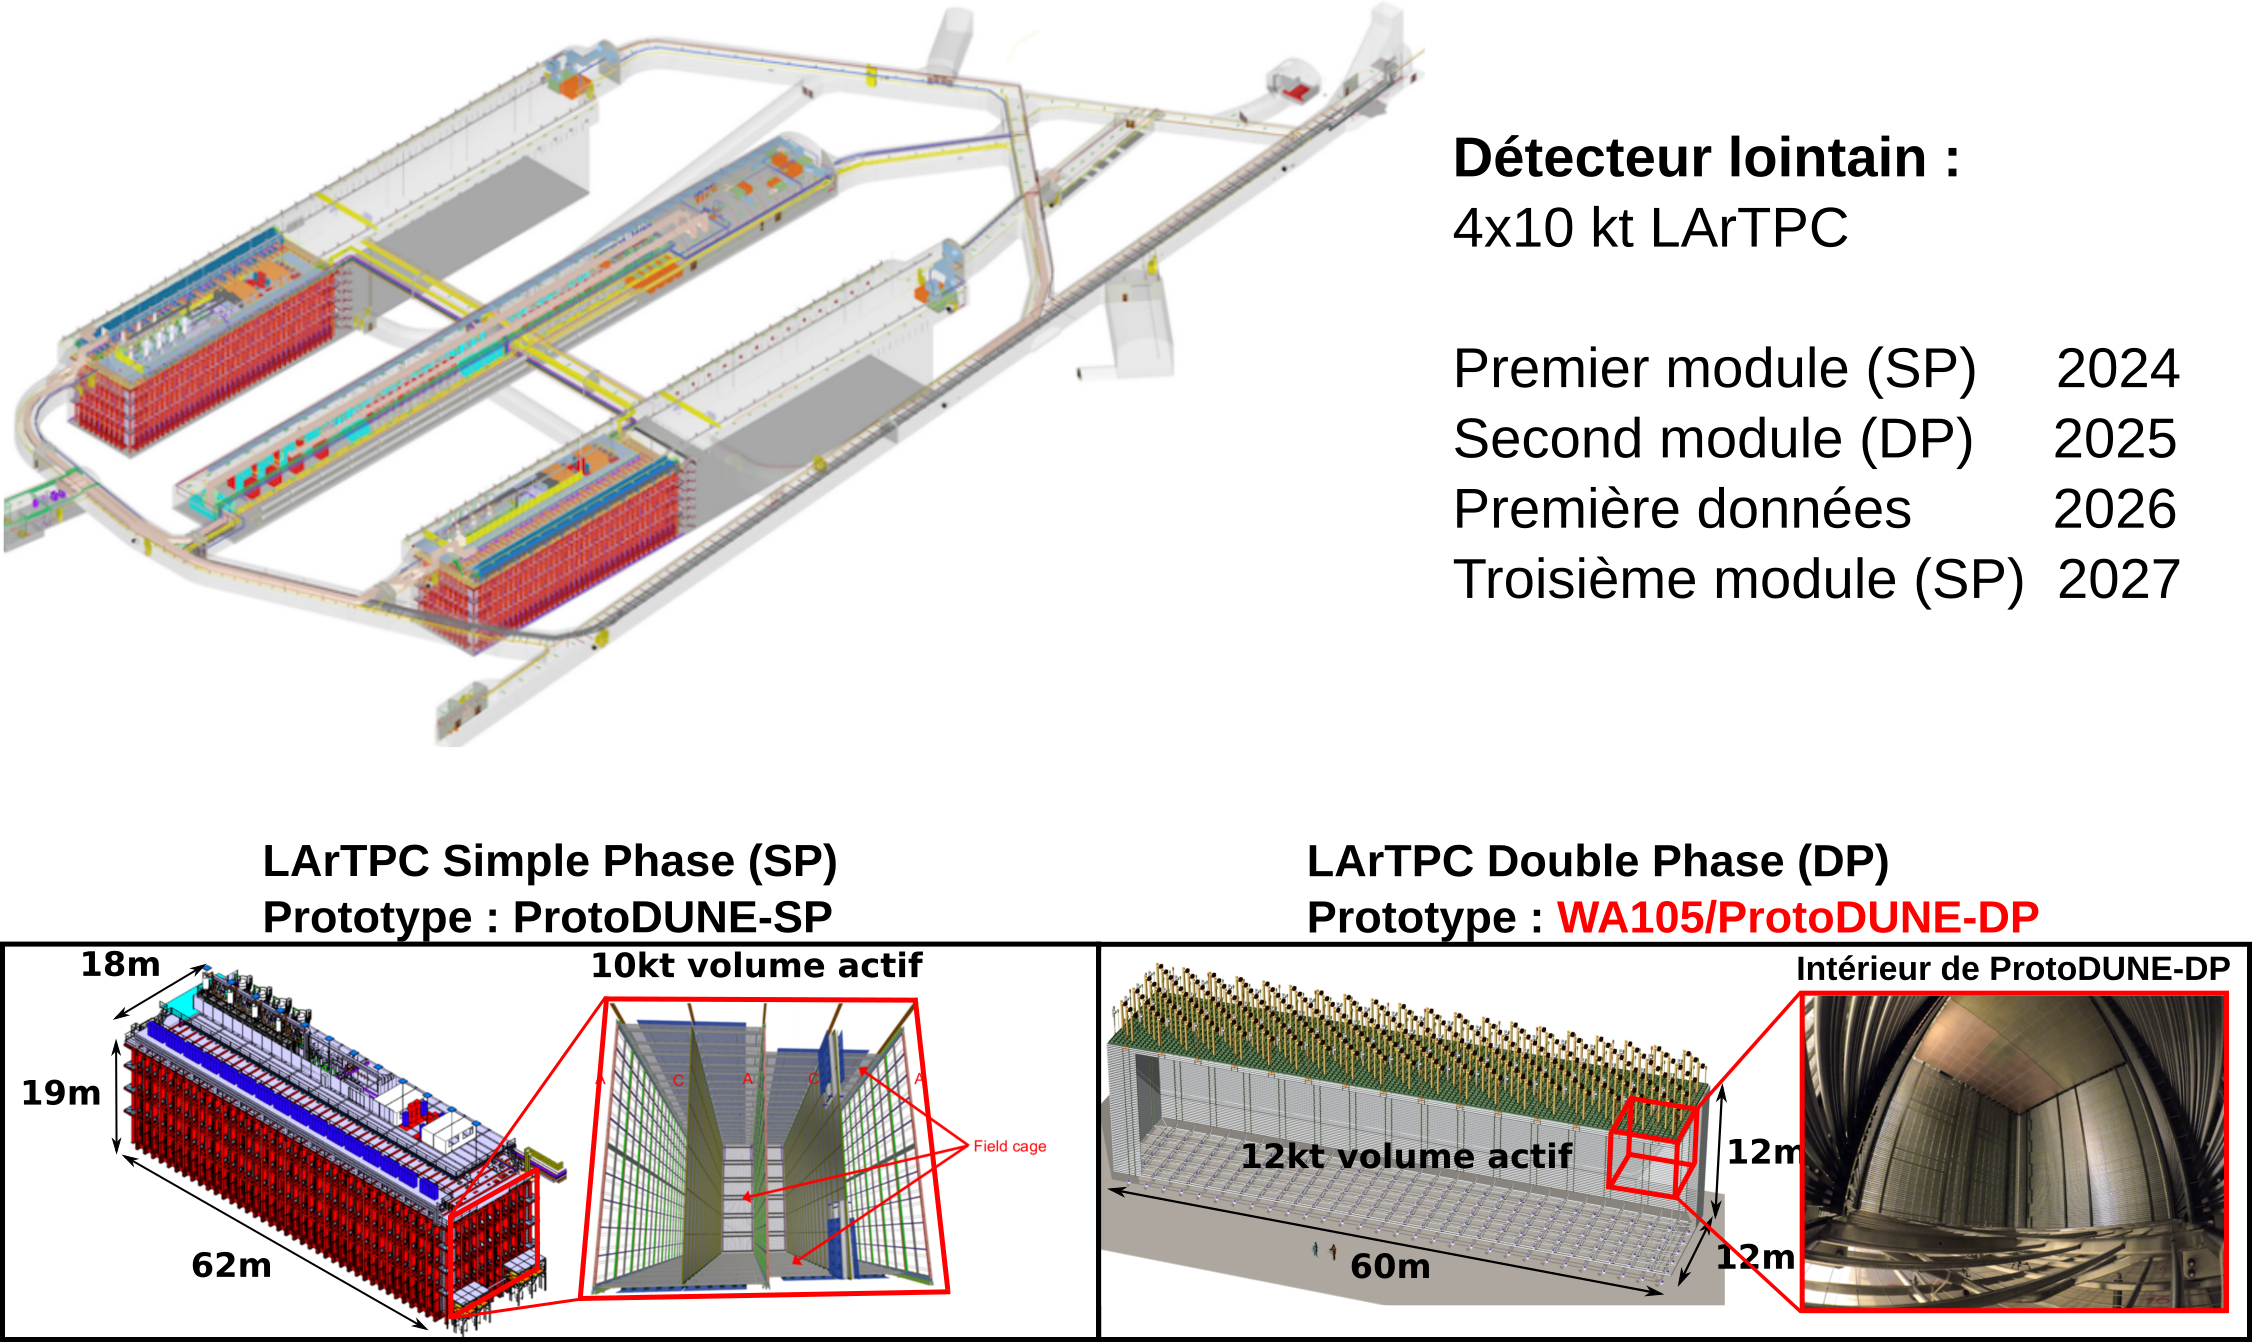
\includegraphics[width=\textwidth]{FD_full.pdf}
    \end{frame}
                
    \begin{frame}{La technologie LArTPC}{Chambres à Projection Temporelle à Argon Liquide}
       	\begin{scriptsize}
       			\centering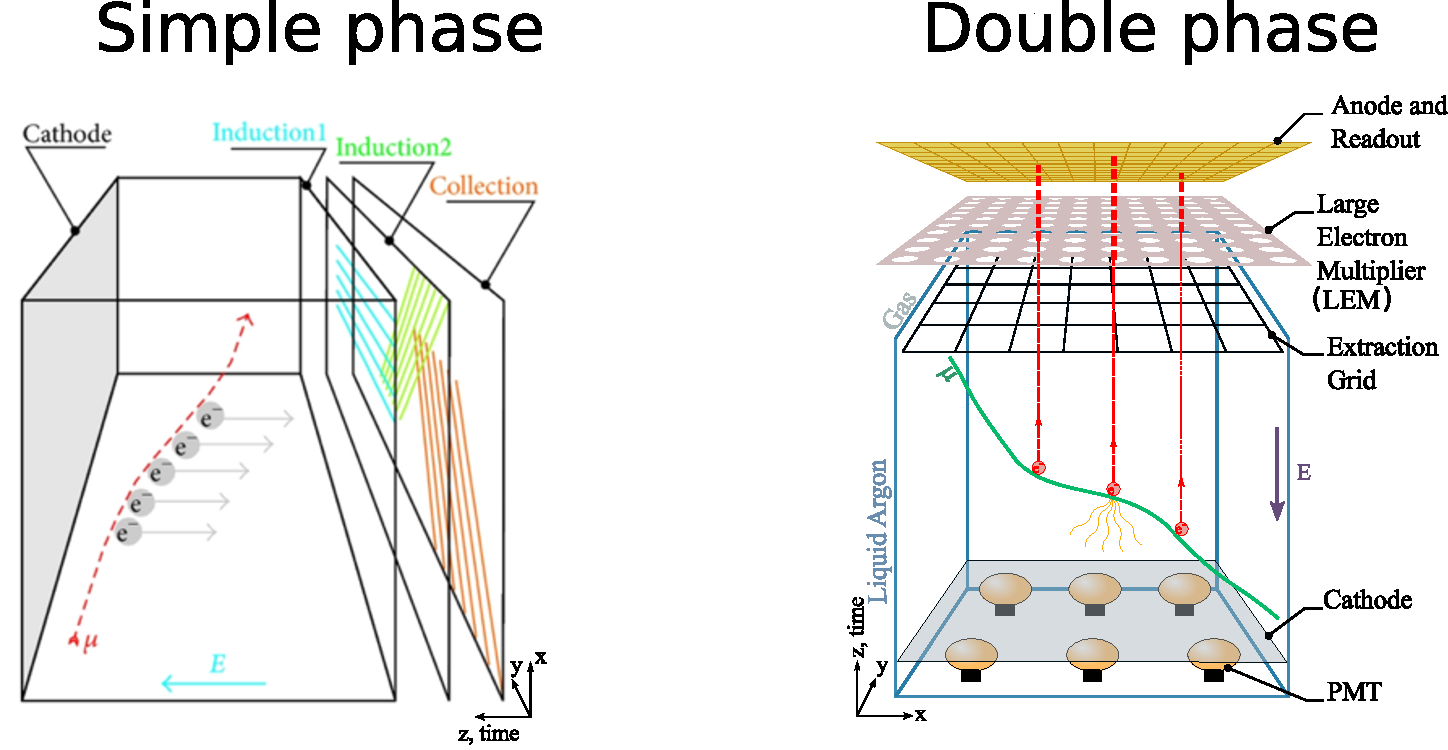
\includegraphics[width=0.95\textwidth]{./pictures/tpcs.pdf}\\
       			\begin{columns}
       				\begin{column}{0.5\textwidth}
       					\begin{itemize}
           					\item Tout se passe dans l'argon liquide
       						\item Reconstruction 3D des événements (précision millimétrique)
       						\item Mesure directe de l'énergie (précision $\sim\SI{100}{\kilo\electronvolt}$)
%       						\item Les premiers événements de protoDU$\nu$E-SP ont été vus l'an dernier.
       					\end{itemize}
       				\end{column}
       				\begin{column}{0.5\textwidth}
       					\begin{itemize}
       						\item \textcolor{red}{Amplification} des charges dans le gaz (gain $>$ 10) $\Rightarrow$ Meilleur signal/bruit
       						\item Distance de dérive $+$ grande, moins de canaux de lecture, meilleure résolution spatiale, électronique accessible
       						\item Premières données en août 2019
       					\end{itemize}
       				\end{column}
       			\end{columns}
       			\vfill
       			\textbf{$\Rightarrow$ Électronique bas bruit et impuretés $\mathbf{<\SI{100}{ppt}}$ equiv. $\mathbf{O_2}$} (ProtoDU$\nu$E--SP : $\sim\SI{55}{ppt}$)
       	\end{scriptsize}
    \end{frame}
    
   \subsection{WA105}

    \begin{frame}{Le projet WA105/ProtoDU$\nu$E--DP}{Au CERN, depuis 2015}
        \centering
       	\vspace{-0.5cm}\hspace{-0.4cm}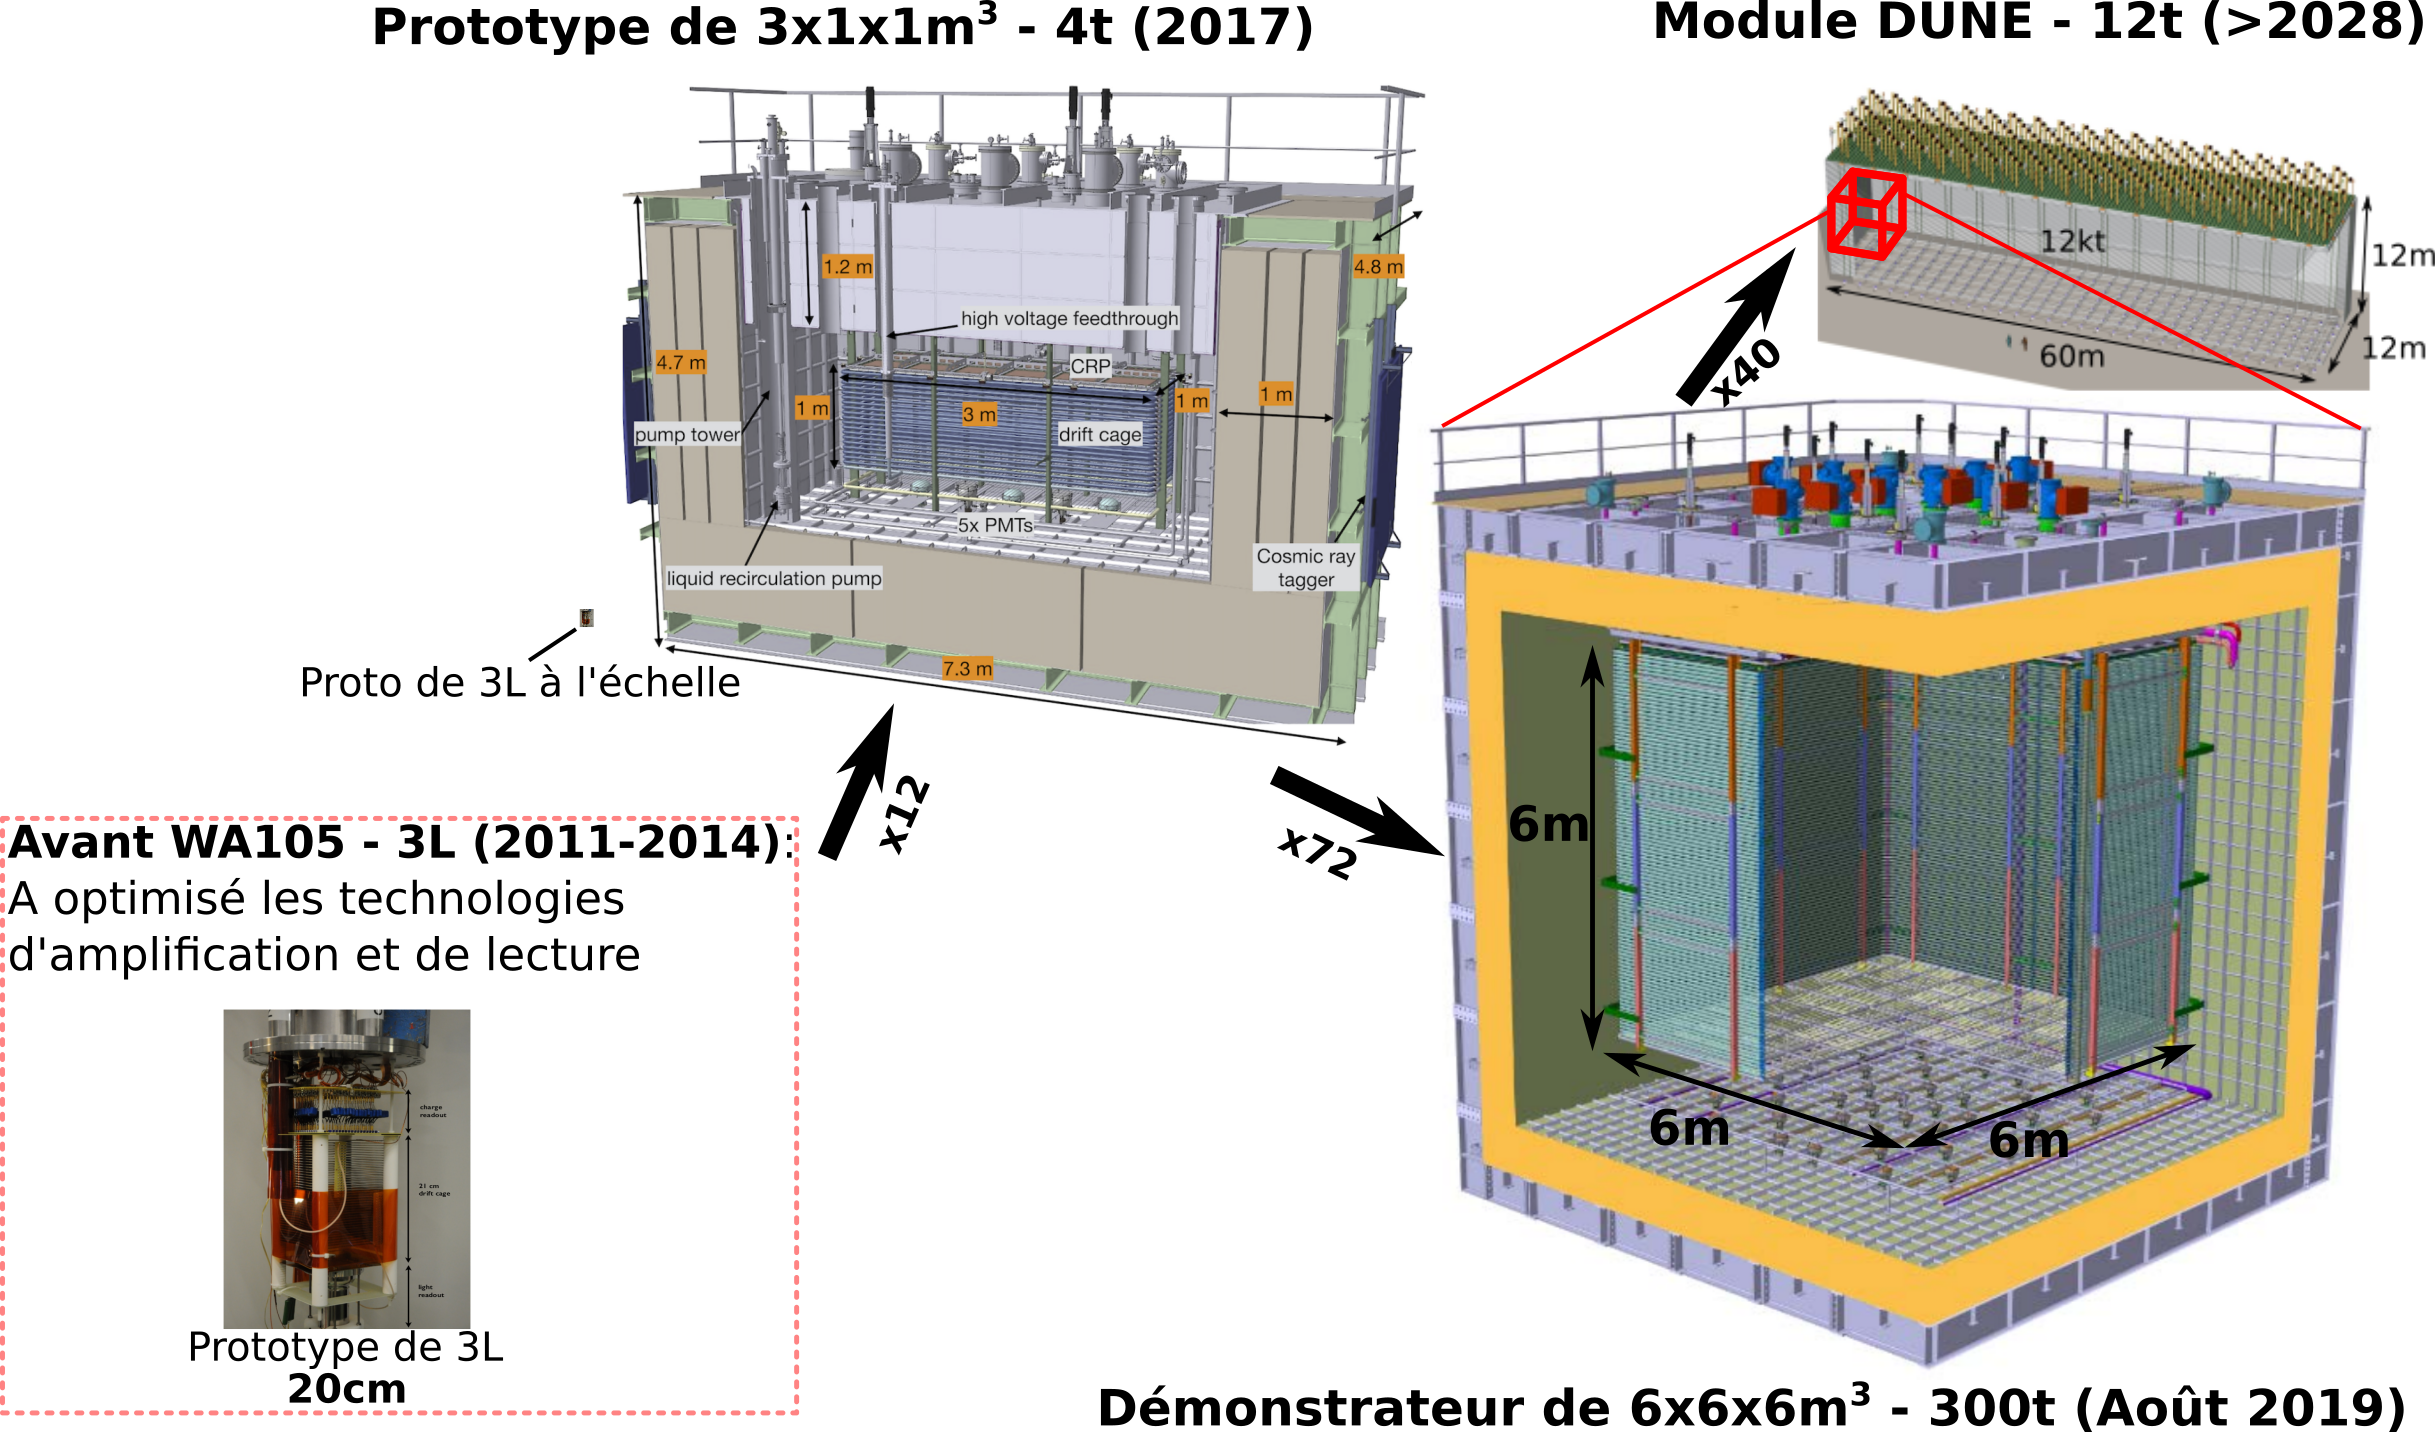
\includegraphics[width=1.03\linewidth]{wa105_scales.pdf}
    \end{frame}
        
    \begin{frame}{Le CRP}{Plan de lecture de charge}
   		\begin{minipage}{0.43\textwidth}
   			\begin{scriptsize}
	   			\textbf{Gain effectif (avalanche de Townsend):}\\
	   		\end{scriptsize}
   			$G_{eff} = \mathcal{T}e^{A\rho d e^{-B\rho d/V}}$\\
   			\begin{scriptsize}
    			\begin{itemize}
    				\item $\mathcal{T}$: Transparence aux électrons
    				\item $A,B$: coefficients, dépendent du gaz
    				\item $d$: distance d'amplification (\SI{1}{\milli\meter})
    				\item $V$: tension d'amplification ($\sim$\SI{3}{\kilo\volt})
    				\item $\rho$: densité du gaz ($\propto P/T$)
    			\end{itemize}
    		\end{scriptsize} 
   			\vfill\centering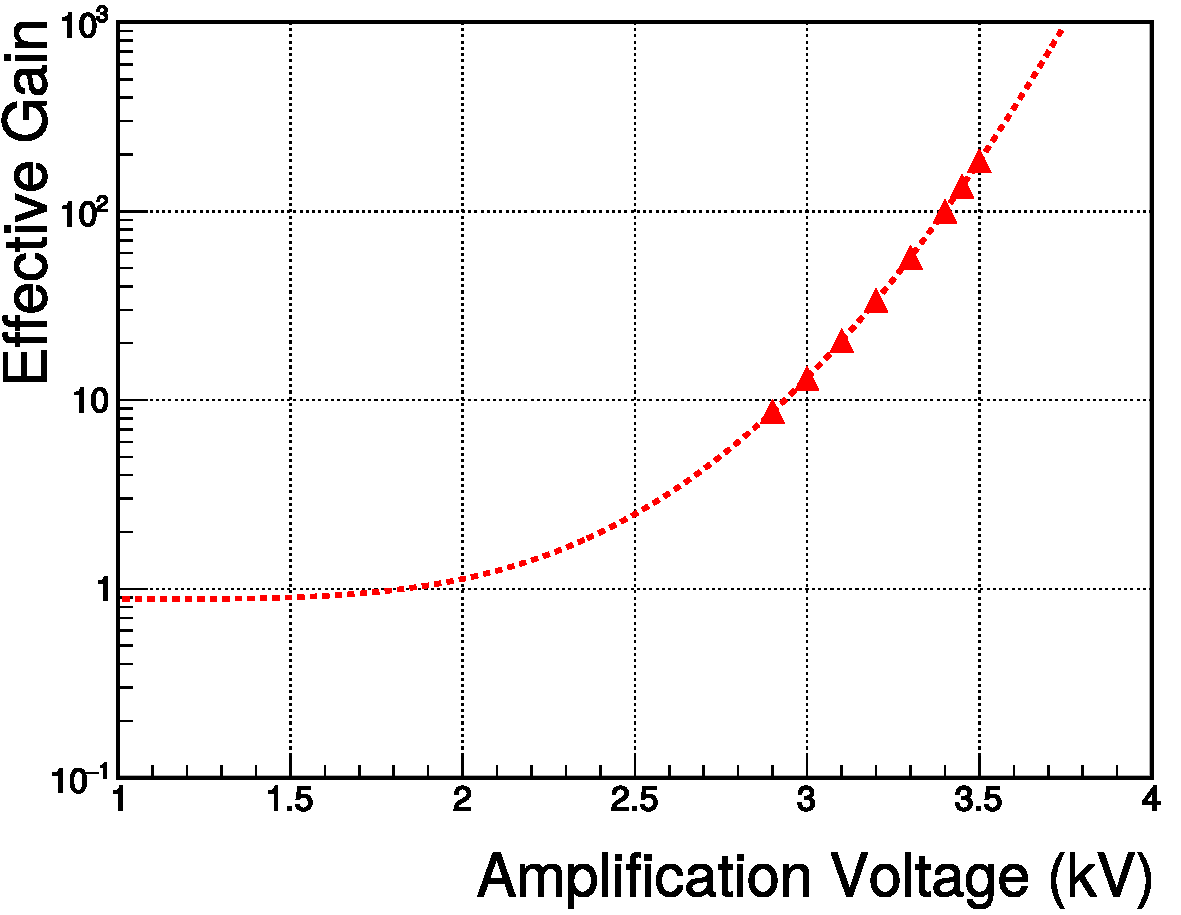
\includegraphics[width=0.8\textwidth]{./pictures/gain_3L.pdf}\\\tiny{C. Cantini et al., 2014, doi : 10.1088/1748-0221/10/03/P03017}
   		\end{minipage}\hfill
   		\begin{minipage}{0.52\textwidth}
   			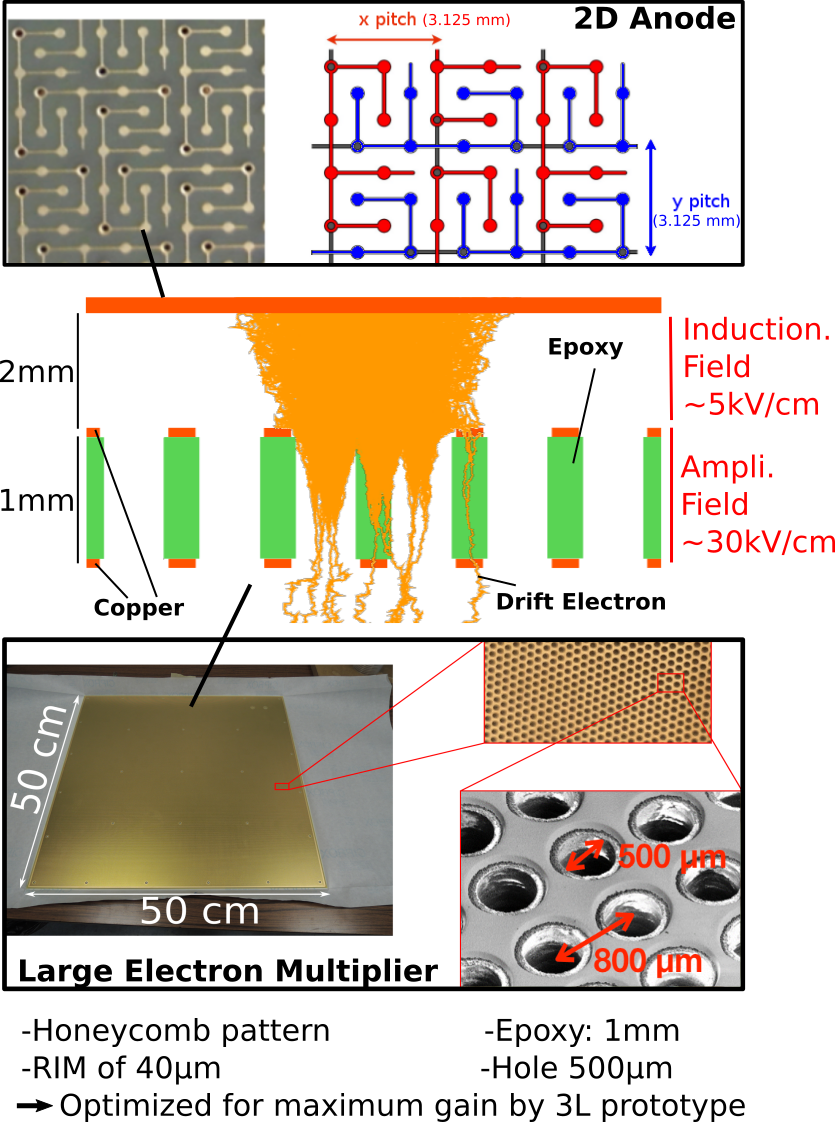
\includegraphics[width=\textwidth]{lem_anode.pdf}
   		\end{minipage}
    \end{frame}
    
    \begin{frame}{Les LEMs}{Où se passe l'amplification}
        \begin{scriptsize}
            \centering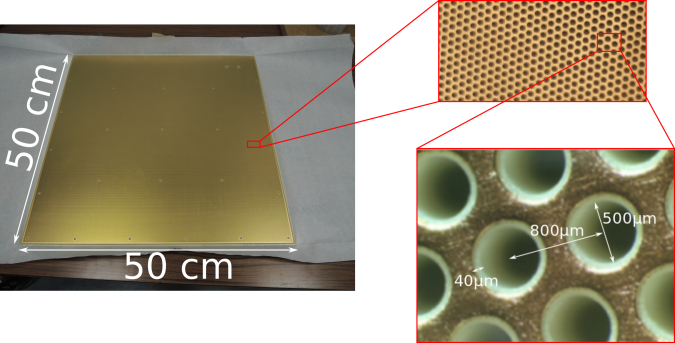
\includegraphics[width=\textwidth]{LEM_zoom.png}
            \begin{columns}
                \begin{column}{0.5\textwidth}
                    \centering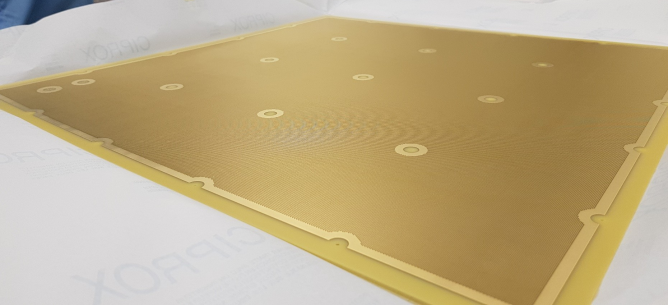
\includegraphics[width=0.8\textwidth]{./pictures/LEM.png}
                \end{column}
                \begin{column}{0.5\textwidth}
                    \begin{itemize}
                        \item PCB (epoxy FR4) recouvert de cuivre
                        \item 50$\times$\SI{50}{\centi\meter\squared}
                        \item \SI{1}{\milli\meter} d'épaisseur
                        \item 400k trous
                        \item Bords = zones sans trous
                    \end{itemize}
                \end{column}
            \end{columns}
        \end{scriptsize}
    \end{frame}
    
    \begin{frame}{Le charging up}{Accumulation d'électrons sur le FR4}
        \begin{scriptsize}
            \begin{columns}
       			\begin{column}{0.5\textwidth}
           			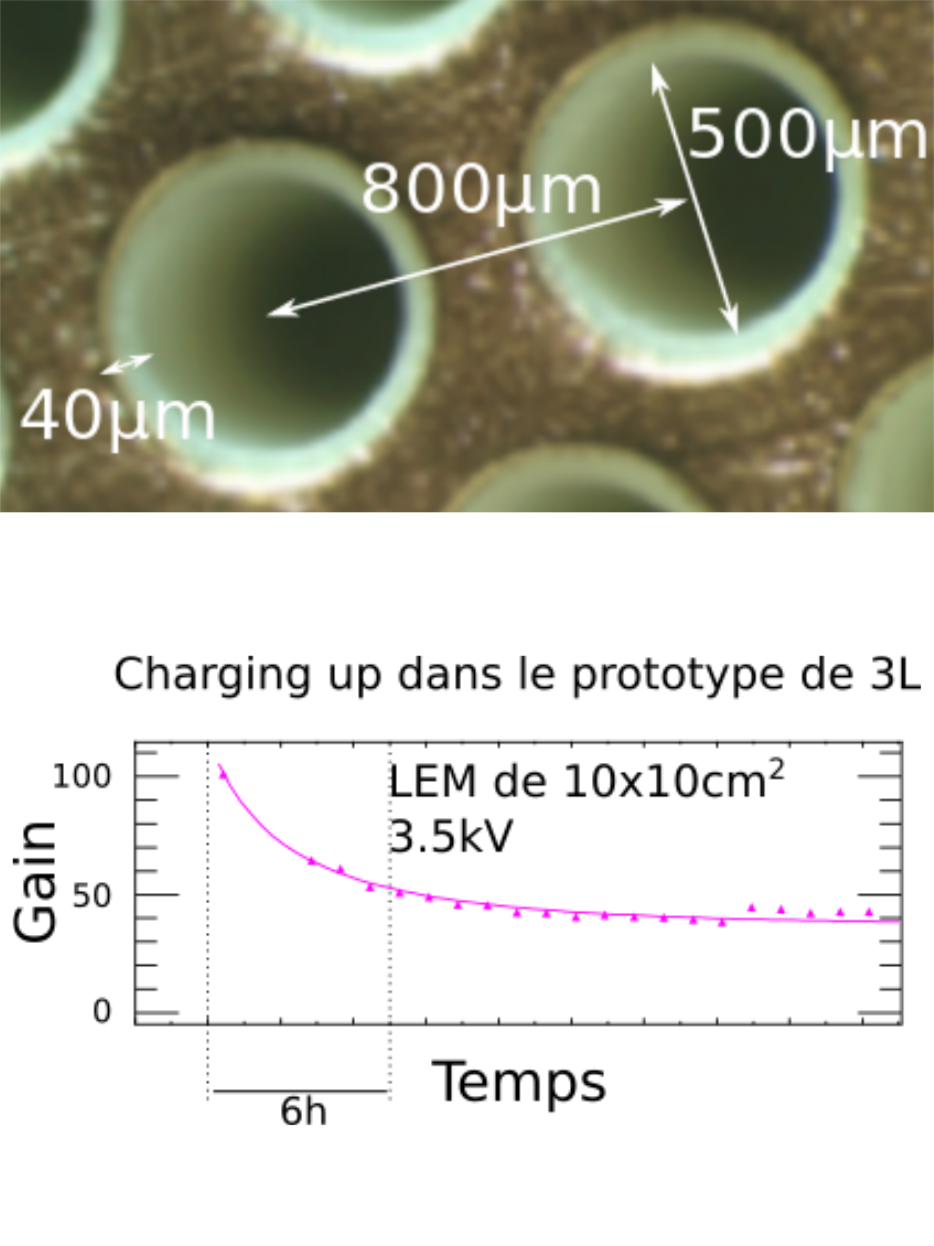
\includegraphics[width=\textwidth]{CU_time.png}
       			\end{column}\hfill
       			\begin{column}{0.5\textwidth}
       				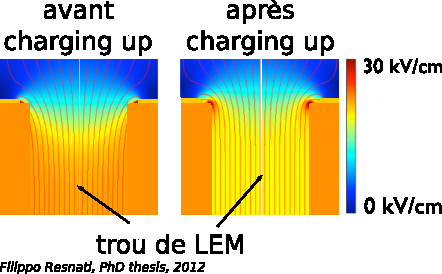
\includegraphics[width=\textwidth]{CU.pdf}\\\vspace{1cm}
           			\textbf{Rim autour des trous :}
       				\begin{itemize}
       					\item[$\Rightarrow$] Lignes de champ traversent le FR4\\
       					\item[$\Rightarrow$] L'accumulation d'électron sur le FR4 \textcolor{blue}{déforme et atténue} le champ
%    					\item Le temps de charging up time dépend de la tension dans le LEM et du taux de dépôt de charge.
       				\end{itemize}
       				Charging up: \textcolor{red}{$G_{eff}(t)$ décroît} jusqu'à un plateau.
           		\end{column}
           	\end{columns}
        \end{scriptsize}
    \end{frame}
        
        \begin{frame}{Le charging up}{Accumulation d'électrons sur le FR4}
            \begin{scriptsize}
                \begin{columns}
           			\begin{column}{0.5\textwidth}
               			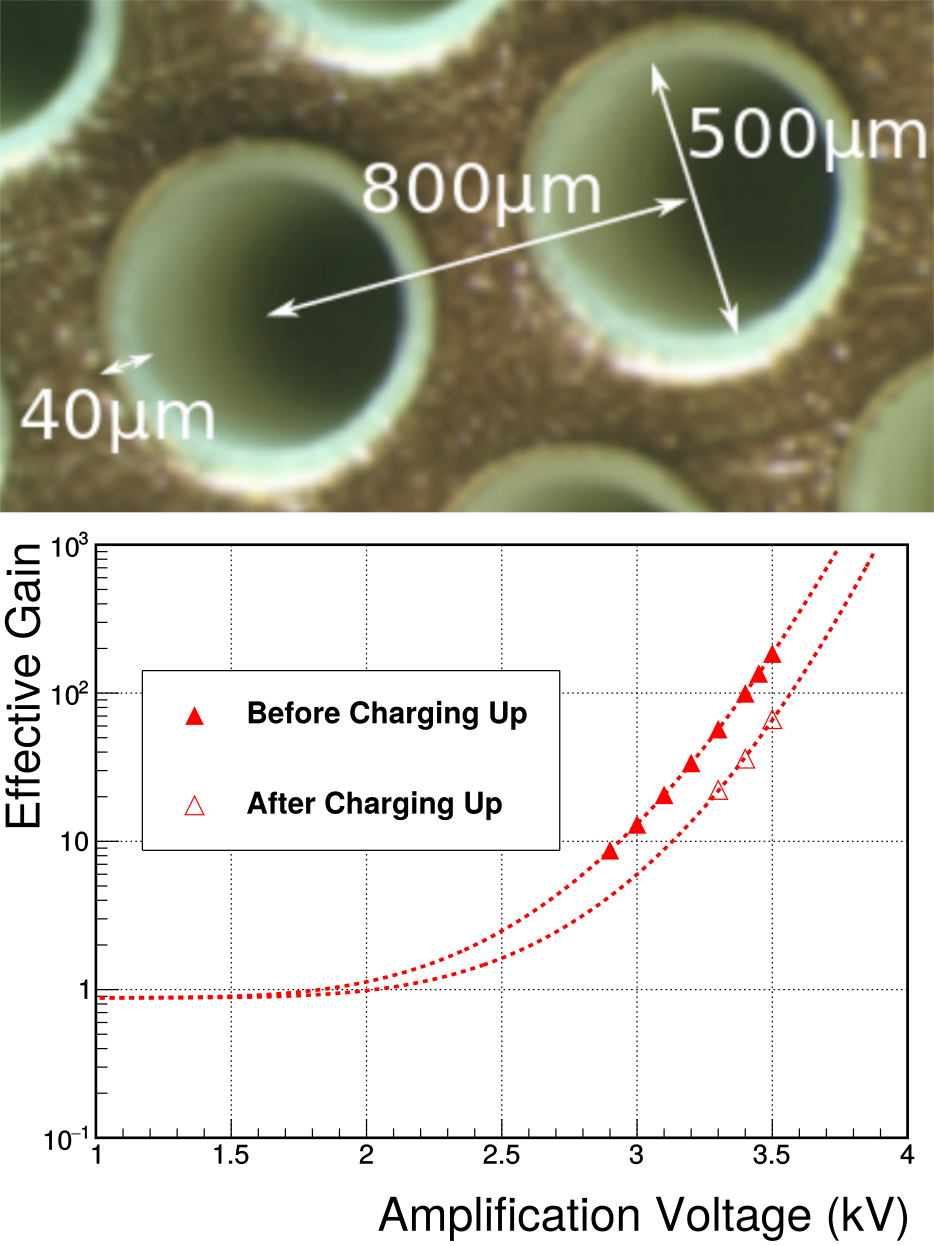
\includegraphics[width=\textwidth]{CU_ampli.png}
           			\end{column}\hfill
           			\begin{column}{0.5\textwidth}
           				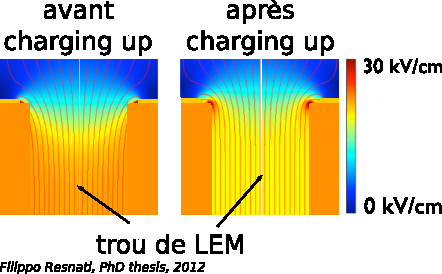
\includegraphics[width=\textwidth]{CU.pdf}\\\vspace{1cm}
               			\textbf{Rim autour des trous :}
           				\begin{itemize}
           					\item[$\Rightarrow$] Lignes de champ traversent le FR4\\
           					\item[$\Rightarrow$] L'accumulation d'électron sur le FR4 \textcolor{blue}{déforme et atténue} le champ
    %    					\item Le temps de charging up time dépend de la tension dans le LEM et du taux de dépôt de charge.
           				\end{itemize}
           				Charging up: \textcolor{red}{$G_{eff}(t)$ décroît} jusqu'à un plateau.
               		\end{column}
               	\end{columns}
            \end{scriptsize}
        \end{frame}

%  {
%    	\setlength\pdfpagewidth{12.8cm}%
%    	\setlength\pdfpageheight{9.15cm}%
%    	\usebackgroundtemplate{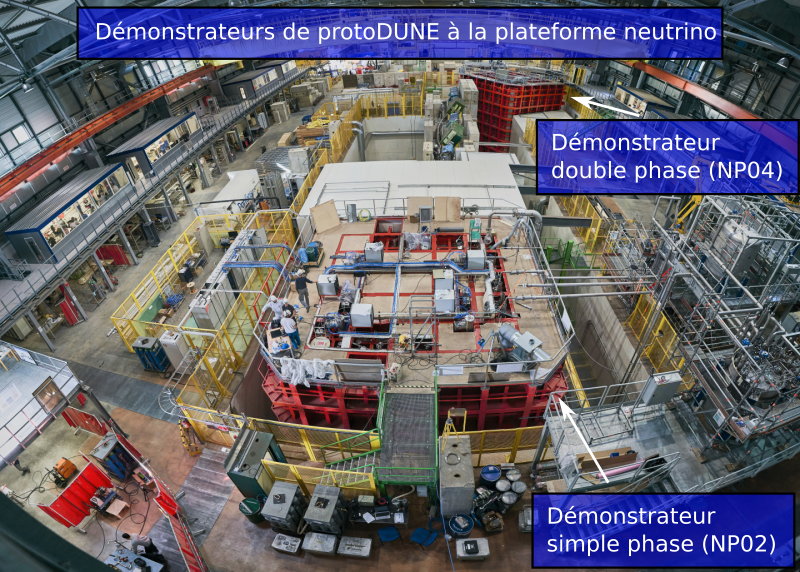
\includegraphics[width=\paperwidth]{nu_platform.png}}
%    	\begin{frame}[plain]
%    	\end{frame}
%    }
    
    
    \section[\TOO{}]{Analyse des données et simulations du prototype de DLArTPC de \TOO{}}
    
    {
       	\usebackgroundtemplate{
\includegraphics[width=\paperwidth]{./pictures/1.pdf}}
        \begin{specialframe}
            \vspace{2cm}\hspace*{-1.8cm}\parbox[t]{\textwidth}{
                \begin{center}
                    \begin{huge}
                            \textcolor{pheniics_purple}{\textbf{Analyse des données et simulations du prototype de \TOO{}}}
                    \end{huge}
                    \vspace{1cm}
                    \begin{itemize}
                        \item Présentation du prototype et principaux résultats
                        \item Analyse du gain effectif et simulations
                        \item Reconstruction de traces à bas champ d'extraction
                    \end{itemize}
                \end{center}
            }
        \end{specialframe}
    }
   
    \begin{frame}{Le prototype de \TOO{}}
   		\begin{scriptsize}
        	\centering
        	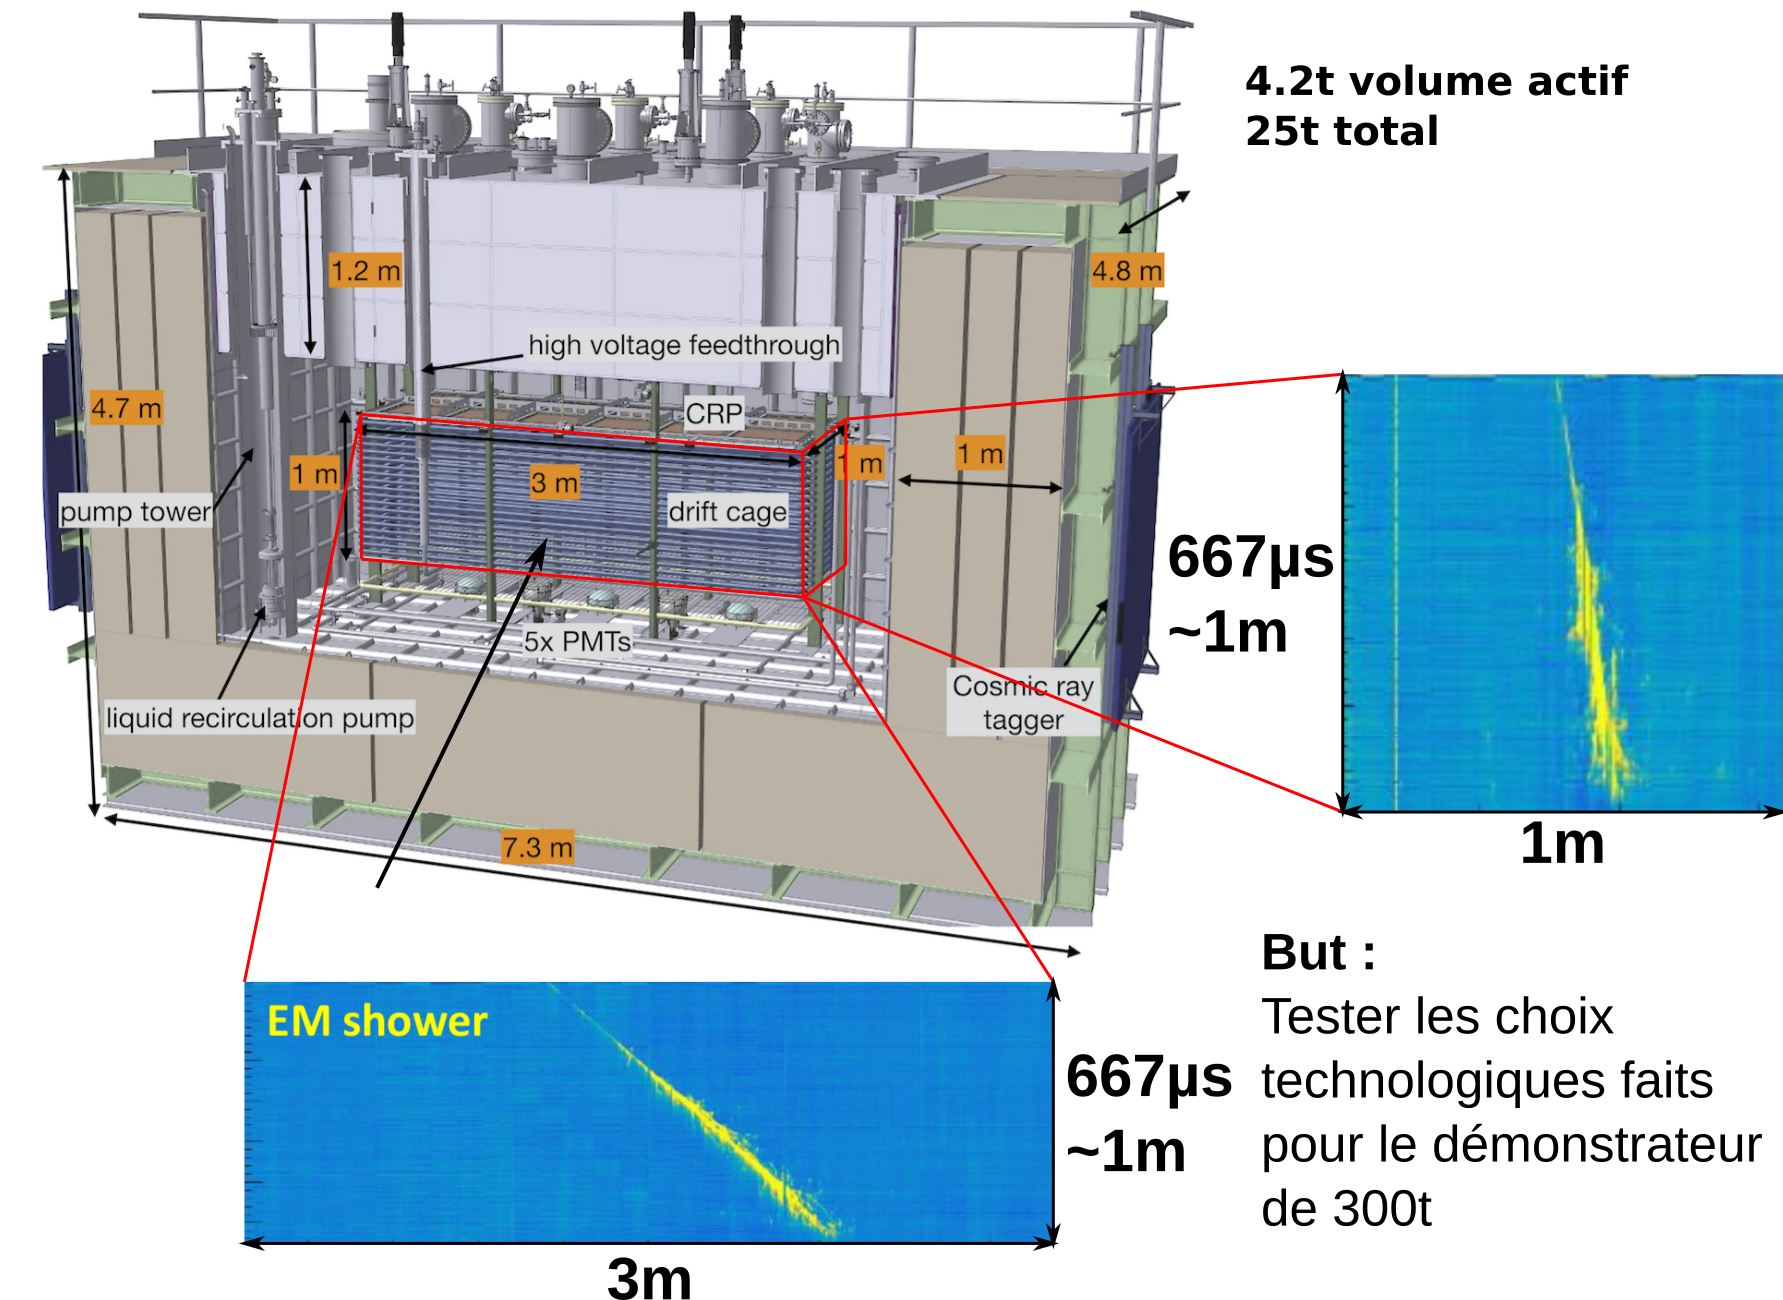
\includegraphics[width=\textwidth]{./pictures/311_2.png}        	
		\end{scriptsize}
   	\end{frame}
   	
   	\begin{frame}{Le prototype de \TOO{}}{Principaux résultats}
       	\begin{scriptsize}
           	\begin{columns}
               	\begin{column}{0.5\textwidth}
                   	\textbf{Construit en 2016--2017, opéré entre Juin et Novembre 2017, Publication en 2018}\\
       	           	\begin{itemize}
           	           	\item Fonctionnement d'une DLArTPC de \SI{4}{\tonne} : \textcolor{green}{\checkmark}
       	               	\item Champs stables (10h):
       	               	\begin{itemize}\begin{scriptsize}
       	                   	\item Extraction (liquide) \SI{1.9}{\kilo\volt\per\centi\meter}
       	                   	\item Amplification \SI{28}{\kilo\volt\per\centi\meter}
       	                   	\item Induction \SI{1.5}{\kilo\volt\per\centi\meter}\end{scriptsize}
       	               	\end{itemize}
       	               	\item Impuretés $<\SI{75}{ppt}$ equiv. $O_2$ : \textcolor{green}{\checkmark}
       	               	\item Scintillation clairement détectée : \textcolor{green}{\checkmark}
       	           	\end{itemize}
       	           	\hspace{-0.3cm}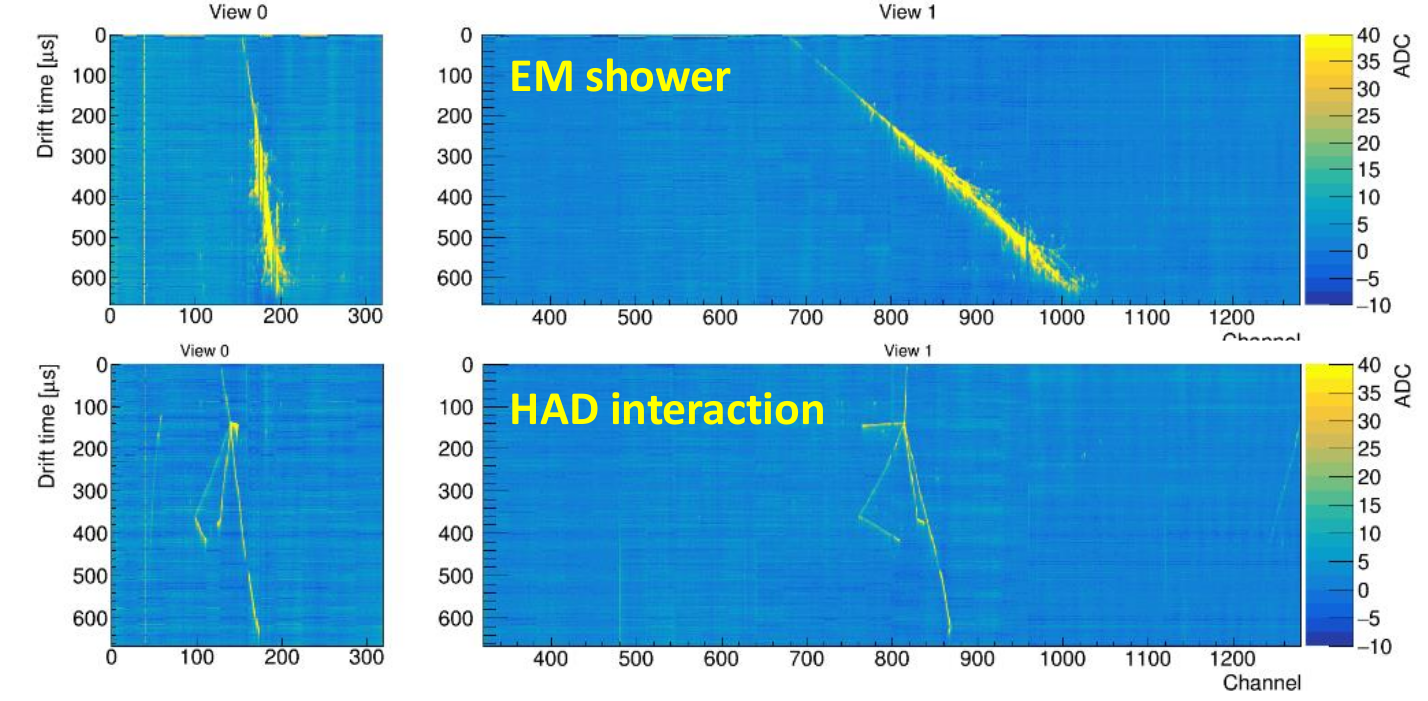
\includegraphics[width=1.2\textwidth]{./pictures/events.png}
               	\end{column}
               	\begin{column}{0.5\textwidth}
                   	\flushright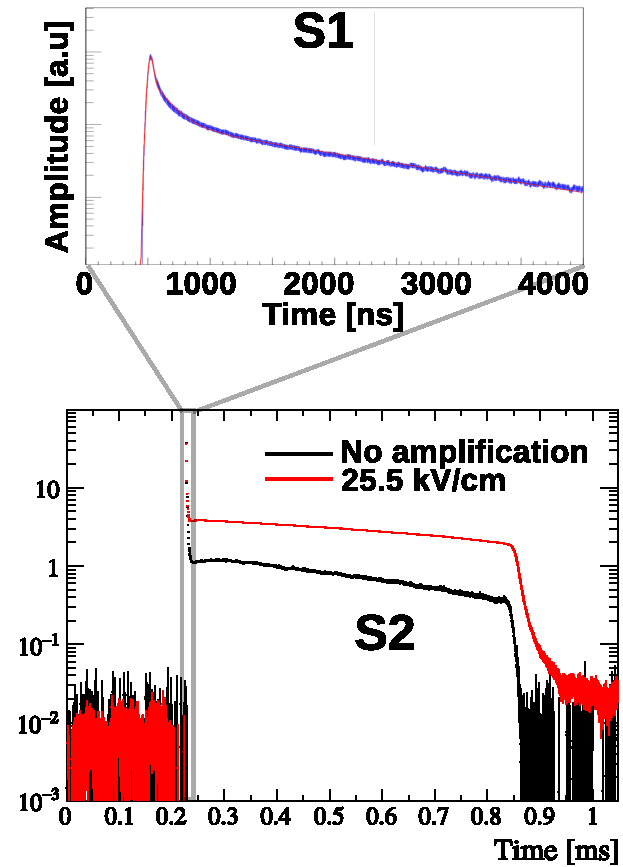
\includegraphics[width=0.95\textwidth]{./pictures/scintillation.pdf}
               	\end{column}
           	\end{columns}
       	\end{scriptsize}
   	\end{frame}
   	
   	\subsection{Méthode d'analyse}
	    
    \begin{frame}{Le prototype de \TOO{}}{L'analyse}
       	\begin{scriptsize}
       		\vfill
       		\begin{columns}
       			\begin{column}{0.32\textwidth}
       				\textbf{Difficultés rencontrées:} 
       				\begin{itemize}
       					\item \textcolor{red}{Grille limitée} à \SI{5}{\kilo\volt} (nominale : \SI{7}{\kilo\volt})
       					\item \textcolor{red}{Instabilité} à haute tension à travers les LEMs
       					\item \textcolor{red}{Déformation du CRP} $\sim\SI{3}{\milli\meter}$
       				\end{itemize}
       				\textbf{$\Rightarrow$ Améliorations apportées dans le \SSS{}} \\
       				\vspace{0.3cm}
       				\textbf{Analyse principale :} Gain
       				\begin{itemize}
           				\item vs champ d'amplification
           				\item vs champ d'extraction
           				\item vs temps
           				\item à travers le CRP
       				\end{itemize}
       				$\Rightarrow$ Utilise les muons cosmiques (MIP)
       			\end{column}\hfill
       			\begin{column}{0.72\textwidth}
       				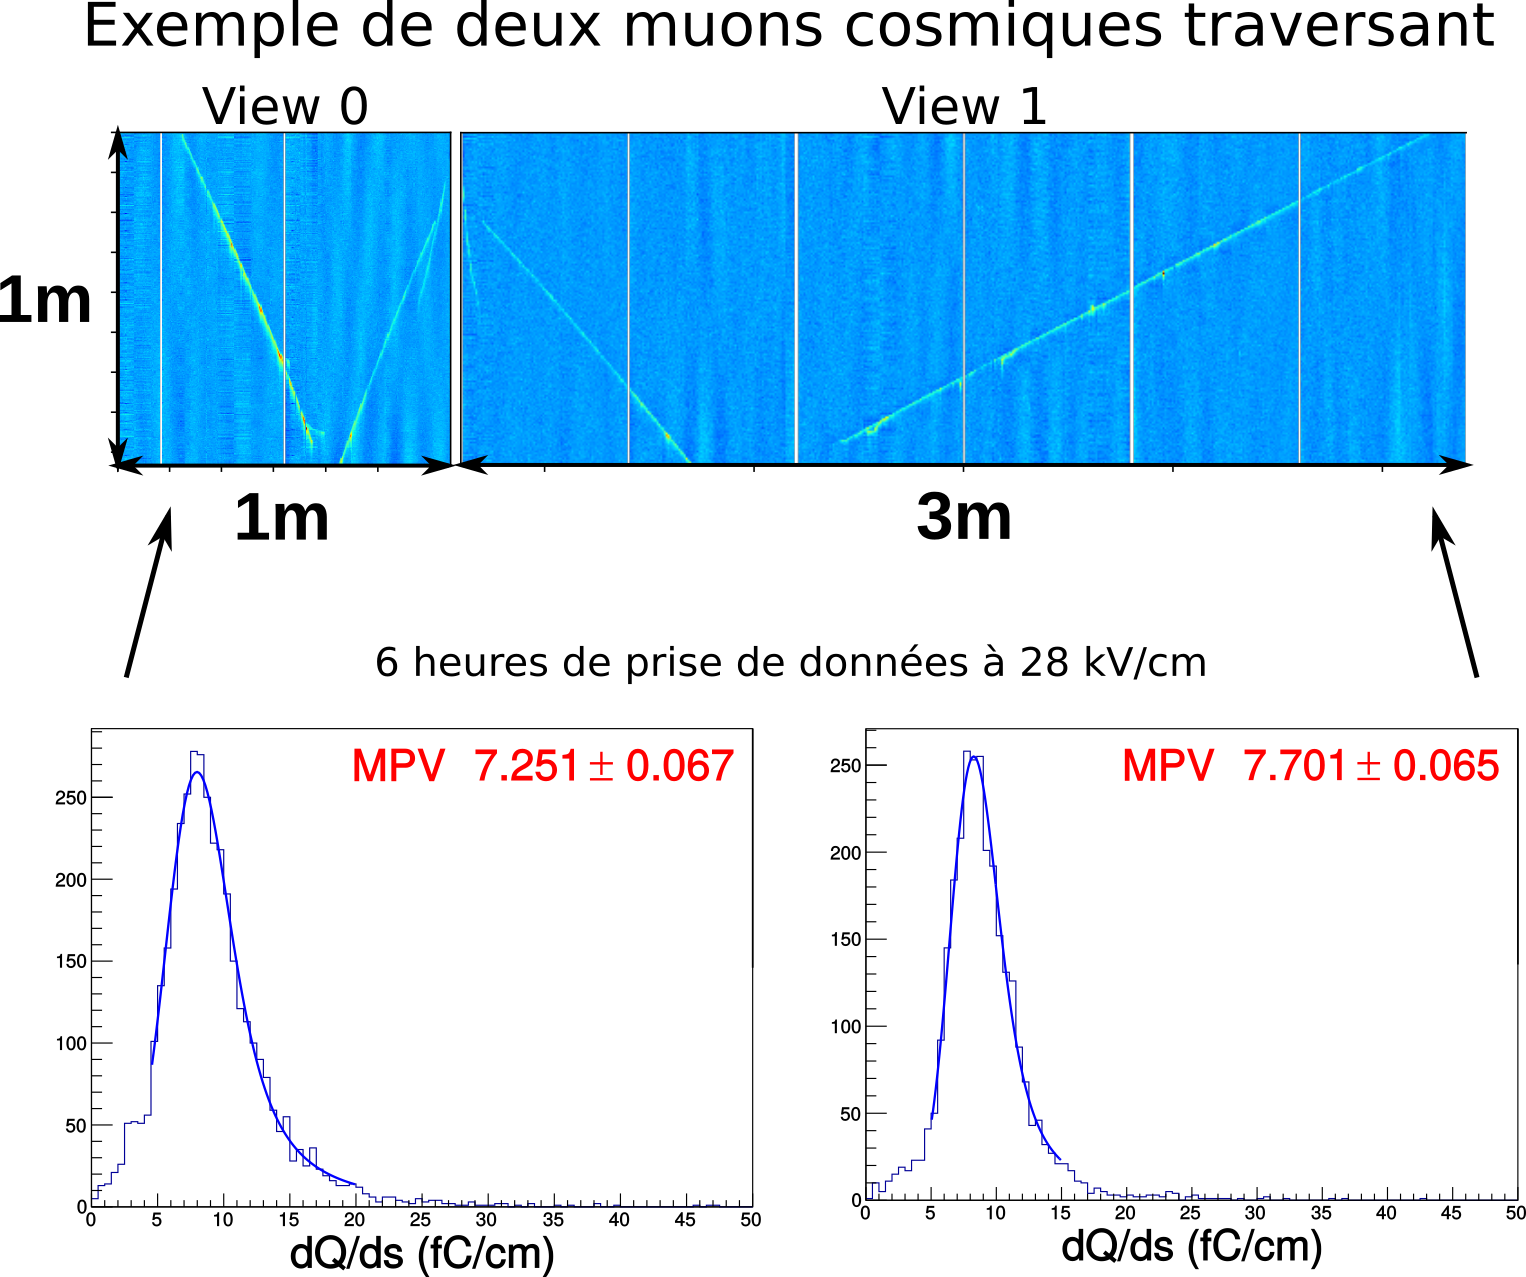
\includegraphics[width=\textwidth]{./pictures/run840.png}\\
       			\end{column}
       		\end{columns}
	    \end{scriptsize}
    \end{frame}

    
    \begin{frame}{Le prototype de \TOO{}}{L'analyse}
        \begin{scriptsize}
       		\vfill
       		\begin{columns}
       			\begin{column}{0.32\textwidth}
           			\textbf{Prochaines sections :}
       				\begin{enumerate}
                        \item Méthode d'analyse
                        \item Efficacités de collection
                        \item Principales incertitudes
                        \item Simulations : zones mortes
                        \item Charging up
                        \item Gain vs Amplification
                        \item Reconstruction à basse extraction
                    \end{enumerate}
       			\end{column}\hfill
       			\begin{column}{0.72\textwidth}
       				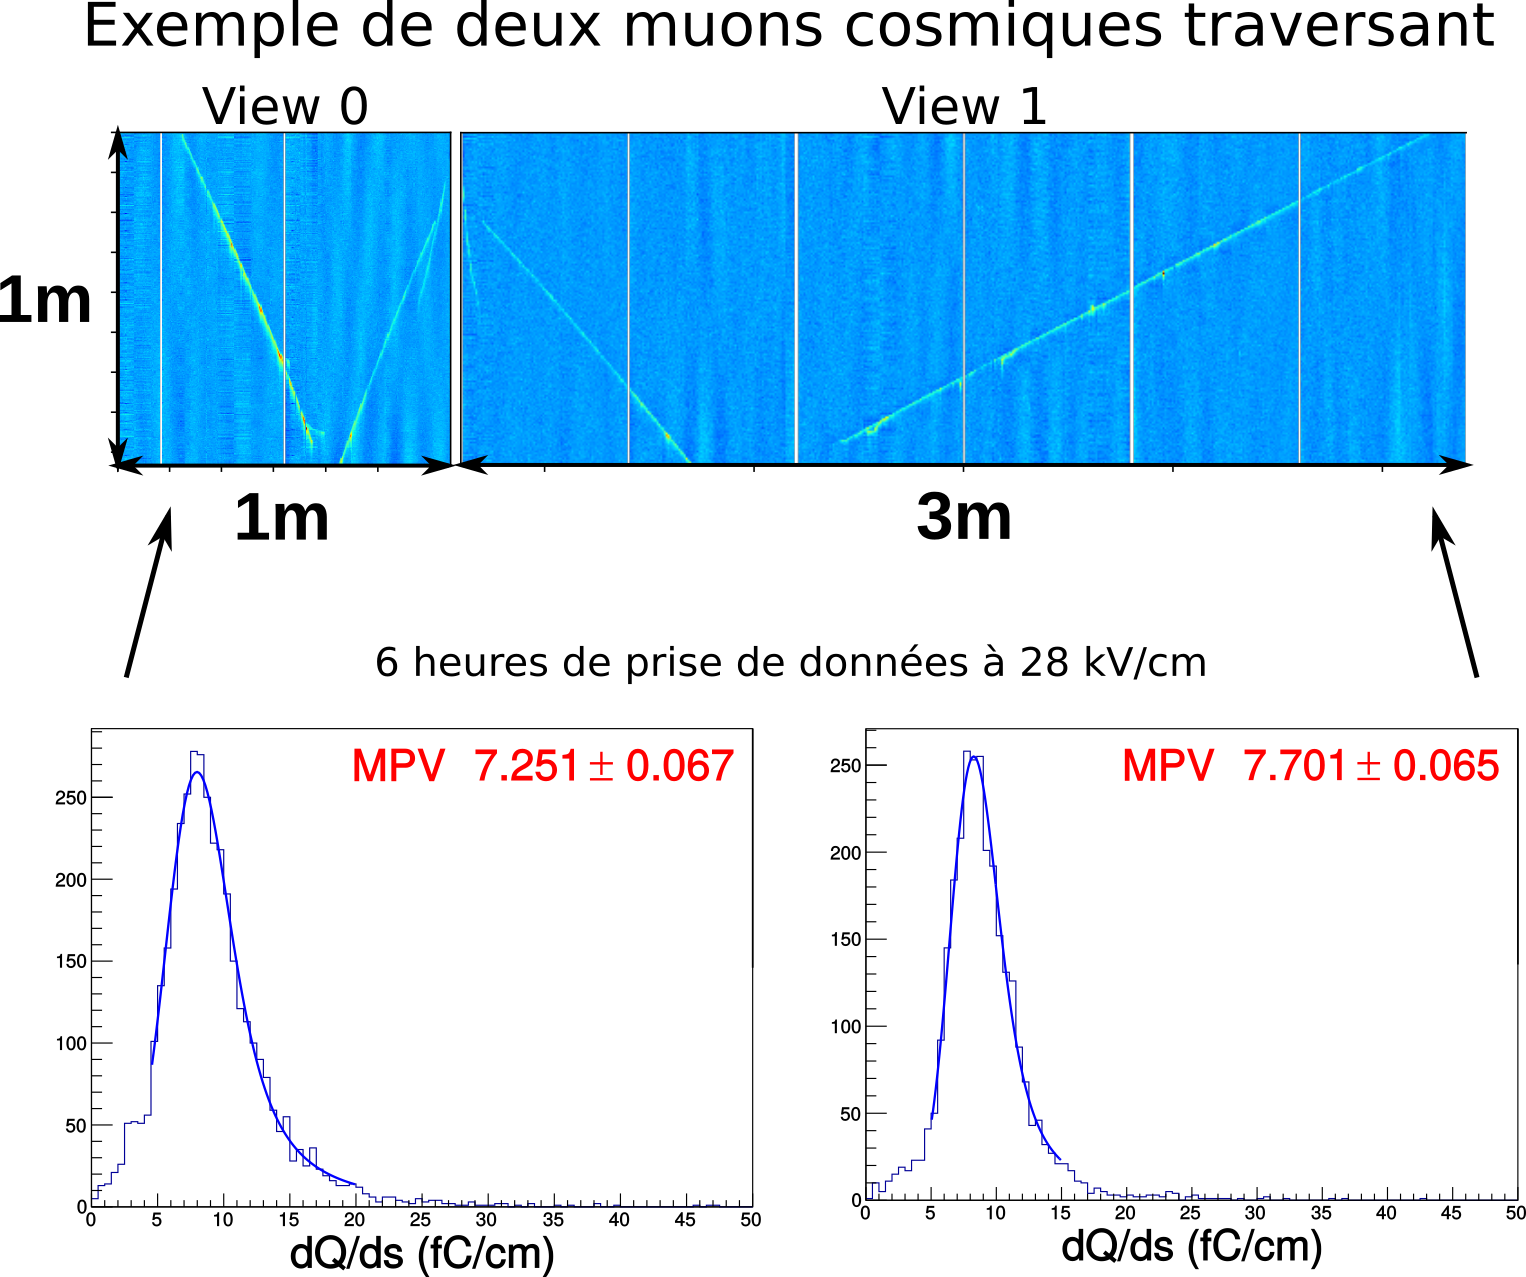
\includegraphics[width=\textwidth]{./pictures/run840.png}\\
       			\end{column}
       		\end{columns}
\end{scriptsize}
    \end{frame}

    \begin{frame}{Mesure du gain avec des muons cosmiques}{Distribution de Landau-Vavilov}
       	\begin{scriptsize}
            \begin{columns}
                \begin{column}{0.6\textwidth}
                    \centering 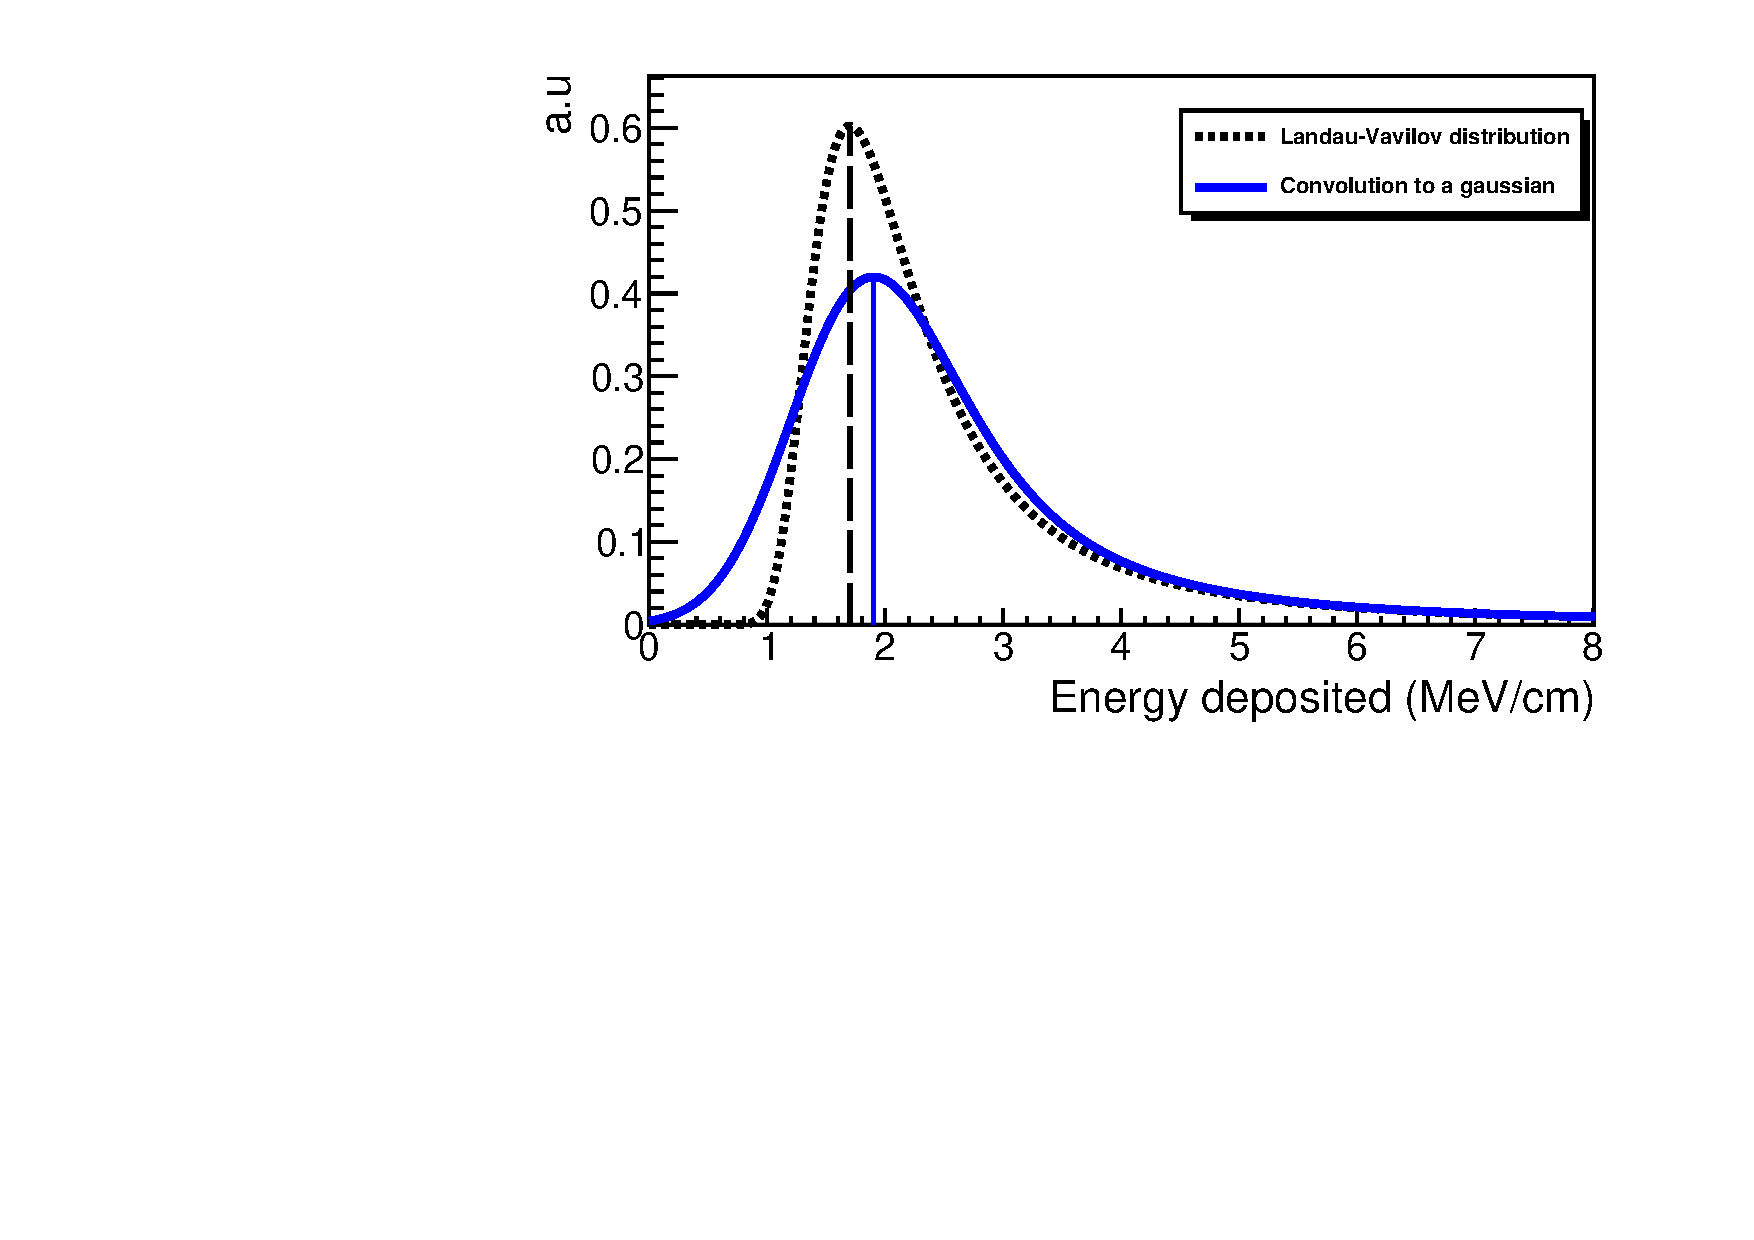
\includegraphics[width=\textwidth]{langau.pdf}
                \end{column}\hfill
                \begin{column}{0.4\textwidth}
                    \begin{itemize}
          					\item Muon cosmique : MIP \\ $\Rightarrow$ dépôt d'énergie attendu connu
          					\item Valeur la plus probable (MPV) = \SI{1.7}{\mega\electronvolt\per\centi\meter}
          					\item Après recombinaison avec les ions (loi de Birks) : \textcolor{red}{\SI{8.26}{\femto\coulomb\per\centi\meter}}
          					\item $G_{eff}=\frac{MPV_0 + MPV_1}{MPV_{attendue}}$
          				\end{itemize}
                \end{column}
            \end{columns}
            \vspace{0.2cm}
            Calibration de l'électronique du \TOO{} $\Rightarrow$ conversion ADC$\times$temps$\to$\si{\femto\coulomb}
            \begin{center} 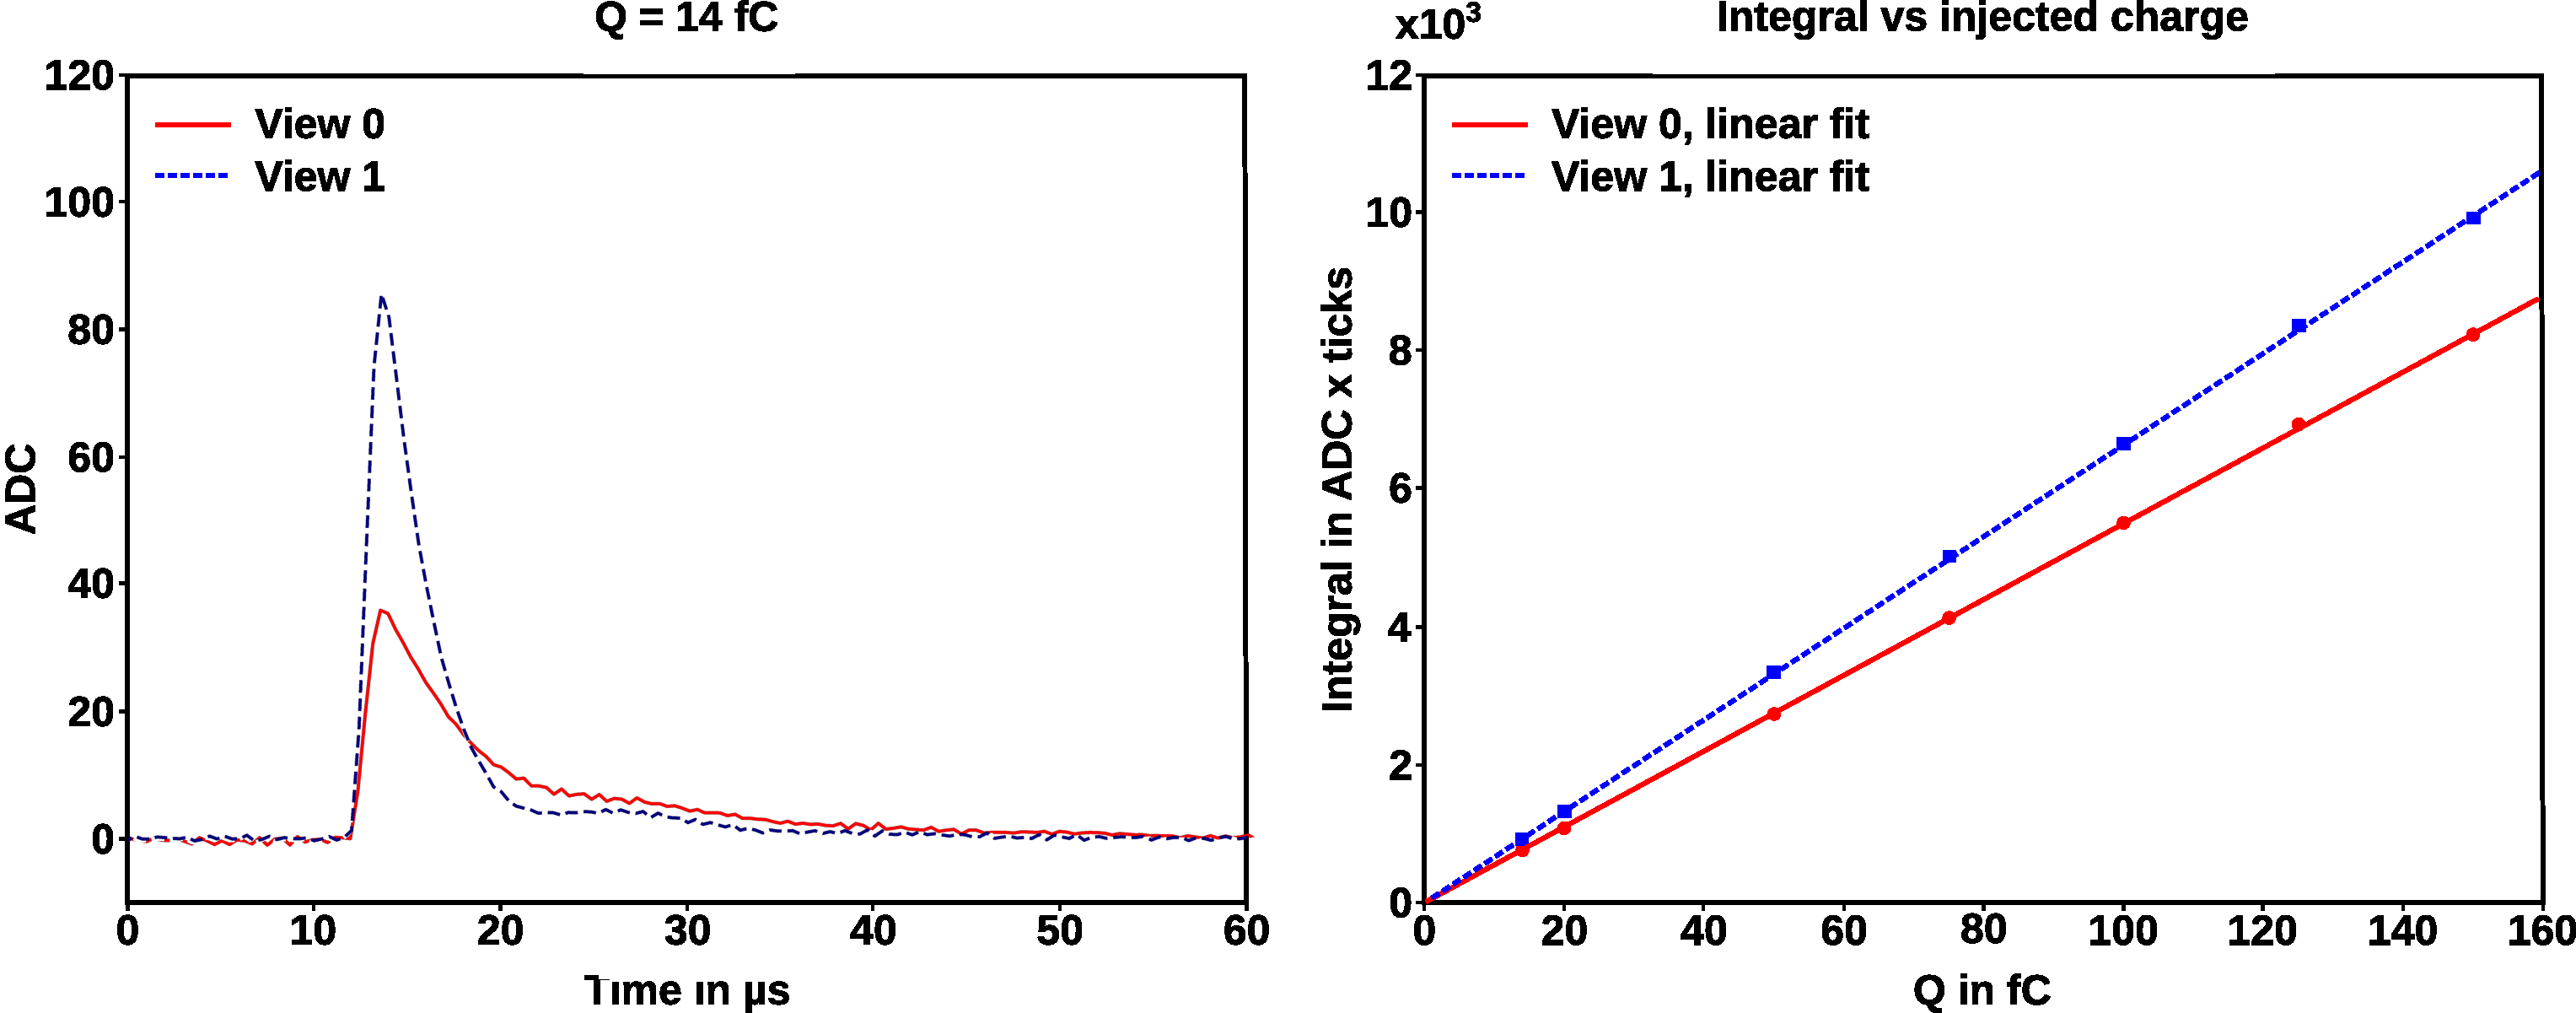
\includegraphics[width=0.8\textwidth]{calibration.pdf} \end{center}
	    \end{scriptsize}
    \end{frame}

    \begin{frame}{Sélection des muons}{Algorithme \textit{Highway}}
        \begin{scriptsize}
        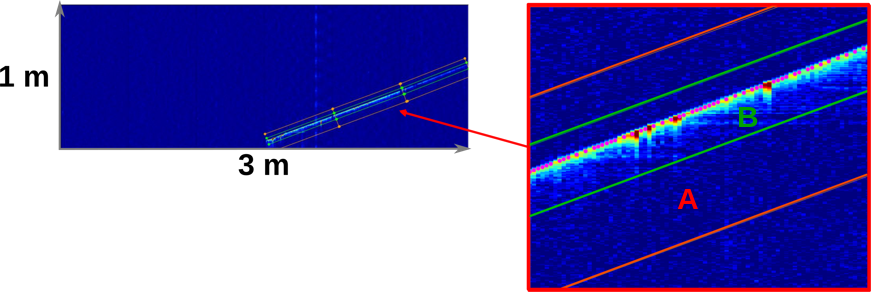
\includegraphics[width=\textwidth]{highway.png}
        \begin{columns}
            \begin{column}{0.5\textwidth}
                \begin{itemize}
                    \item Muon : trace longue, droite et nette \\ $\Rightarrow$ Coupure sur $\frac{Q_A-Q_B}{Q_A} < 0.1$
                    \item Coupures supplémentaires : \begin{itemize}\begin{scriptsize}\item longueur $>\SI{50}{\centi\meter}$. \item \SI{2}{\degree} autour de la verticale, de l'horizontale, et des directions parallèles aux canaux des anodes.\end{scriptsize}\end{itemize}
                \end{itemize}
            \end{column}
            \begin{column}{0.5\textwidth}
                \hspace{0.3cm} Simulation Monte Carlo :
                \begin{itemize}
                    \item Efficacité de sélection des muons : 68\,\%
                    \item Pureté : 92\,\% de muons
                \end{itemize}
            \end{column}
        \end{columns}
        \end{scriptsize}
    \end{frame}
    
    \begin{frame}{Avec un champ d'amplification de \SI{28}{\kilo\volt\per\centi\meter}}
        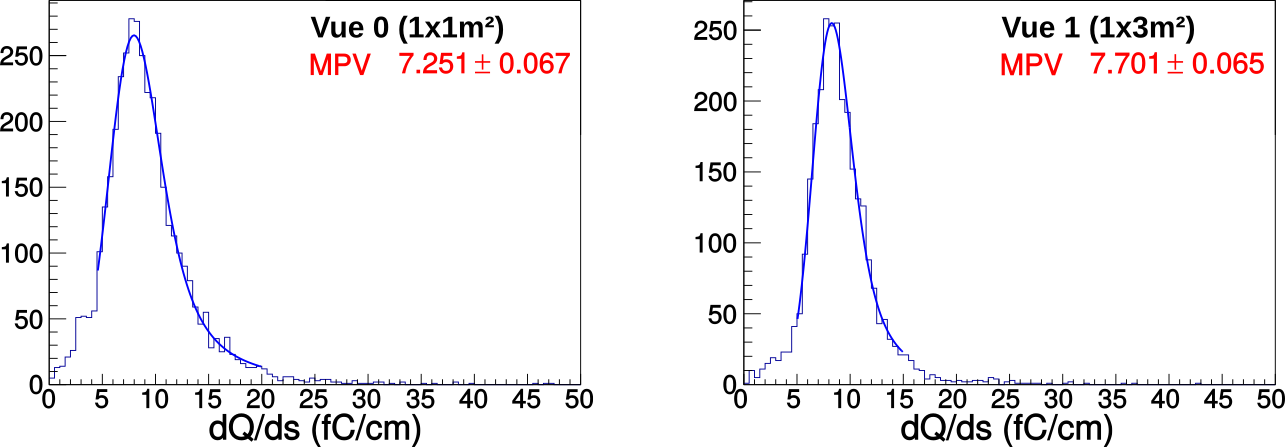
\includegraphics[width=\textwidth]{./pictures/dQds_840.png}\\\vfill
        \begin{columns}
            \begin{column}{0.55\textwidth}
                \begin{tabular}{l|l|l|}
                \cline{2-3}
                 & \SI{4}{\tonne} & \SI{3}{\liter} \\ \hline
                \multicolumn{1}{|l|}{$G_{eff}$} & 1.8 & 3.2 \\
                \multicolumn{1}{|l|}{$E_{extr}$} & \SI{1.9}{\kilo\volt\per\centi\meter} & \SI{2.5}{\kilo\volt\per\centi\meter} \\
                \multicolumn{1}{|l|}{$E_{ind}$} & \SI{1.5}{\kilo\volt\per\centi\meter} & \SI{5}{\kilo\volt\per\centi\meter} \\ \hline
                \end{tabular}
            \end{column}
            \begin{column}{0.45\textwidth}
                \begin{scriptsize}
                \TOO{} et \threeL{} : \textbf{Différents gains} et
                différents champs d'\textbf{extraction} et d'\textbf{induction}\\
                \end{scriptsize}
            \end{column}
        \end{columns}
    \end{frame}

    \subsection[Efficacités de collection]{Efficacités de collection}

    \begin{frame}{Efficacités de collection}{Simulation}
		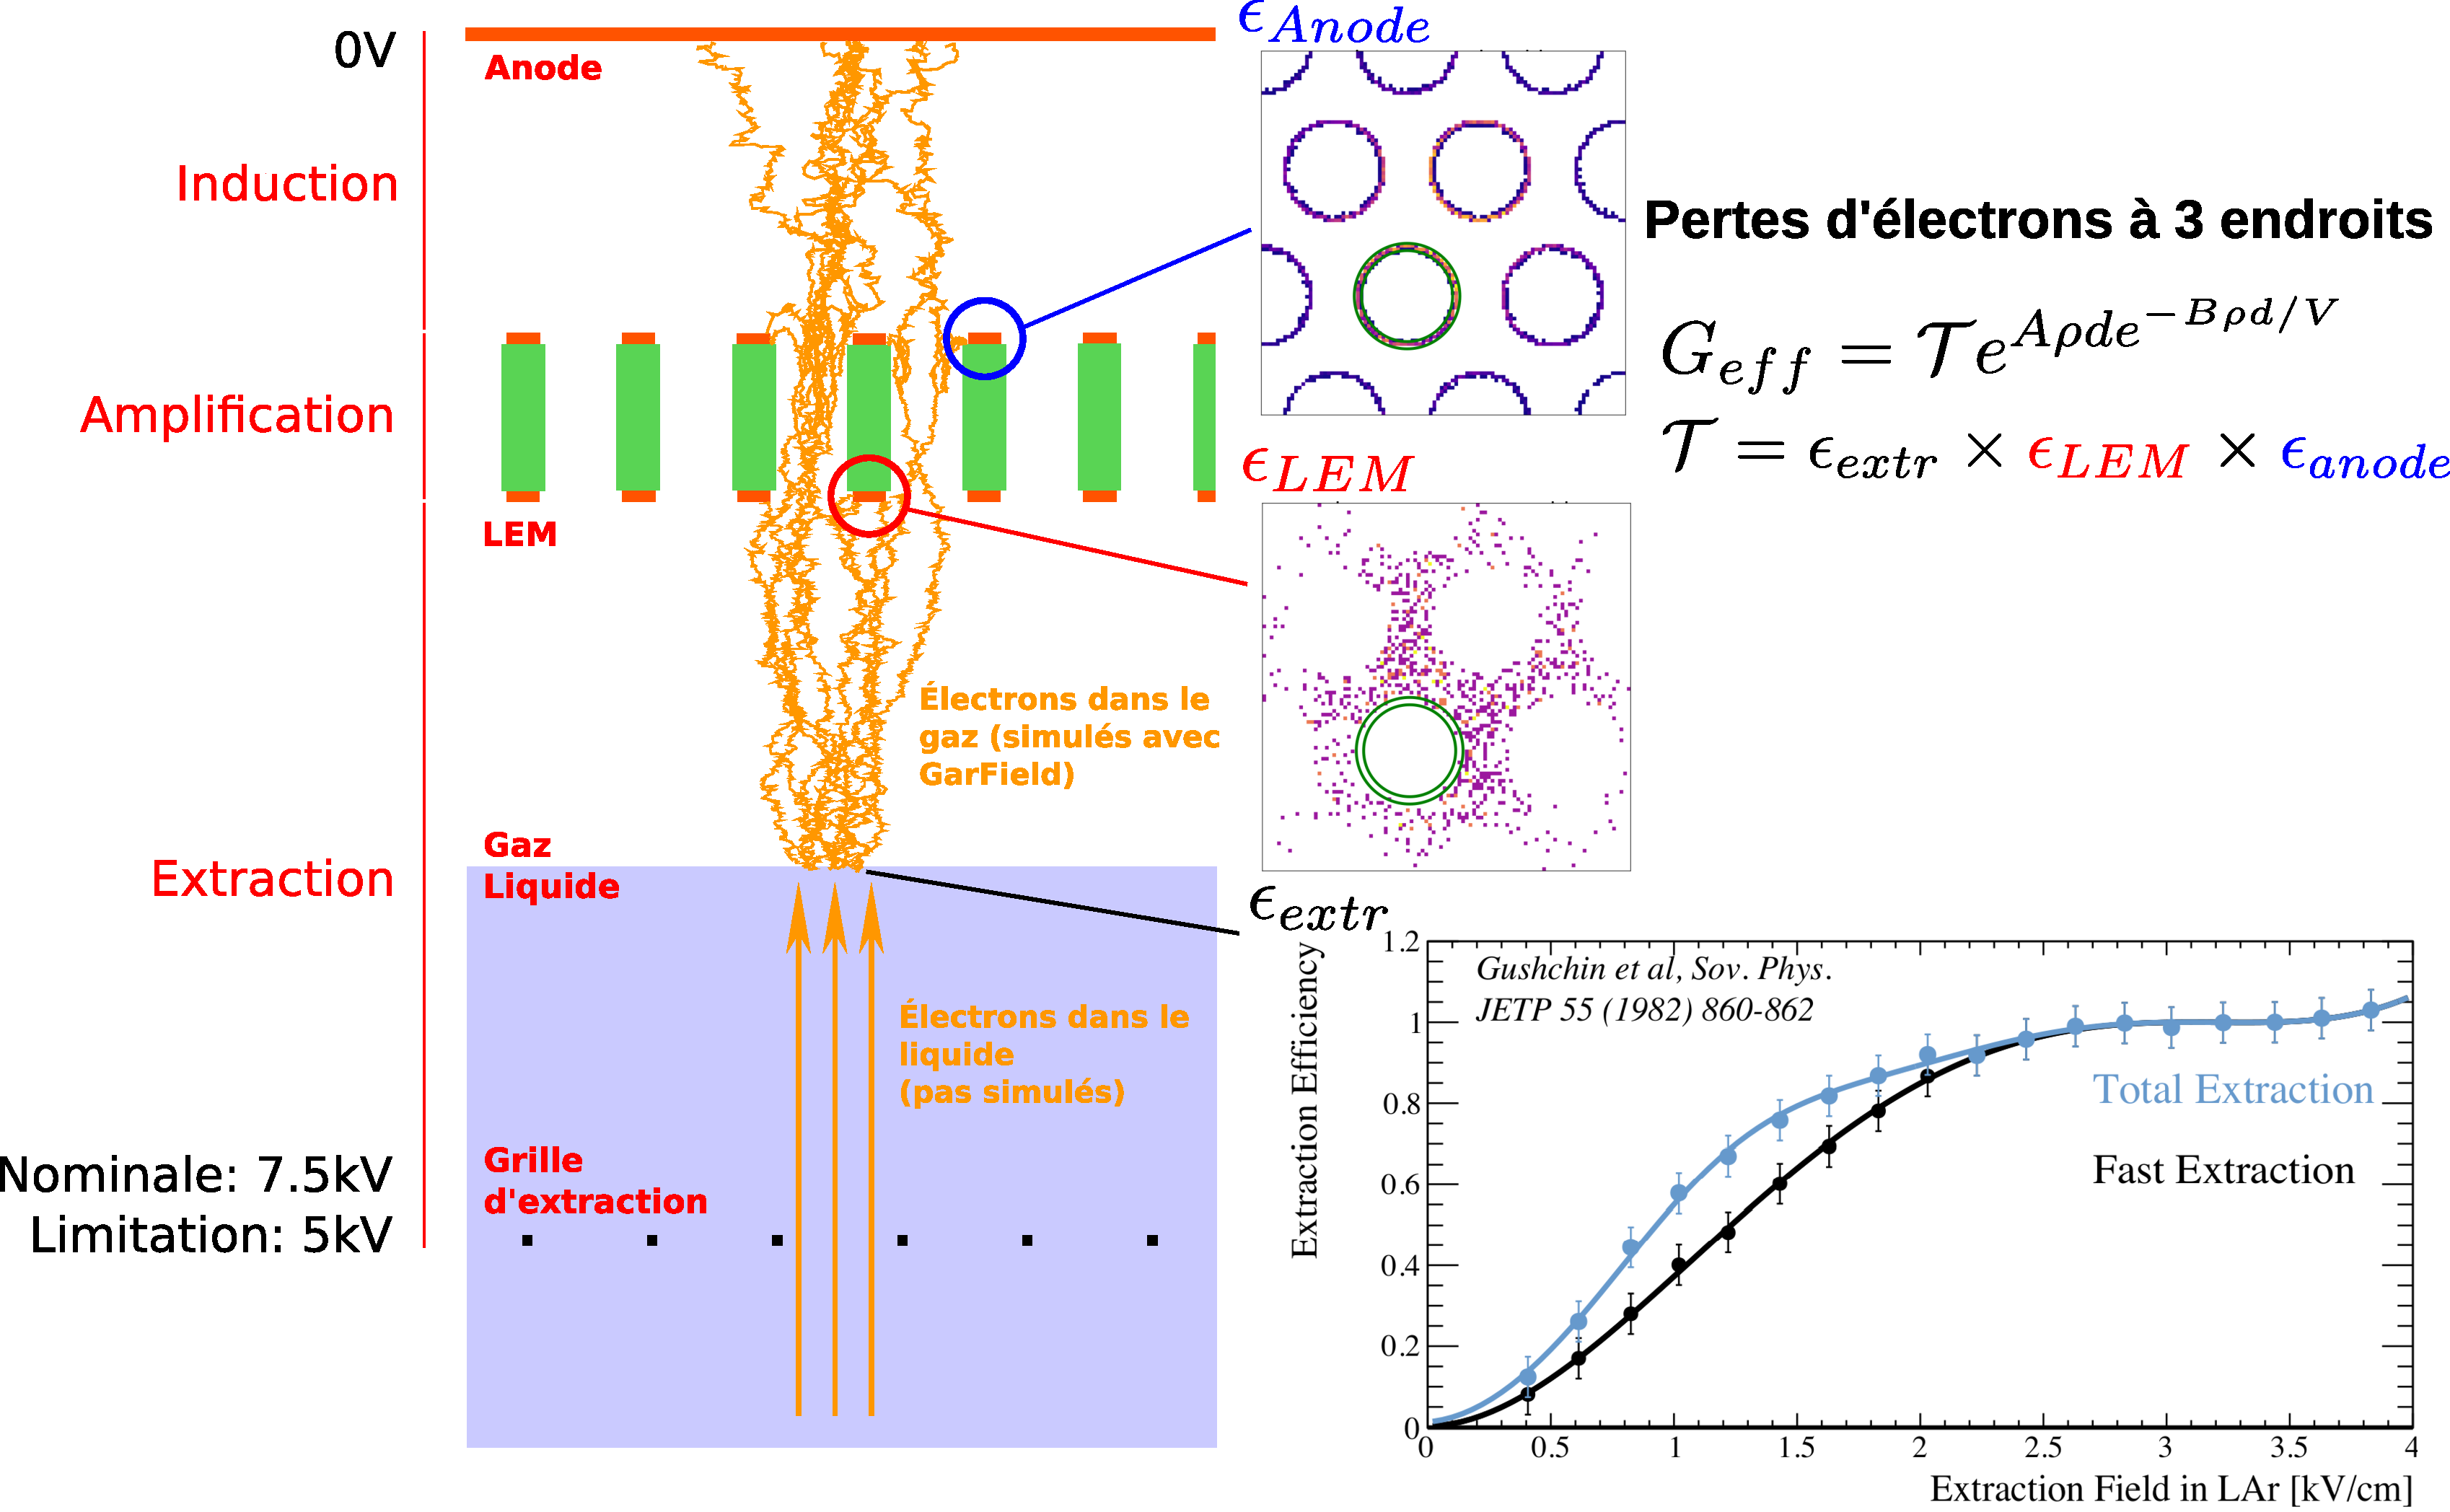
\includegraphics[width=\textwidth]{./pictures/coll_proba_2.pdf}
    \end{frame}
    
    \begin{frame}{Efficacités de collection}{Outils de simulation}
        \begin{scriptsize}
            \begin{columns}
                \begin{column}{0.5\textwidth}
                    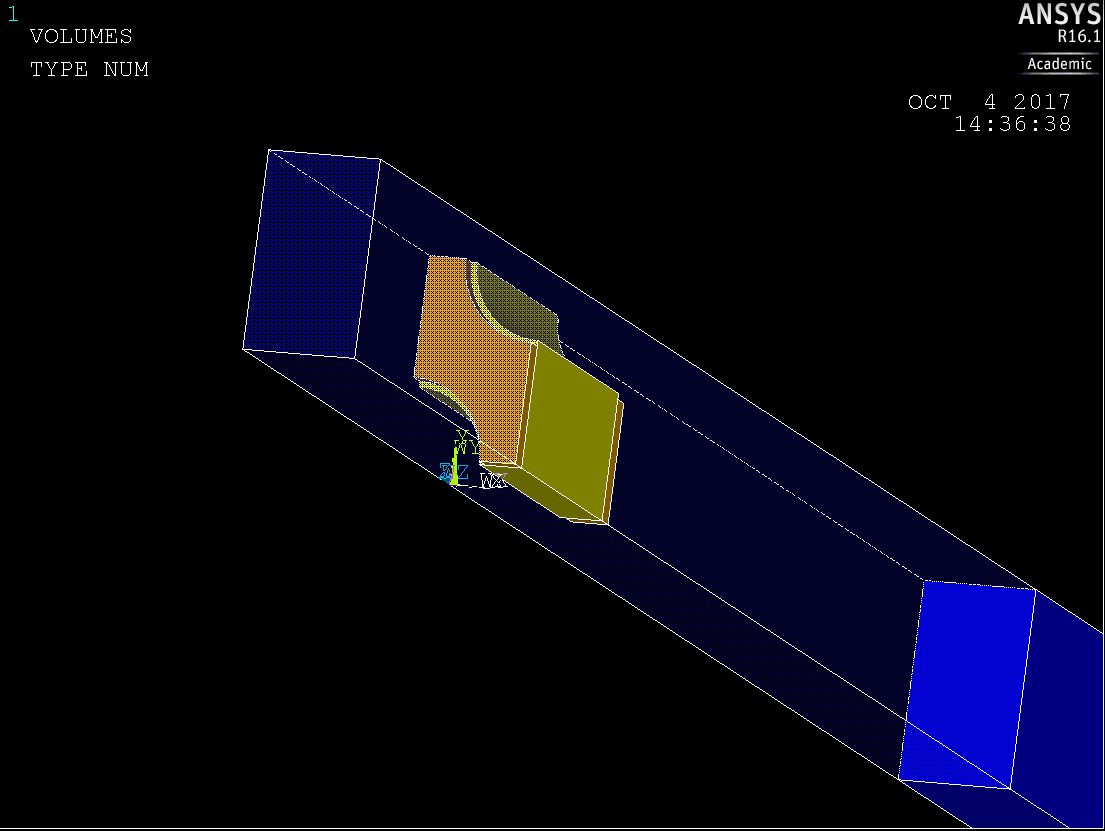
\includegraphics[width=\textwidth]{ansys_geom.png}
                \end{column}\hfill
                \begin{column}{0.5\textwidth}
                    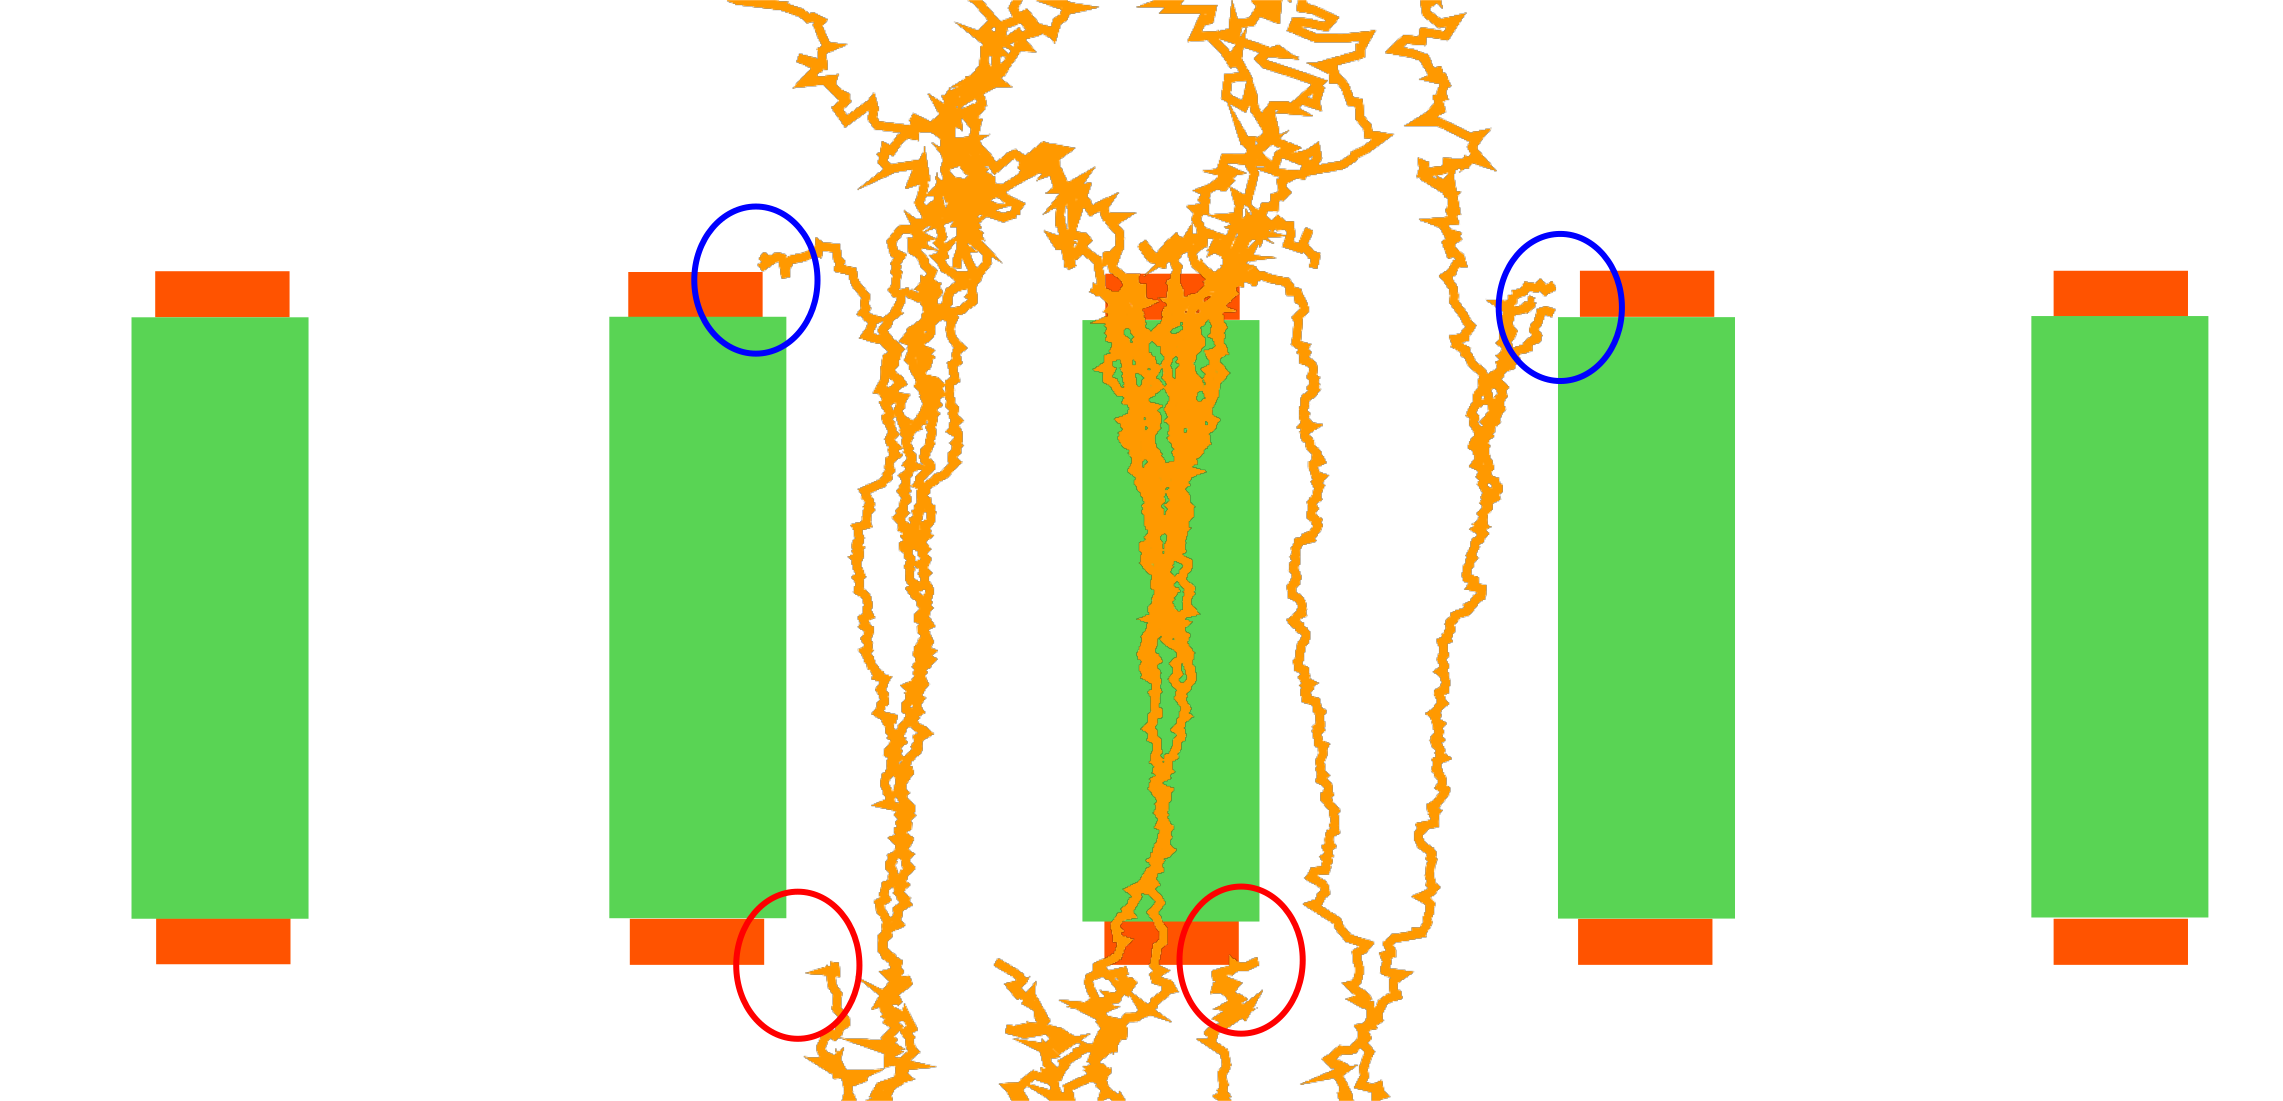
\includegraphics[width=\textwidth]{./pictures/losses_with_lem.png}
                \end{column}
            \end{columns}
            \begin{columns}
                \begin{column}{0.5\textwidth}
                    \begin{itemize}
                        \item Champ à travers le CRP simulé avec ANSYS (éléments finis)
                        \item Définit un élément de base de la géométrie en nid d'abeille, conditions de symétrie pour générer toute la géométrie
                    \end{itemize}
                \end{column}
                \begin{column}{0.5\textwidth}
                    \begin{itemize}
                        \item Cartes de champs intégrées dans GarField : simulation de dérive des électrons à travers le CRP
                        \item Capable de retracer le parcours microscopique des électrons dans l'argon gazeux
                    \end{itemize}
                \end{column}
            \end{columns}
        \end{scriptsize}
    \end{frame}
    

    \begin{frame}{Efficacités de collection}{Résultats}
        \hbox{
        		$\mathbf{G_{eff}=G_{LEM}\boldsymbol{\times}\boldsymbol{\epsilon}_{extr} \boldsymbol{\times}\textcolor{red}{\epsilon_{LEM}}\boldsymbol{\times} \textcolor{blue}{\epsilon_{anode}}}$
        	}\vspace{0.2cm}
      		\begin{columns}
            \begin{column}{0.5\textwidth}
                \centering $\textcolor{red}{\epsilon_{LEM}}$
                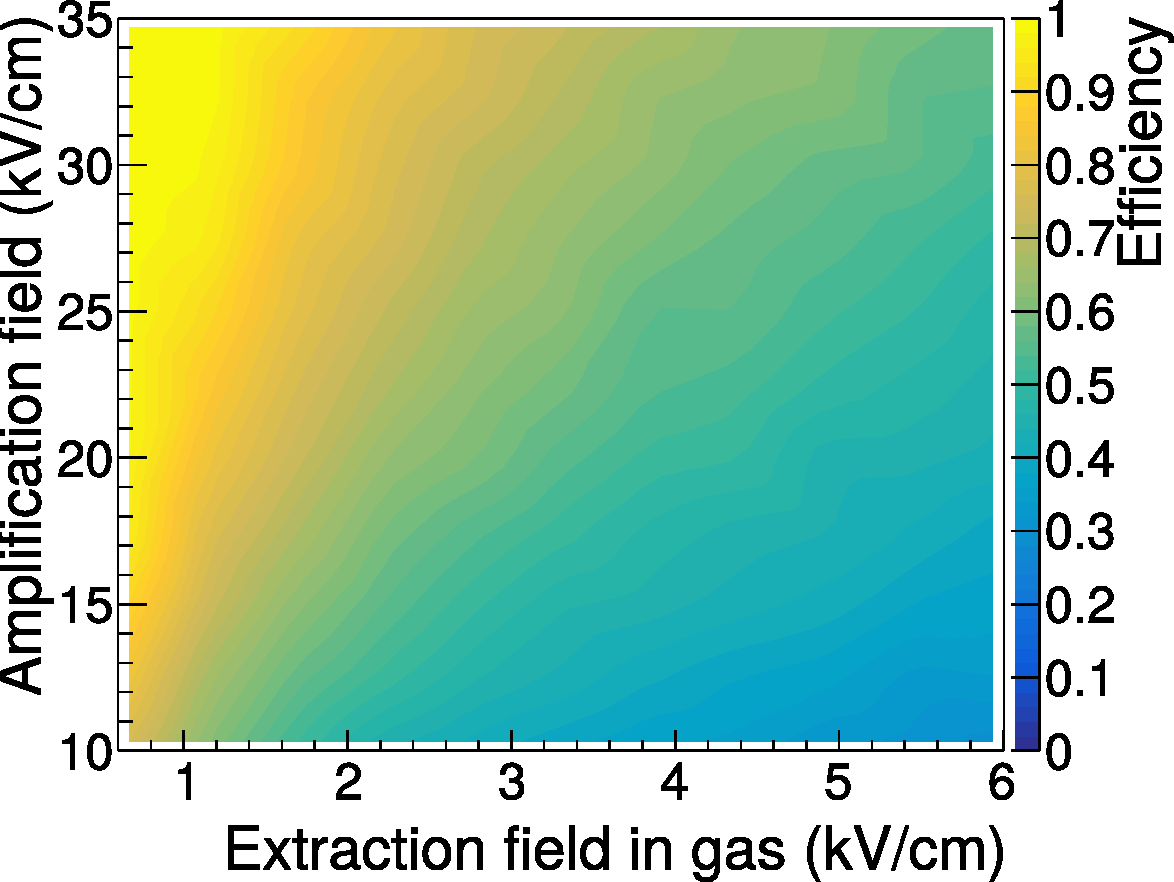
\includegraphics[width=\textwidth]{./pictures/eff_lem_alone.pdf}
            \end{column}\hfill
            \begin{column}{0.5\textwidth}
                \centering $\textcolor{blue}{\epsilon_{Anode}}$
                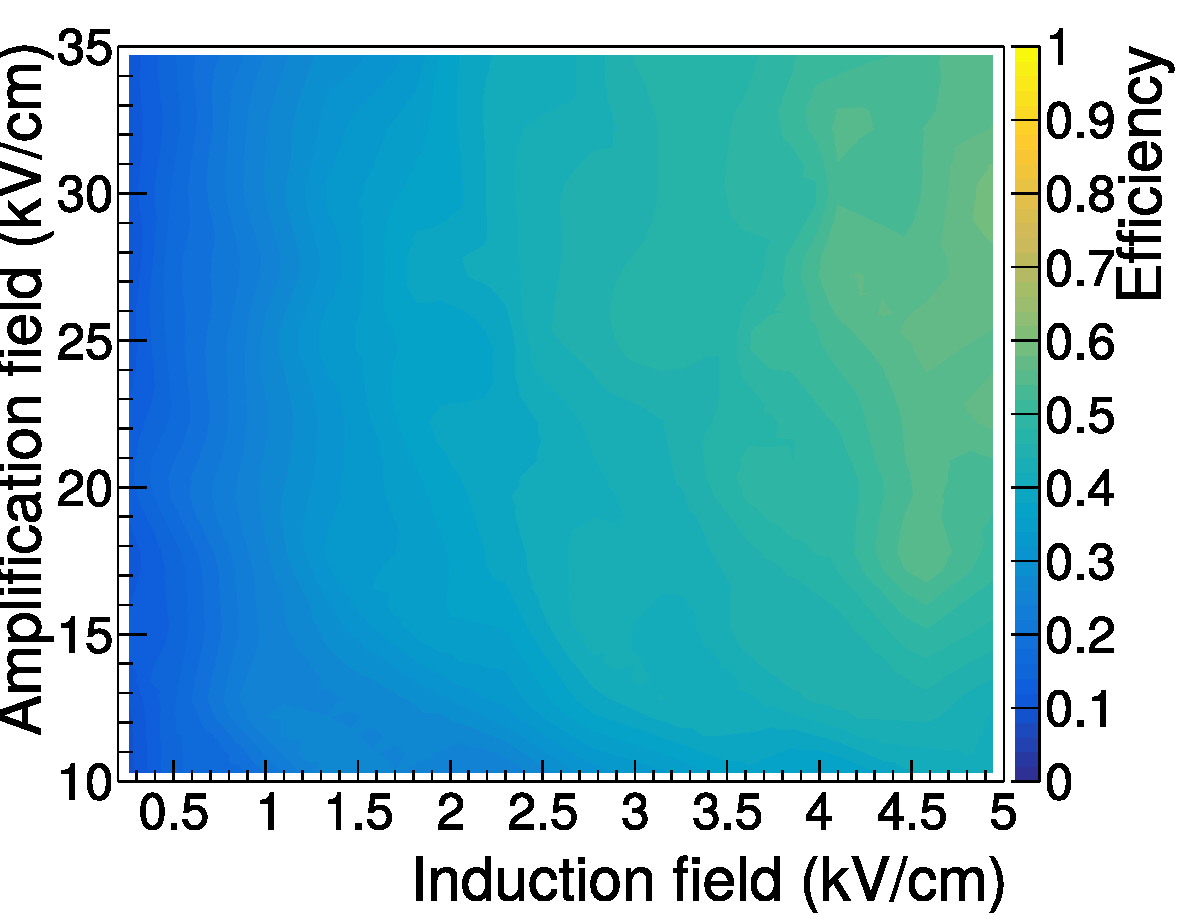
\includegraphics[width=\textwidth]{eff_anode.pdf}
            \end{column}
        \end{columns}
      		\begin{columns}
            \begin{column}{0.5\textwidth}
                \begin{scriptsize}
                    \begin{itemize}
                        \item Dépend du champ dans le gaz entre l'interface et le LEM
                        \item Champ calculable à partir de la tension grille--LEM et de la position de l'interface
                    \end{itemize}
                \end{scriptsize}
            \end{column}\hfill
            \begin{column}{0.5\textwidth}
              \begin{scriptsize}
                \begin{itemize}
                    \item Dépend du charging up du LEM
                    \item Simulée ici avant charging up
                \end{itemize}
              \end{scriptsize}
            \end{column}
        \end{columns}
    \end{frame}
    
    \begin{frame}{Efficacités de collection}{Mesures à Saclay : argon gazeux, \SI{3.3}{\bar}, source $^{241}$Am}
        $\mathbf{G_{eff}=G_{LEM}\boldsymbol{\times}\boldsymbol{\epsilon}_{extr} \boldsymbol{\times}\textcolor{red}{\epsilon_{LEM}}\boldsymbol{\times} \textcolor{blue}{\epsilon_{anode}}}$\\\vspace{0.2cm}
        
        \begin{scriptsize}
         Mesure de $G$ vs $E_{extr}$ et $E_{ind}$, puis normalisation aux efficacités simulées.\\\vfill
        \begin{columns}
            \begin{column}{0.5\textwidth}
                \centering $\textcolor{red}{\epsilon_{LEM}}$
                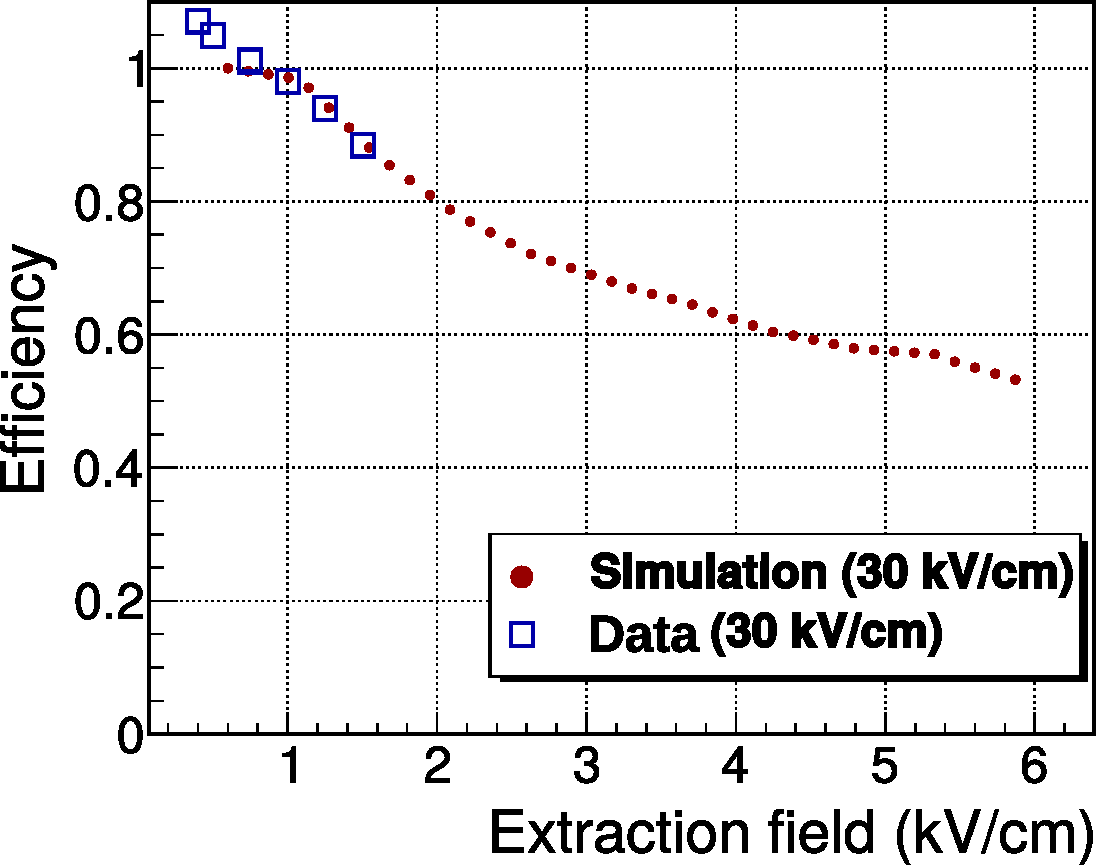
\includegraphics[width=\textwidth]{./pictures/eff_lem_gamelle.pdf}
            \end{column}\hfill
            \begin{column}{0.5\textwidth}
                \centering $\textcolor{blue}{\epsilon_{Anode}}$
                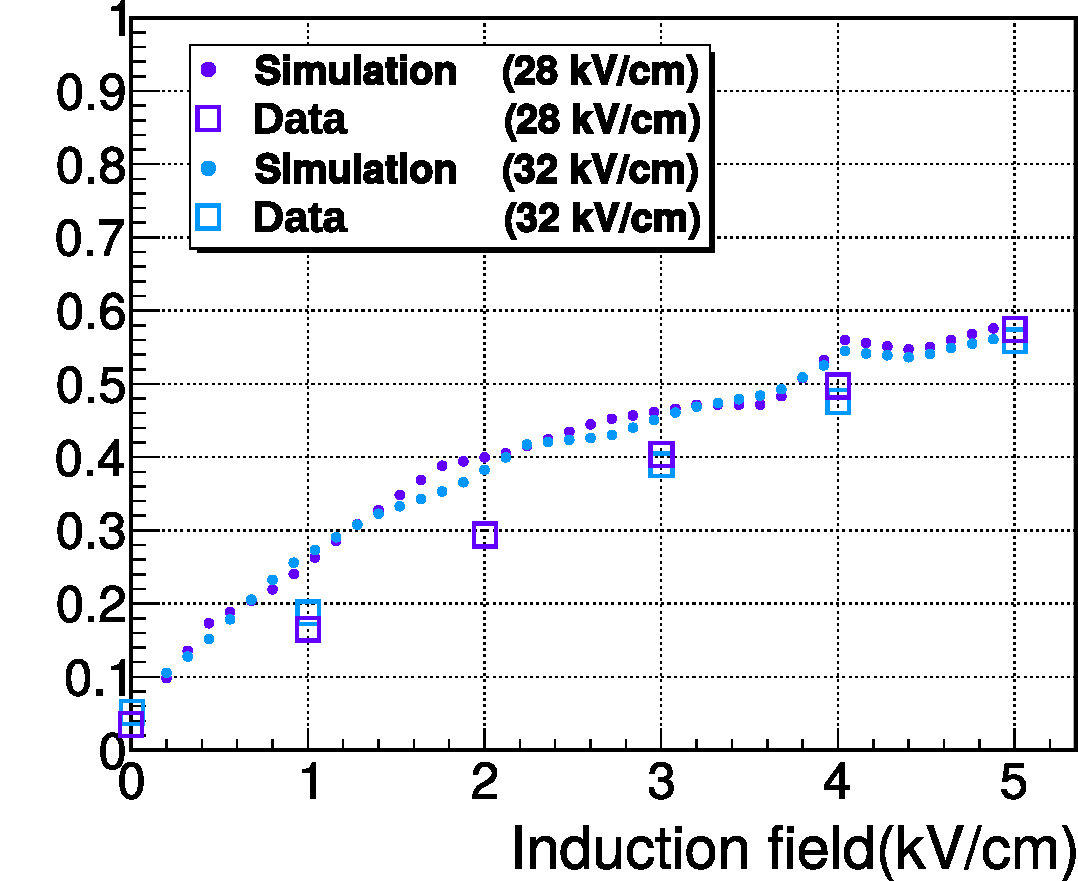
\includegraphics[width=\textwidth]{./pictures/eff_anode_gamelle.pdf}
            \end{column}
        \end{columns}
      		\begin{columns}
            \begin{column}{0.5\textwidth}
                \begin{itemize}
%                    \item Pas d'efficacité d'extraction (pas de liquide)
%                    \item Champ maximum limité par la distance Cathode-LEM et l'alimentation HT
                    \item Comportement similaire entre \SI{1}{\kilo\volt\per\centi\meter} et \SI{1.5}{\kilo\volt\per\centi\meter}
                \end{itemize}
            \end{column}\hfill
            \begin{column}{0.5\textwidth}
                \begin{itemize}
                    \item Comportement similaire, mais différences allant jusqu'à 15\,\%
                    \item[\textcolor{red}{\danger}] Mesures faites après charging up, simulations faites avant charging up!
                \end{itemize}
            \end{column}
        \end{columns}
        \end{scriptsize}
    \end{frame}

    \begin{frame}{Efficacités de collection}{Mesures dans le \TOO{}}
        \begin{scriptsize}
            \centering
            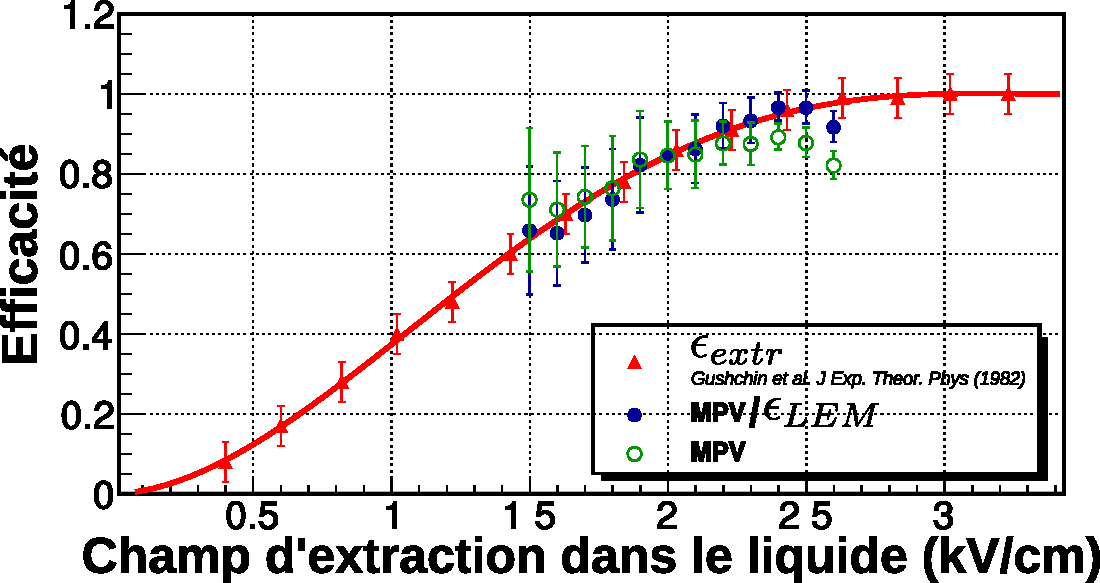
\includegraphics[width=0.75\textwidth]{./pictures/comp_311_eff.pdf}
            \vspace{0.2cm}
            \begin{columns}
                \begin{column}{0.5\textwidth}
                    \begin{itemize}
                        \item Champs d'amplification (\SI{28}{\kilo\volt\per\centi\meter}) et d'induction (\SI{1}{\kilo\volt\per\centi\meter}) constants
                        \item Grandes barres d'erreur à faibles champs dues aux imperfections de la planéité
                    \end{itemize}
                \end{column}
                \begin{column}{0.5\textwidth}
                    \begin{itemize}
                        \item MPV Normalisée à $\epsilon_{extr}$ à \SI{2}{\kilo\volt\per\centi\meter} pour comparer le comportement
                        \item La MPV divisée par  $\epsilon_{LEM}$ est meilleure que la MPV seule.
                    \end{itemize}
                \end{column}
            \end{columns}
            \vfill
            \textbf{Note :} Erreurs = systématiques, corrélées d'un point à l'autre
        \end{scriptsize}
    \end{frame}

    \begin{frame}{Efficacités de collection}{Impact sur la précision du gain}
        \begin{center} \vspace{-0.5cm}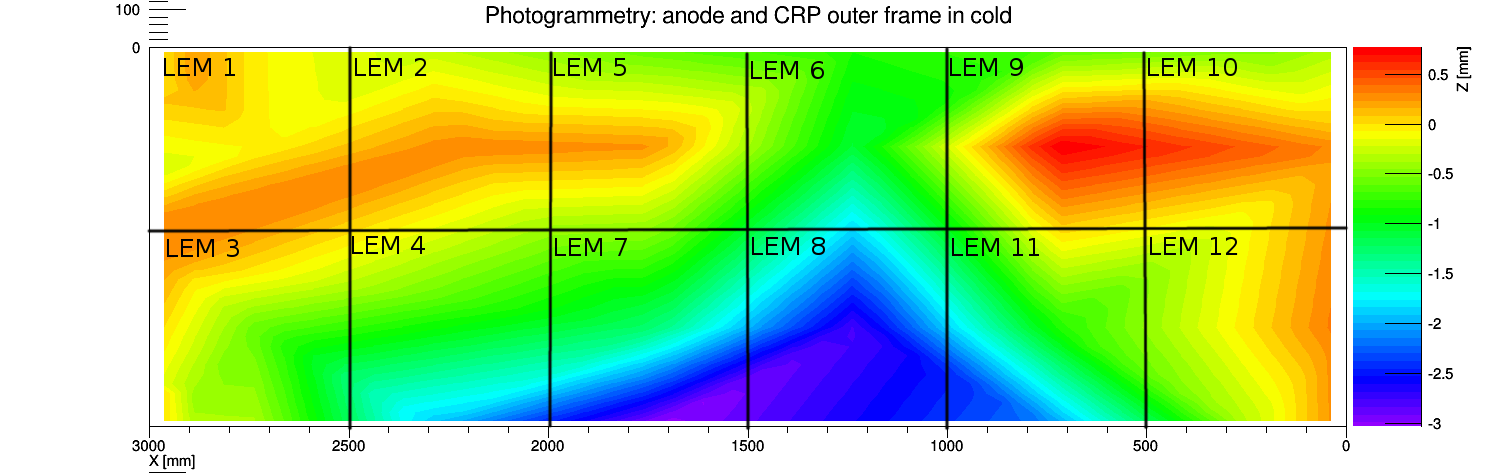
\includegraphics[width=\textwidth]{CRP-metrologie.png} \end{center}
        \begin{scriptsize}
            \begin{columns}
                \begin{column}{0.6\textwidth}
                    \centering 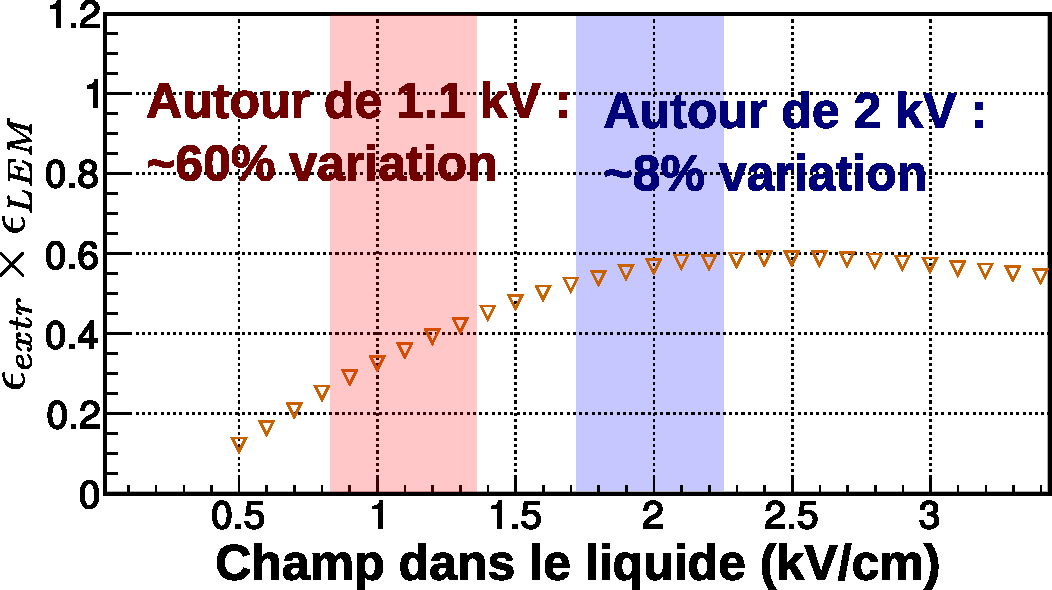
\includegraphics[width=\textwidth]{./pictures/extr_eff.pdf}
                \end{column}\hfill
                \begin{column}{0.4\textwidth}
                    \begin{itemize}
          					\item Déformation du CRP : $\pm\SI{1.8}{\milli\meter}$
          					\item[$\Rightarrow$]  25\,\% variation des champs entre la grille et l'interface et entre l'interface et les LEMs
          					\item Variation de $\epsilon_{extr}\times\epsilon_{LEM}$ à basse tension d'extraction
          				\end{itemize}
                     \textbf{Note : } dans le \SSS{},  $\Delta V$~Grille-LEM $\sim\SI{3}{\kilo\volt}$\\
                     $\Rightarrow$ efficacité $\sim$ constante.
                \end{column}
            \end{columns}
        \end{scriptsize}
    \end{frame}

    \begin{frame}{Stabilité du gain à travers le CRP dans le \TOO{}}
        \begin{scriptsize}
            \centering Deux acquisitions à 12 heures d'intervalle.\\
            Extraction \SI{1.9}{\kilo\volt\per\centi\meter}, Amplification \SI{28}{\kilo\volt\per\centi\meter}, Induction \SI{1.5}{\kilo\volt\per\centi\meter}\\\vspace{0.2cm}
            \begin{center} \vspace{-0.5cm}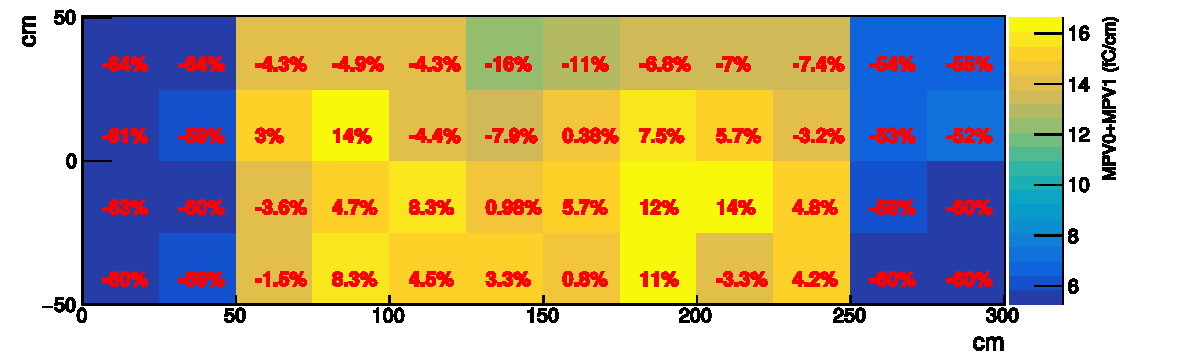
\includegraphics[width=0.9\textwidth]{dQds_2D_840.pdf} \end{center}
            \begin{center} \vspace{-0.5cm}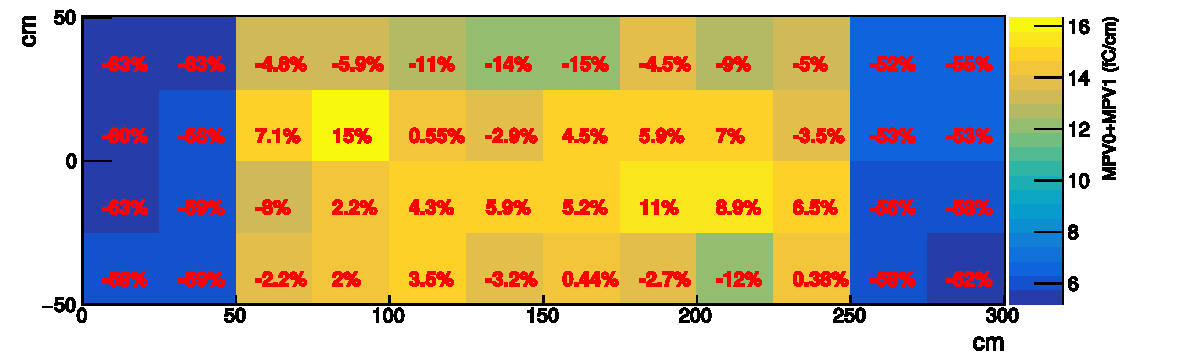
\includegraphics[width=0.9\textwidth]{dQds_2D_842.pdf} \end{center}
            \vspace{-0.5cm}
            \begin{itemize}
       			\item Variations attendues : $\pm 12 \,\%$ (épaisseur des LEMs et planéité du CRP)
       			\item Variations observées jusqu'à $\sim \pm15\,\%$
   			\end{itemize}
        \end{scriptsize}
    \end{frame}

  \subsection{Zones mortes}
    
    \begin{frame}{Zones mortes}{Simulations}
       	\begin{scriptsize}
       		\begin{minipage}{0.38\textwidth}
       			\begin{center}
       				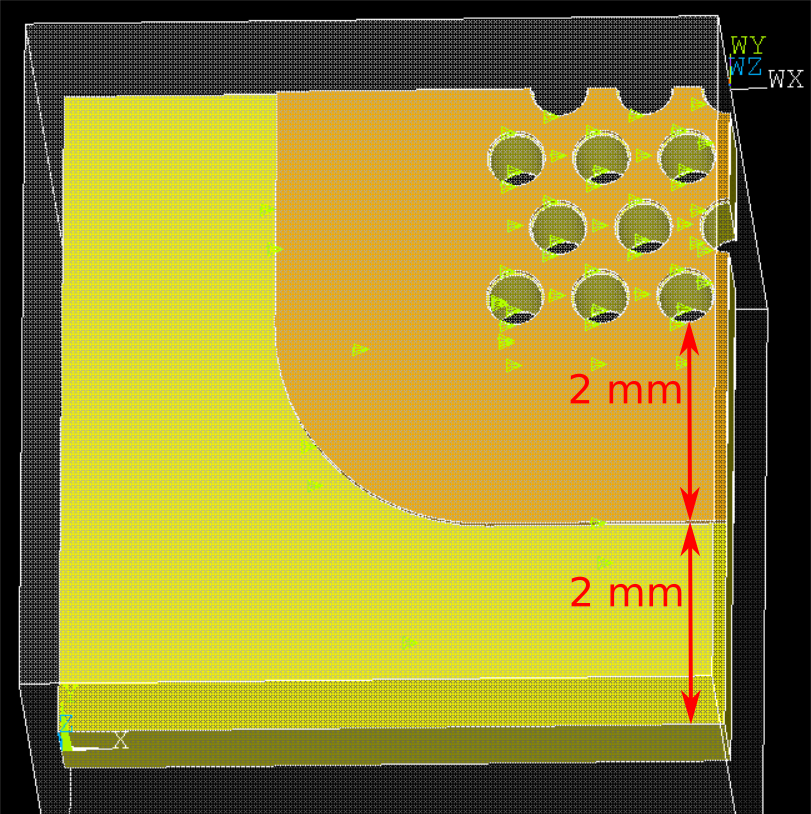
\includegraphics[width=0.8\textwidth]{corner_annotations.png}\\
       				design : CFR-34\\
       			\end{center} 
       			Zones mortes = zones sans trous d'amplification:
       			\begin{itemize}
       				\item Bords du LEM
       				\item Trous des vis.
       				\item Connecteurs haute tension.
       			\end{itemize}
       			$\Rightarrow$ Pertes de charges\\
       			$\Rightarrow$ Dégrade la résolution en énergie\\
       		\end{minipage}
       		\begin{minipage}{0.58\textwidth}
       			\centering
       			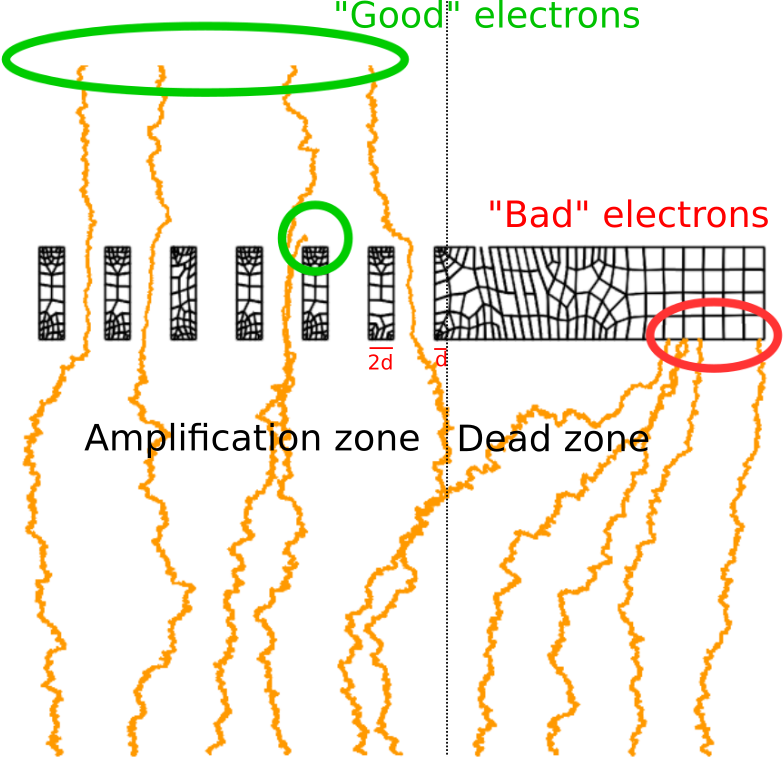
\includegraphics[width=0.8\textwidth]{drift_example.png}\\
       			\vspace{0.5cm} \hspace{0.1cm}
       			\begin{minipage}{0.48\textwidth}
       				\centering
       				\textbf{Carte d'efficacité}\\
       				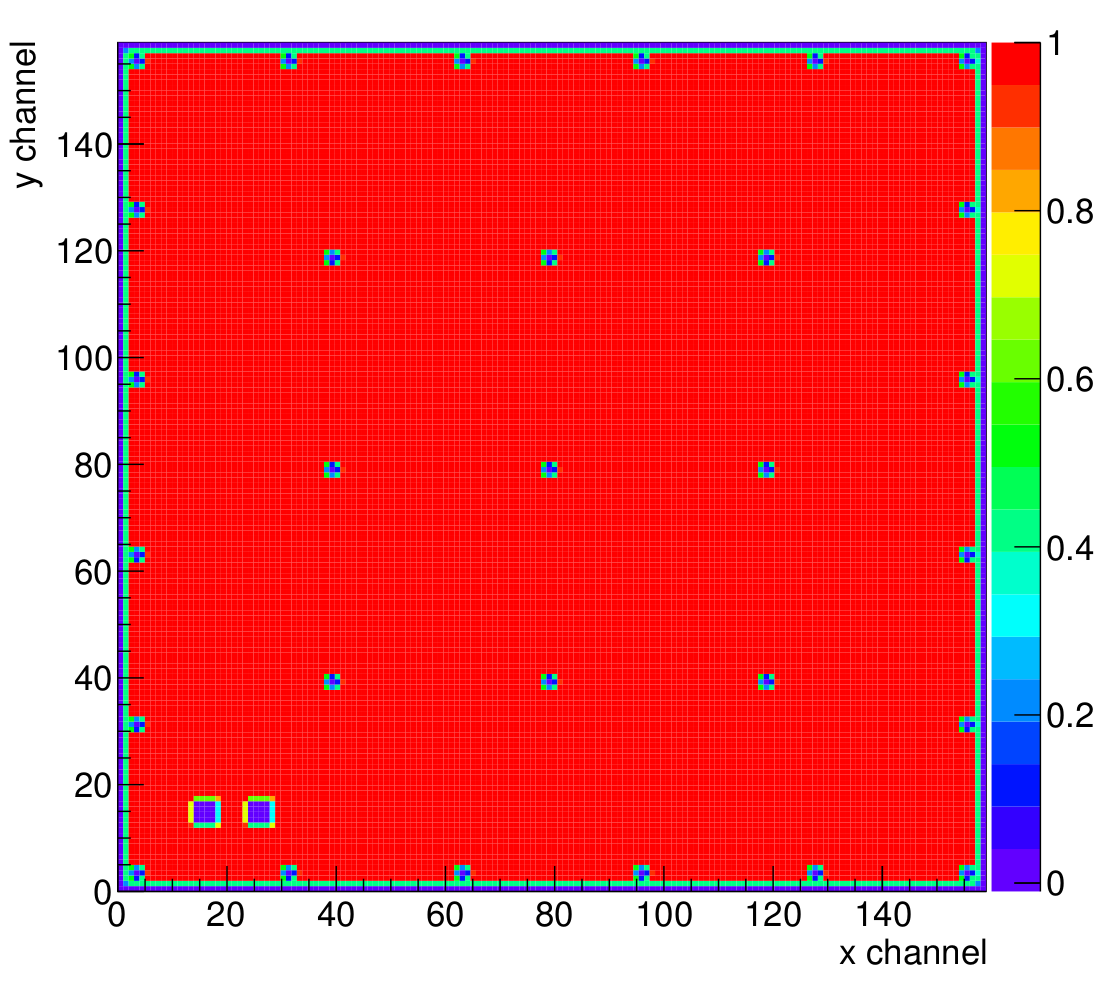
\includegraphics[width=\textwidth]{eff_map.png}
       			\end{minipage}\hfill
       			\begin{minipage}{0.48\textwidth}
       				\centering
       				\textbf{Charge collectée d'électrons de \SI{3}{\giga\eV}}\\
       				\includegraphics[width=1.2\textwidth]{./pictures/electron.png}
       			\end{minipage}
       		\end{minipage}
       	\end{scriptsize} 
    \end{frame}

    \begin{frame}{Zones mortes dans le \TOO{}}{MPV mesurée sur les bords des LEMs}
        \begin{scriptsize}
            \centering \textbf{Charge déposée sur les bords des anodes (12 canaux parmi 1280)}
            \begin{columns}
                \begin{column}{0.5\textwidth}
                    \includegraphics[width=\textwidth]{./pictures/dQds_840_0_border.pdf}
                \end{column}
                \begin{column}{0.5\textwidth}
                    \includegraphics[width=\textwidth]{./pictures/dQds_840_1_border.pdf}
                \end{column}
            \end{columns}
            \begin{columns}
                \begin{column}{0.5\textwidth}
                    \begin{itemize}
                        \item 35\,\% inférieure à la MPV mesurée sur les autres canaux.
                        \item Prédiction des simulations : 60\,\% de pertes
                    \end{itemize}
                \end{column}
                \begin{column}{0.5\textwidth}
                    \begin{itemize}
                        \item Simulation faite aux champs nominaux
                        \item Mesures faites à plus bas champs
                        \item[$\Rightarrow$] Champs électriques différents, peut expliquer la différence 
                    \end{itemize}
                \end{column}
            \end{columns}
        \end{scriptsize}
    \end{frame}

    \subsection{Charging up}
    \begin{frame}{Charging up dans le \TOO{}}
        \begin{scriptsize}
            \includegraphics[width=\textwidth]{charging_up.pdf}
            \begin{itemize}
                \item Charging up $\sim$ linéaire
                \item Pris en compte dans la mesure du gain effectif
                \item Persiste une fois la tension coupée
            \end{itemize}
        \end{scriptsize}
    \end{frame}
    
  \subsection{Gain vs champ d'ampli.}

    \begin{frame}{Gain effectif vs champ d'amplification}{Extrapolation aux conditions du \SI{3}{\liter}}
        \begin{scriptsize}
            \centering \includegraphics[width=\textwidth]{./pictures/gain_vs_ampli.pdf} \\
%            \vspace{0.2cm}
%            \begin{columns}
%                \begin{column}{0.5\textwidth} 
%                    \begin{itemize}
%                        \item  \textcolor{red}{Bon accord avec le \threeL{} après charging up}
%                        \item[$\Rightarrow$] Charging up complet.
%                    \end{itemize}
%                \end{column}
%                \begin{column}{0.5\textwidth}
%                    Petite différence avec \SI{3}{\liter} :
%                    \begin{itemize}
%                        \item Différences d'épaisseur? 
%                        \item $\textcolor{blue}{\epsilon_{Anode}}$?
%                    \end{itemize}
%                \end{column}
%            \end{columns}
        \end{scriptsize}
    \end{frame}
    
    \begin{frame}{Gain effectif vs champ d'amplification}{Extrapolation aux conditions du \SI{3}{\liter}}
        \begin{scriptsize}
            \centering \includegraphics[width=\textwidth]{./pictures/gain_vs_ampli_circle.pdf} \\ 
%            \begin{columns}
%                \begin{column}{0.5\textwidth}
%                    \textcolor{red}{Run au delà de \SI{28}{\kilo\volt\per\centi\meter}} : très grandes barres  d'erreurs 
%                    \begin{itemize}
%                        \item  Plus grand champ d'ampli $\Rightarrow$ plus grand impact des variations d'épaisseurs des LEMs
%                         \item Plus faible champ d'extraction ($\sim \SI{1}{\kilo\volt\per\centi\meter}$) $\Rightarrow$ plus grand impact des imperfections de planéité
%                    \end{itemize}
%                \end{column}
%                \begin{column}{0.5\textwidth}
%                    \begin{itemize}
%                        \item Faible champ d'extraction $\Rightarrow$ étalement en temps du signal.
%                        \item[$\Rightarrow$] Difficultés de reconstruction
%                        \item Développement d'un algorithme de reconstruction dédié
%                    \end{itemize}
%                \end{column}
%            \end{columns}
        \end{scriptsize}
    \end{frame}
     
    \begin{frame}{Gain effectif vs champ d'amplification}{Extrapolation aux conditions du \SI{3}{\liter}}
        \begin{Large}
            {\transparent{0.4}\centering\vspace{0.42cm}\includegraphics[width=\textwidth]{gain_vs_ampli_circle.pdf}}
            \begin{textblock*}{\textwidth}(2cm,0.6\textheight)
                \centering \textbf{Reconstruction des traces à bas champ d'extraction}
            \end{textblock*}
        \end{Large}
    \end{frame}
    
    \begin{frame}{Problème lors de la suppression du bruit cohérent}
        \begin{scriptsize}
            \begin{columns}
                \begin{column}{0.45\textwidth}
                    \centering \textbf{Signal trouvé:}\\
                    \centering \includegraphics[width=\textwidth]{./pictures/good_pedsub.png}\\
                    \centering \includegraphics[width=\textwidth]{./pictures/good_cnsub.png}\\
                    \centering \textbf{Signal non trouvé:}\\
                    \centering \includegraphics[width=\textwidth]{./pictures/pedsub_adcs_high_threshold.pdf}\\
                    \centering \includegraphics[width=\textwidth]{./pictures/cnsub_adcs_high_threshold.pdf}\\
                 \end{column}
                \begin{column}{0.55\textwidth}
                    \textbf{Bruit cohérent = bruit commun à tous les canaux d'une même carte d'électronique.} \\\vspace{0.3cm}
                    Suppression du bruit cohérent :
                    \begin{itemize}
                        \item regroupement des canaux par groupe de 32
                        \item Calcul de la moyenne d'ADC pour chaque bin de temps
                        \item Soustraction de cette moyenne par bin de temps dans chaque canal d'ADC
                    \end{itemize} 
                    \vspace{0.3cm}
                    \textbf{ Exemple d'un canal d'ADC avant et après suppression du bruit cohérent dans le run à \SI{30}{\kilo\volt\per\centi\meter} }: \\Le coup n'est pas vu et n'est pas ignoré pour le calcul du bruit cohérent.  Suppression trop forte \\
                    $\Rightarrow$ coup supprimé \\
                    $\Rightarrow$ Trace segmentée \\
                    $\Rightarrow$ Mauvaise reconstruction avec LArSoft \\
                \end{column}
            \end{columns}
        \end{scriptsize}
    \end{frame}

    \begin{frame}{Reconstruction avec LArSoft}
        \begin{scriptsize}
            \begin{columns}
                \begin{column}{0.65\textwidth}
                    \centering \textbf{Exemple de reconstruction, haute extraction}\\
                    \centering \includegraphics[width=\textwidth]{event_larsoft.png}
                \end{column}
                \begin{column}{0.35\textwidth}
                    \centering \textbf{Exemple de distribution $dQ/ds$, basse extraction}\\
                    \centering \includegraphics[width=\textwidth]{dQds_1197_0.pdf}
                \end{column}
            \end{columns}\vfill
            \begin{columns}
                \begin{column}{0.5\textwidth}
                    \textbf{Reconstruction avec LArSoft :}
                    \begin{enumerate}
                        \item Identification des régions de signal
                        \item Nombreux passages de suppression de bruit
                        \item Identification des coups dans chaque vue, regroupement en amas 2D, calcul de $dQ$
                        \item Identification des amas 3D et calcul de $ds$
                    \end{enumerate}
                \end{column}
                \begin{column}{0.5\textwidth}
                    Coups sont ignorés $\Rightarrow$ trace segmentée\\
                    $\Rightarrow$ Mauvaise identifications des amas 3D et mauvais calcul de $ds$
                \end{column}
            \end{columns}
        \end{scriptsize}
    \end{frame}
    
    \begin{frame}{Solution : transformation de Hough}
        \textbf{Paramétrisation d'une droite }: $r=x\cos(\theta)+y\sin(\theta)$\\
        \textbf{Calcul de $\boldsymbol{r}$ pour $\boldsymbol{\theta\in[0,\pi]}$} : un point dans un repère cartésien correspond à une sinusoïde dans l'espace de Hough\\
        $\Rightarrow$ Un ensemble de points sur une même droite dans un repère cartésien correspond à un point dans l'espace de Hough\\
        $\Rightarrow$ \textcolor{red}{Trouver une droite revient à trouver un maximum local}\\\vfill
        \includegraphics[width=\textwidth]{./pictures/HT.pdf}
    \end{frame}

    \begin{frame}{Reconstruction avec la transformation de Hough}
        \begin{scriptsize}
            \begin{columns}
                \begin{column}{0.5\textwidth}
                    \textbf{Nouvelle méthode de reconstruction :}
                    \begin{enumerate}
                        \item Identification des régions de signal
                        \item Un passage de suppression de bruit cohérent
                        \item Identification des coups
                        \item \textbf{Transformation de Hough} : \textcolor{red}{cherche des droites et non des segments}
                        \item \textbf{Seconde suppression du bruit sachant où sont les traces}, calcul de $dQ/ds$
                    \end{enumerate}
                    $\Rightarrow$ Une trace segmentée peut être reconstruite comme une droite
                \end{column}
                \begin{column}{0.5\textwidth}
                    \centering \includegraphics[width=0.8\textwidth]{HT_real_data.pdf}
                \end{column}
            \end{columns}
            \begin{center} \includegraphics[width=0.8\textwidth]{HT_real_data_track.pdf} \end{center}
        \end{scriptsize}
    \end{frame}

    \begin{frame}{Reconstruction avec la transformation de Hough}
        \begin{scriptsize}
            \begin{center} \includegraphics[width=0.8\textwidth]{./pictures/cnsub_fromtrack.pdf} \end{center}
            \begin{columns}
                \begin{column}{0.6\textwidth}
                    \centering Transformation de Hough\\
                    \includegraphics[width=0.95\textwidth]{1197_dQds_0.pdf}
                \end{column}
                \begin{column}{0.4\textwidth}
                    \centering LArSoft\\
                    \includegraphics[width=\textwidth]{dQds_1197_0.pdf}
                \end{column}
            \end{columns}
        \end{scriptsize}
    \end{frame}
    
    \begin{frame}{Gain effectif vs champ d'amplification}
        \begin{scriptsize}
            \centering \includegraphics[width=\textwidth]{./pictures/gain_vs_ampli_full.pdf} \\ 
        \end{scriptsize}
    \end{frame}
    
    \begin{frame}{Résultats du \TOO{}}
        \begin{itemize}
           	\item Fonctionnement d'une DLArTPC de \SI{4}{\tonne} : \textcolor{green}{\checkmark}
            \item Gain vs champ d'amplification en bon accord avec les résultats précédents : \textcolor{green}{\checkmark}
         	\item Impuretés $<\SI{75}{ppt}$ equiv. $O_2$ : \textcolor{green}{\checkmark} (but $<\SI{100}{ppt}$)
         	\item Scintillation clairement détectée --  utilisée comme déclencheur et $t_0$: \textcolor{green}{\checkmark}
%           	\item Signal/Bruit : $\sim$ 10 pour une MIP
       	\end{itemize}
   	\end{frame}
    
    \section[\SSS{}]{Tests et métrologie des détecteurs gazeux de type MPGD (LEMs) du démonstrateur de \SSS{}}

    {
    	\usebackgroundtemplate{\includegraphics[width=\paperwidth]{./pictures/1.pdf}}
        \begin{specialframe}
            \vspace{2cm}\hspace*{-1.8cm}\parbox[t]{\textwidth}{
                \begin{center}
                    \begin{huge}
                            \textcolor{pheniics_purple}{\textbf{Tests et métrologie des LEMs et anodes du démonstrateur de \SSS{}}}
                    \end{huge}
                \end{center}
            }
        \end{specialframe}
    }

    \begin{frame}{Le démonstrateur de \SSS{}}
    	\begin{scriptsize}
                \centering
    			\vspace{-0.45cm}\includegraphics[width=\textwidth]{666_full.pdf}\\
    			\vfill
    			\textbf{Nouvelle technologie -- principaux défis :}\\
    			\vfill
    			\begin{columns}
           			\begin{column}{0.36\textwidth}
           				\hspace{-0.5cm}\begin{itemize}
           					\item \textcolor{red}{But: Gain $\geq 20$} \\(S/B $\geq 200$ pour une MIP)
           					\item \textcolor{red}{Stabilité} \\ (plusieurs années)
           				\end{itemize}
           			\end{column}
           			\begin{column}{0.37\textwidth}
           				\begin{itemize}
           					\item \textcolor{red}{Impuretés: \SI{100}{ppt}} \\ equiv. $O_2$
           					\item \SI{6}{\meter} de dérive : \SI{500}{\volt\per\centi\meter} \\ (tps de dérive $\sim\SI{3.7}{\milli\second}$) \\ $\Rightarrow$ Cathode à \textcolor{red}{\SI{300}{\kilo\volt}}
           				\end{itemize}
            		\end{column}
            		\begin{column}{0.4\textwidth}
            			\hspace{-0.5cm}\begin{itemize}
           					\item[\textcolor{red}{\danger}] Effet de charge d'espace \\ (pas dans DU$\nu$E)
            			\end{itemize}
            		\end{column}
    			\end{columns}
    	\end{scriptsize} 
    \end{frame}
    
    \begin{frame}{La responsabilité de l'Irfu}
        \centering Production, test et caractérisation des LEMs et anodes de 2 des 4 CRPs.\\\vfill
    	\begin{scriptsize}
        	\begin{columns}
            	\begin{column}{0.5\textwidth}
                	\includegraphics[width=\textwidth]{./pictures/LEM.png}\\
                   	\includegraphics[width=\textwidth]{anode_carde.png}
            	\end{column}
       	        \begin{column}{0.5\textwidth}
           	        \textbf{Tenue en tension?\\
           	        Gain?\\
           	        Uniformité de l'épaisseur des LEMs?\\
           	        Continuité des pistes des anodes?\\}\vspace{0.3cm}
           	        \begin{itemize}
               	        \item Réalisation de l'infrastructure nécessaire aux tests des LEMs et anodes
               	        \item LEMs produit par ELTOS sur la base du design testé dans le prototype de \threeL{} par ETHZ (CFR-34, été 2017)
               	        \item Modification du design afin d'atteindre une meilleure tenue en tension (CFR-35, Janvier--Octobre 2018)
               	        \item Instrumentation de 2 CRPs sur 4
           	        \end{itemize}
       	        \end{column}
        	\end{columns}
   		\end{scriptsize}
    \end{frame}
    
    \begin{frame}{Test de continuité des anodes}
        \begin{scriptsize}
            \includegraphics[width=\textwidth]{anode_cards_2.pdf}
            \begin{columns}
                \begin{column}{0.65\textwidth}
                    \centering\includegraphics[width=0.75\textwidth]{anode_test_probleme.png}
                \end{column}
                \begin{column}{0.45\textwidth}
                    \begin{itemize}
                        \item Réalisation de 4 cartes de test
                        \item 72 testées
                        \item 64 sans problèmes
                        \item 6 avec 1 canal du bord endommagés (zone morte)
                        \item 2 avec 1 canal endommagé
                    \end{itemize}
                \end{column}\hfill
            \end{columns}
        \end{scriptsize}
    \end{frame}

    \begin{frame}{Préparation des LEMs}
    	\begin{scriptsize}
    		\begin{center}
		    	\includegraphics[width=\textwidth]{pretest.png}
	    	\end{center}
	    	\begin{columns}
	    		\begin{column}{0.5\textwidth}
	    			\begin{itemize}
	    				\item $>100$ LEMs produits industriellement par ELTOS (Italie)
	    				\item Cahier des charges fournit par l'Irfu
	    			\end{itemize}
	    		\end{column}\hfill
	    		\begin{column}{0.5\textwidth}
	    			\textbf{\hspace{0.3cm}Au CEA}:
	    			\begin{enumerate}
	    				\item Contrôle de l'uniformité de l'épaisseur.
	    				\item Soudure des connecteurs et collage des espaceurs.
	    				\item Nettoyage, polymérisation, séchage.
	    			\end{enumerate}
	    		\end{column}
	    	\end{columns}
	    \end{scriptsize}
	    \vspace{0.5cm}
        $\Rightarrow$ LEMs prêts pour les tests hautes tensions et mesures de gain!
    \end{frame}

    \subsection[Épaisseur]{Mesure de l'uniformité de l'épaisseur des LEMs}

     \begin{frame}{Mesure de l'uniformité de l'épaisseur des LEMs}{Méthode expérimentale}
    	\begin{scriptsize}
    		\begin{columns}
    			\begin{column}{0.5\textwidth}
    				\begin{center}
        				\begin{normalsize}
        					$G _{eff}= \mathcal{T}e^{A\rho \textcolor{red}{d} e^{-B\rho \textcolor{red}{d}/V}}$\\
        				\end{normalsize}
    				\end{center}
    				$\textcolor{red}{d}$: \textcolor{red}{épaisseur du LEM}.\\
    				$\Rightarrow$ Impact exponentiel sur le gain.\\
    				$\Rightarrow$ Nécessaire de connaître les fluctuations de cette épaisseur pour \textcolor{red}{vérifier l'uniformité du gain}.\\
    				\vfill
    				\centering \includegraphics[height=0.6\textheight]{CCI.png}\\\vfill
    			\end{column}
    			\hfill
    			\begin{column}{0.5\textwidth}
    				\begin{itemize}
    					\item Imagerie Chromatique Confocale.
    					\item Mesure l'épaisseur des 72 LEMs du \SSS{}.
    					\item Création d'un script Python pour l'analyse des résultats.
    				\end{itemize}
    				\centering \includegraphics[height=0.6\textheight]{./pictures/plate_and_bricks.png}\\
    			\end{column}
    		\end{columns}
    	\end{scriptsize}
    \end{frame}

    \begin{frame}{Mesure de l'uniformité de l'épaisseur des LEMs}{Résultats}
    	\begin{scriptsize}
    		\begin{columns}
    			\begin{column}{0.48\textwidth}
    				\centering
    				Épaisseur dans un trou de mesure\\
    				\centering
    				\includegraphics[width=0.7\textwidth]{./pictures/distri_1_trou_lem.png}\\
    				\vspace{0.15cm}
    				\centering
    				Épaisseur moyenne (36 LEMs)\\
    				\includegraphics[width=0.7\textwidth]{./pictures/LEM_sum_all_histo_CERN.pdf}
    			\end{column}
    			\hfill
    			\begin{column}{0.48\textwidth}
    				\centering
    				Uniformité de l'épaisseur dans 1 LEM\\
    				\centering
    				\includegraphics[width=0.7\textwidth]{./pictures/2D_LEM_thickness_distri.png}\\
    				\vspace{0.15cm}
    				\centering
    				\includegraphics[width=0.9\textwidth]{./pictures/measured_gain_fluctuations.pdf}
    			\end{column}
    		\end{columns}
    	\end{scriptsize}
    \end{frame}

%  \begin{frame}{frame title}{frame subtitle}
%      \begin{block}{LEMs}
%        \begin{columns}
%          \column{.5\textwidth} \hspace{0.5cm}
%          \includegraphics[width=0.7\textwidth]{LEM_zoom.png} 
%          \column{.5\textwidth}
%          \textit{text}
%        \end{columns}
%      \end{block}
%      \pause
%      \begin{block}{Anodes}
%        \begin{columns}
%          \column{.5\textwidth} \hspace{0.5cm}
%          \includegraphics[width=0.7\textwidth]{anode.png} 
%          \column{.5\textwidth}
%          \textit{Text}
%        \end{columns}
%      \end{block}
%  \end{frame}


    \subsection[Tension et gain]{Tenue en tension et gain des LEMs}

    \begin{frame}{Tenue en tension des LEMs}
    	\begin{scriptsize}
    		\begin{center}
    			\textbf{Test des LEMs à la densité d'une DLArTPC dans une enceinte haute pression.}\\
    			\begin{normalsize}
        			$G _{eff}= \mathcal{T}e^{A\textcolor{red}{\rho} d e^{-B\textcolor{red}{\rho}d/\textcolor{red}{V}}}$
    			\end{normalsize}
    		\end{center} 
    		\begin{columns}
		    	\begin{column}{0.5\textwidth}
		    		\includegraphics[height=3.7cm]{gamelle.jpg}\\
		    		\begin{itemize}
		    			\item $\rho \propto P/T$
		    			\item Pas de système cryo : \textcolor{red}{température ambiante}
		    			\item Densité d'une DLArTPC à \textcolor{red}{\SI{3.3}{\bar}}
		    		\end{itemize}
		    	\end{column}\hfill
		    	\begin{column}{0.5\textwidth}
		    		\includegraphics[height=3.7cm]{6lems_gamelle.jpg}\\
		    		\begin{itemize}
		    			\item Enceinte haute pressions: remplie d'argon gazeux
		    			\item Empilement de 6-9 LEMs
		    			\item $>$ 100 LEMs testés
		    		\end{itemize}
		    	\end{column}
		    \end{columns}
	    \end{scriptsize} 
    \end{frame}
    
    \begin{frame}{Tenue en tension des LEMs}{Résultats}
        \begin{scriptsize}
            \centering\includegraphics[width=0.8\textwidth]{LEM_results.pdf}\\
            \begin{itemize}
                \item 74 LEMs CFR-35 testés
                \item Tous ont passé les tests : 48 à \SI{3.5}{\kilo\volt}, 26 $>$ \SI{3.4}{\kilo\volt} 
            \end{itemize}
        \end{scriptsize}
    \end{frame}

    \begin{frame}{Tenue en tension des LEMs}{Nouveau design}
        \vspace{-0.4cm}
   		\begin{columns}
    		\begin{column}{0.5\textwidth}
    			\begin{center}
	    			\begin{scriptsize}
		    			CFR-34 à 33--\SI{35}{\kilo\volt\per\centi\meter}\\
		    			\textcolor{red}{$\sim$ 20 décharges par heure}\\
		    		\end{scriptsize}
	    			\begin{tiny}
		    			(Design original, utilisé dans le \TOO{})
		    		\end{tiny}\\
	    			\includegraphics[height=3.1cm]{sparks_34.png}
    			\end{center}
    		\end{column}\hfill
    		\begin{column}{0.5\textwidth}
    			\begin{center}
	    			\begin{scriptsize}
		    			CFR-35 à \SI{35}{\kilo\volt\per\centi\meter} \\
		    			\textcolor{red}{$\sim$ 3 décharges par heure}\\
		    		\end{scriptsize}
	    			\begin{tiny}
	    				(Design modifié, utilisé dans le \SSS{})
	   				\end{tiny}\\
	    			\includegraphics[height=3.1cm]{sparks_35.png}
	    		\end{center}
    		\end{column}
    	\end{columns}\vspace{0.1cm}
    	\begin{columns}
    		\begin{column}{0.5\textwidth}
    			\begin{scriptsize}
	    			\begin{itemize}
	    				\item CFR-34 instable au delà de \SI{32}{\kilo\volt\per\centi\meter}.
	    				\item Décharges surtout sur les bords et les coins.
	    			\end{itemize}
	    			\begin{itemize}
	    				\item[$\Rightarrow$] Nouveau design (CFR-35) avec bords plus grands \textcolor{red}{(Solution temporaire)}
	    				\item[$\Rightarrow$] Nombre de décharges plus faible d'un ordre de grandeur
	    			\end{itemize}
	    		\end{scriptsize}
    		\end{column}\hfill
    		\begin{column}{0.5\textwidth}
    			\begin{minipage}{0.48\textwidth}
    				\centering
    				\begin{scriptsize}
	    				CFR-34
	    			\end{scriptsize}
    				\includegraphics[width=.9\textwidth]{CFR-34.png}
    			\end{minipage}\hfill
    			\begin{minipage}{0.48\textwidth}
    				\centering
    				\begin{scriptsize}
	    				CFR-35
    				\end{scriptsize}
    				\includegraphics[width=.9\textwidth]{CFR-35.png}
    			\end{minipage}
    		\end{column}
    	\end{columns}
    \end{frame}

    \begin{frame}{Mesures de gain}{Avec quelques LEMs}
    	\begin{scriptsize}
%    		\begin{center}\textbf{Teste des LEMs à la densité d'une DLArTPC dans une enceinte haute pression : gain}\\\end{center}
    		\begin{columns}
    			\begin{column}{0.46\textwidth}
    				\centering \includegraphics[width=\textwidth]{gamelle_source.png}
    			\end{column}\hfill
    			\begin{column}{0.58\textwidth}
    				\centering \includegraphics[width=\textwidth]{./pictures/New_LEM_Gain.pdf}
    			\end{column}
    		\end{columns}\vfill
    		\begin{columns}
    			\begin{column}{0.38\textwidth}
    				\begin{itemize}
    					\item 1 sandwich LEM-anode
    					\item Source $^{241}$Am
    					\item Peut mesurer le gain
    				\end{itemize}
    			\end{column}\hfill
    			\begin{column}{0.58\textwidth}
    				\begin{itemize}
        				\item Bon accord avec les mesures du \SI{3}{\liter} après charging up
    					\item LEMs de 10$\times$\SI{10}{\centi\meter\squared} et 50$\times$\SI{50}{\centi\meter\squared} : même comportement
    					\item  Gain max CFR--35 $>$ Gain max CFR--34
    				\end{itemize}
    			\end{column}
    		\end{columns}
%    		\vfill
%    		\textbf{$\Rightarrow$ Use CFR-35 for $\mathbf{6 \boldsymbol{\times} 6 \boldsymbol{\times} \SI[detect-weight]{6}{\meter\cubed}}$}.\\
    		%\textbf{Note:} Not sure about absolute gain value. Based on 3L measurements, CFR-35 should reach gain of $\sim$200.
    	\end{scriptsize}
    \end{frame}
    
    \subsection{Au CERN}

    {
    	\setlength\pdfpagewidth{12.8cm}%
    	\setlength\pdfpageheight{9cm}%
    	\usebackgroundtemplate{\includegraphics[width=\paperwidth]{CRP_bottom.png}}
    	\begin{frame}[plain]
    	\end{frame}
    }
    {
       	\setlength\pdfpagewidth{12.8cm}%
       	\setlength\pdfpageheight{9cm}%
       	\usebackgroundtemplate{\includegraphics[width=\paperwidth]{CRP_top.png}}
       	\begin{frame}[plain]
       	\end{frame}
    }

    \begin{frame}{Boîte cryogénique au CERN (Juil. -- Déc. 2018)}
    	%the planarity obtained is within 1.2 mm over the entire plane (mail Dominique 21/09/2018)
   		\begin{columns}
   			\begin{column}{0.4\textwidth}
   				\includegraphics[width=1.05\textwidth]{./pictures/crp_inserting_coldbox.png}\\
   				\includegraphics[width=1.05\textwidth]{./pictures/in_coldbox.png}\\
    		\end{column}
    		\begin{column}{0.6\textwidth}
    			\begin{scriptsize}
	    			\textbf{Test des CRPs en condition double phase avant leur insertion dans le cryostat du \SSS{}.}\\
	    			
	    			\begin{itemize}
	    				\item \textbf{Tension maximum}
	    				\begin{itemize}
	    					\item Grille stable à la \textcolor{red}{valeur nominale de \SI{7.5}{\kilo\volt}}.
	    					\item LEMs stables à \textcolor{red}{3.0--\SI{3.1}{\kilo\volt}}\\
				    					$\Rightarrow$ Gain effectif estimé \textcolor{red}{$\geq 20$}
	    				\end{itemize}
	    				\item \textbf{Stabilité (décharges par heure)}
	    				\begin{itemize}
	    					\item Stable sur plusieurs jours (semaines)
	    					\item \textcolor{red}{1 décharge par heure} par CRP (1 décharge en 36 heures par LEM): \textcolor{red}{ok pour DU$\nu$E}
	    					\item \textcolor{red}{1 décharge par heure} $\Rightarrow$ temps mort $\sim$0.3\%
	    				\end{itemize}
	    				\item \textbf{Planéité}
	    				\begin{itemize}
	    					\item \textcolor{red}{$<$\SI{2}{\milli\meter}} à travers le CRP 
	    				\end{itemize}
	    			\end{itemize}
	    		\end{scriptsize}
    		\end{column}
    	\end{columns}
	    \end{frame}

        {
           	\setlength\pdfpagewidth{12.8cm}%
           	\setlength\pdfpageheight{9cm}%
           	\usebackgroundtemplate{\includegraphics[width=\paperwidth]{CRP_installation.png}}
           	\begin{frame}[plain]
           	\end{frame}
        }
        
       {
           	\setlength\pdfpagewidth{12.8cm}%
           	\setlength\pdfpageheight{11.5cm}%
           	\usebackgroundtemplate{\includegraphics[width=\paperwidth]{./pictures/fisheye.png}}
           \begin{frame}[plain]
           \end{frame}
	    }
	    
	    {
           	\setlength\pdfpagewidth{12.8cm}%
           	\setlength\pdfpageheight{9cm}%
           	\usebackgroundtemplate{\includegraphics[width=\paperwidth]{top_cap.png}}
           	\begin{frame}[plain]
           	\end{frame}
         }

    \begin{frame}{Construction du démonstrateur}
        \begin{columns}
            \begin{column}{0.5\textwidth}
                \centering CRP au dessus du liquide
                \includegraphics[width=\textwidth]{./pictures/crp_out_lar.png}\\\vspace{0.3cm}
                \centering Grille dans le liquide
                \includegraphics[width=\textwidth]{./pictures/crp_in_lar.png}
            \end{column}\hspace{-0.5cm}
            \begin{column}{0.55\textwidth}
                \begin{scriptsize}
                    \begin{itemize}
                        \item \textbf{Automne 2017 : Installation du cryostat à la plateforme neutrino}
                        \item\textbf{Printemps 2018} : Installation de la cage de dérive
                        \item \textbf{Hiver 2018 -- 2019} : Insertion des CRPs
                        \item \textbf{Printemps 2019} : Installation des PMTs
                        \item \textbf{Mai 2019} : Fermeture du cryostat
                        \item \textbf{Juin -- Juillet 2019} : Refroidissement et remplissage 
                        \item \textbf{Août 2019} : Mise en route
                        \item \textbf{Fin août 2019} : \textcolor{red}{1ère traces}. Impuretés en diminution, actuellement autour de \SI{500}{ppt} equiv. $O_2$
                    \end{itemize}
                \end{scriptsize}
            \end{column}
        \end{columns}
    \end{frame}
    
    {
      	\setlength\pdfpagewidth{12.8cm}%
      	\setlength\pdfpageheight{9cm}%
      	\begin{specialframe}
          	\vspace{-0.42cm}\hspace{-2.1cm}\includemovie[controls,depth=0cm]{12.8cm}{9cm}{./pictures/movie.mp4}
      	\end{specialframe}
    }
    
    
    {\iftracks
       	\setlength\pdfpagewidth{12.8cm}%
       	\setlength\pdfpageheight{7cm}%
       	\usebackgroundtemplate{\includegraphics[width=\paperwidth]{tracks_666.png}}
       	\begin{frame}[plain]
       	\end{frame}
     \fi}

    \begin{frame}{Le démonstrateur de \SSS{}}
        \begin{scriptsize}
            \textbf{Résultats} :
            \begin{itemize}
                \item Construction d'une DLArTPC de très grande taille : \textcolor{green}{\checkmark}
                \item Mise en route : \textcolor{green}{\checkmark}
                \item impuretés en constante diminution
                \item 1ère traces
                    \iftracks vues à \SI{29}{\kilo\volt\per\centi\meter} avec une surface de \SI{18}{\meter\squared}  : \textcolor{green}{\checkmark} \else : Communiqué de presse à venir \fi
            \end{itemize}\vspace{0.2cm}\pause
            \textbf{Perspectives} :
            \begin{itemize}
                \item Étude des performances : gain, stabilité, pureté
                \item Étude de l'impact du retour des ions vers la phase liquide
                \item Possibilité d'avoir du faisceau après le \textit{Long Shutdown}? \\
                -- Demande faite au SPSC\\
                -- Besoin de 4 CRPs complets
                \item CERN : nouveaux designs de LEMs pour maximiser la surface active ($>95\,\%$) \\
                    -- couche résistive sur la face haute (proto près)\\
                    -- ou couche isolante sur les bords (en fabrication)
            \end{itemize}
            Choix final pour DU$\nu$E : $\sim$ 2022
        \end{scriptsize}
    \end{frame}

    \section{Conclusion et perspectives}
    {
        \usebackgroundtemplate{\includegraphics[width=\paperwidth]{./pictures/1.pdf}}
        \begin{specialframe}
            \hspace*{-1.8cm}\parbox[t]{\textwidth}{
                        \centering \begin{huge}
                        \vspace{3cm}
                        \end{huge}
                        \textbf{Prototype de \TOO{} :}
                        \begin{itemize}
              	           	\item Simulations de la dérive des électrons à travers le CRP afin d'étudier le gain effectif
        	               	\item Étude du gain et comparaison aux résultats du prototype de \SI{3}{\liter}
          	               	\item Développement d'un logiciel de reconstruction de traces à basse extraction afin d'avoir des mesures à \SI{30}{\kilo\volt\per\centi\meter} et \SI{31}{\kilo\volt\per\centi\meter}
          	           	\end{itemize}
                        \vspace{0.3cm}
                        \textbf{ Démonstrateur de \SSS{} : }
                        \begin{itemize}
                            \item Mesure de l'uniformité de l'épaisseur de tous les LEMs du \SSS{}
                            \item Test de continuité des anodes
                            \item Installations des CRPs et tests en boîte cryogénique
                        \end{itemize}
                    }
        \end{specialframe}
    }
    
    {
        \begin{specialframe}
            \hspace*{-1.8cm}\parbox[t]{\textwidth}{
                \centering \begin{Huge}
                \vspace{1cm}
                \textbf{Merci pour votre attention}
                \end{Huge}
            }
        \end{specialframe}
    }
    
    {
        \begin{specialframe}
            \flushleft\hspace{-2cm}\includegraphics[width=0.49\textwidth]{sensitivity_CP_multi_exp.png}
            \includegraphics[width=0.49\textwidth]{sensitivity_MO_multi_exp.png}\\
           
           \hspace{-2cm}\begin{tabular}{l|l|l|l|l|}
           \cline{2-5}
            & \multicolumn{1}{c|}{CP} & \multicolumn{1}{c|}{MO} & \multicolumn{1}{c|}{L} & \multicolumn{1}{c|}{Maxima} \\ \hline
           \multicolumn{1}{|l|}{DU$\nu$E} & \begin{tabular}[c]{@{}l@{}}+ \\ ($5\sigma$ $50\,\%$ $\delta_{CP}$, \SI{10}{\year})\end{tabular} & \begin{tabular}[c]{@{}l@{}}+++ \\ ($5\sigma$ $\forall\delta_{CP}$, \SI{2}{\year})\end{tabular} & \SI{1300}{\kilo\meter} & 1 et 2 \\
           \multicolumn{1}{|l|}{T2HK} & ++ &  & \SI{295}{\kilo\meter} & 1 \\
           \multicolumn{1}{|l|}{T2HKK} & +++ & + & \SI{295}{\kilo\meter} et  \SI{1100}{\kilo\meter} & 1 et 2 \\
           \multicolumn{1}{|l|}{ESS$\nu$SB} & \begin{tabular}[c]{@{}l@{}}+++\\ ($5\sigma$ $60\,\%$ $\delta_{CP}$, \SI{10}{\year})\end{tabular} &  & \SI{540}{\kilo\meter} & 2 \\ \hline
           \end{tabular}
            \begin{scriptsize}
                \flushleft\textbf{Note :} JUNO (réacteur longue ligne de base) : MO $4\sigma$, \SI{6}{\year} (2017)
            \end{scriptsize}
        \end{specialframe}
    }
%    {
%        \begin{specialframe}
%            \begin{scriptsize}
%                \centering \includegraphics[width=0.7\textwidth]{./pictures/scintillation.pdf}\\\vfill
%                \centering Deux sources de lumières dans une DLArTPC:
%                \begin{columns}
%                    \begin{column}{0.5\textwidth}
%                        Ionisation primaire :
%                        \begin{itemize}
%                            \item L'ionisation de l'argon produit une scintillation (\SI{128}{\nano\meter})
%                            \item L'argon est transparent à cette lumière
%                            \item Utilisée comme $t_0$
%                        \end{itemize}
%                    \end{column}
%                    \begin{column}{0.5\textwidth}
%                        Électroluminescence dans le gaz :
%                        \begin{itemize}
%                            \item Le passage d'électrons dans le gaz avec un champ de plus de \SI{2}{\kilo\volt\per\centi\meter} produit de l'électroluminescence
%                            \item Informe sur le gain et la pureté (N$_2$)
%                        \end{itemize}
%                    \end{column}
%                \end{columns}
%            \end{scriptsize}
%        \end{specialframe}
%    }
    
\end{document}
